\documentclass{article}
\usepackage{graphicx}
\usepackage{titlesec}
\usepackage{hyperref}
\usepackage{verbatimbox}
\usepackage{tabularx}
\usepackage[table,xcdraw]{xcolor}
\usepackage{tcolorbox}
\usepackage{wrapfig}
\usepackage{parskip}
\usepackage{algorithm}
\usepackage{algpseudocode}
\usepackage{float}
\usepackage{amssymb}
\usepackage[italian]{babel}
\usepackage{ragged2e}



\graphicspath{{./img/}}

\hypersetup{
    colorlinks=true,
    linkcolor=black,
    filecolor=magenta,      
    urlcolor=cyan,
    pdfpagemode=FullScreen,
    }

\usepackage[a4paper, margin=2cm]{geometry} % Imposta i margini a 2 cm

%Titoli Sezioni
\newcommand{\mysectionformatted}[1]{\section[#1]{\centering \Huge #1}}

%Titoli sotto-sezioni
\newcommand{\mysubsectionformatted}[1]{\subsection[#1]{\centering \LARGE #1}}

%Titoli sotto-sotto-sezioni
\newcommand{\mysubsubsectionformatted}[1]{\subsubsection[#1]{\Large #1}}

%Paragrafi
\newcommand{\myparagraph}{\Large}

%Colori
\newcommand{\coloredtext}[2][red]{\textcolor{#1}{#2}}

\renewcommand{\contentsname}{Indice}

\begin{document}

\title{Ingegneria del Software}
\author{Gabriel Pesce}
\date{2024/2025}

\maketitle
\newpage

\tableofcontents
\newpage

\mysectionformatted{Riassunto del corso}
\myparagraph{
Il corso di Ingegneria del Software approfondisce tematiche viste nel corso di Analisi e Progettazione del Software,
ovviamente introducendo nuovi concetti mai analizzati nel corso del secondo anno.

Il corso è molto interessante, soprattutto perchè, rispetto ad APS, viene trattato molto il lato pratico, quindi non ci
si sofferma a definire le classi in Java ma anche i loro comportamenti e relazioni con le altre classi. Il mio consiglio è
quello di non vedere il corso come un APS 2.0, solo la parte introduttiva rispolvera le vecchie nozioni, per il resto sono
argomenti mai trattati sino ad'ora.

I professori del corso sono:
\begin{enumerate}
    \item Per la teoria: \textbf{Francesca Arcelli Fontana}
    \item Per le esercitazioni: \textbf{Oliviero Riganelli}
\end{enumerate}

In questo file che metto a disposizione riassumerò tutta la teoria del corso + le esercitazioni, consiglio sempre di accompagnare
il file con le slide che mettono a disposizione i prof, (\textbf{soprattutto la parte di esercitazione}), dove ho scritto la teoria,
ma non ho inserito alcun codice se non i diagrammi fondamentali, può accadere che mi sia perso qualcosa per strada sicuramente\dots

Riguardo la modalità di esame, è simile al preappello di APS, quindi un progetto (ovviamente più esteso) + l'orale, i prof vi
daranno indicazioni a riguardo.
\vspace{3cm}

\begin{center}
Detto questo, in bocca al lupo se sceglierete questo corso e auguro a tutti 

\textit{una vita meravigliosa}
\end{center}
}

\newpage


\mysectionformatted{Introduzione}
\mysubsectionformatted{Diagrammi delle componenti e distribuzione}
\myparagraph{
    Sono diagrammi usati per poter raggruppare il codice in moduli e evitare le dipendenze tra loro (low coupling). Sono simili ai
    diagrammi delle classi, solo che invece di contenere le classi contengono rispettivamente i componenti e nodi.
    \\
    I \textbf{nodi} sono degli elementi fisici che possiedono memoria e capacità di elaborazione,
    vengono usati per modellare la tipologia dell'hardware, la distribuzione di componenti, sistemi client-server o un sistema
    embedded. Si possono raggruppare in package e all'interno di questi si possono specificare relazioni di dipendenza,
    generalizzazione, associazione e aggregazione.
    \\
    I \textbf{componenti} sono dei moduli di codice che partecipano all'esecuzione di un sistema, questi vengono eseguiti dai nodi
    (dato che esistono già a run-time). Come le classi, hanno un nome e possono realizzare più interfacce. Le componenti
    dispongono di operazioni raggiungibili solo attraverso le loro interfacce.\\
    \textbf{Ricorda\dots}
    \begin{itemize}
        \item Le \textbf{classi} sono \textbf{astrazioni logiche}.
        \item I \textbf{componenti} sono \textbf{oggetti fisici}, quindi l'implementazione delle classi.
    \end{itemize}
}

%DIAGRAMMA DELLE COMPONENTI
\mysubsectionformatted{Diagramma delle componenti}
\myparagraph{Come accennato prima, un componente è un modulo (o una parte modulare) di un sistema che incapsula i suoi contenuti rendendoli
    invisibli all'esterno (e quindi inaccessibili). I componenti possono essere sostituiti o aggiornati senza influenzare
    l'intero sistema, garantendo flessibilità e manutentibilità.
    \\
    I diagrammi delle componenti definiscono il comportamento delle interfacce fornite e richieste.
    \\
    L'obiettivo di questo diagramma è quello di enfatizzare l'importanza delle interfacce e di come i componenti siano
    vantaggiosi per i motivi spiegati sopra (indipendenza, modularità, riusabilità, rimpiazzabili senza influenzare il sistema...).
    \\
    I componenti possono definire sistemi software di dimensione e complessità arbitraria. I diagrammi UML delle componenti
    permettono di modellare i componenti software e le interfacce annesse.
    \\
    Si parla di \textbf{dipendenza (dependency)} tra due elementi quando alla modifica di uno dei due a sua volta
    potrebbe modificare anche l'elemento collegato.
    \\
    Spesso si fa riferimento a questo diagramma col nome di \textbf{Wiring Diagram}.
}

\newpage
\subsubsection{Esempio di diagramma delle componenti}
\begin{center}
    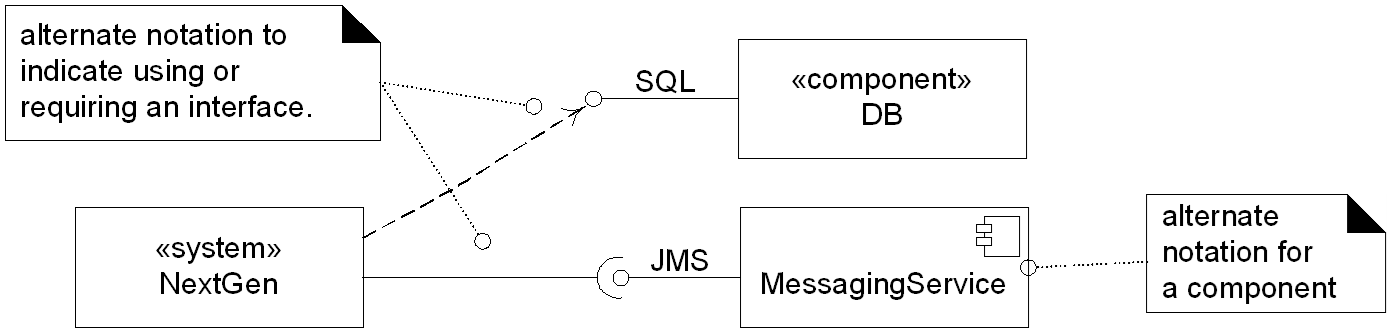
\includegraphics[scale=0.7]{diagramma_componenti/comp_diag_1.png}
\end{center}
\myparagraph{
    L'immagine sopra mostra come può essere dichiarato un componente in un diagramma UML, ovvero tramite notazione <<component>>
    oppure inserendo un simbolo sul lato destro.
    Altra cosa da ricordare è il collegamento tra il sistema e il componente, in base al tipo di freccia, indica se il componente
    sta \textbf{usando} (NextGen usa il DB) o \textbf{richiedendo} (NextGen richiede il MessagingService) \textbf{l'interfaccia}.
}

%DIAGRAMMA DI DISTRIBUZIONE
\mysubsectionformatted{Diagramma di distribuzione}
\myparagraph{
    I diagrammi di distribuzione (o deployment) mostrano l'assegnazione degli artefatti software concreti (es. file eseguibili)
    ai nodi computazionali (es. servizi di elaborazione).
    \\
    Mostrano la distribuzione degli elementi software all'interno dell'architettura fisica e la comunicazione tra questi.
    \\
    L'obiettivo di questo diagramma è quello di comunicare l'architettura fisica o di distribuzione.
}

\subsubsection{Elementi principali del diagramma di distribuzione}

\resizebox{\textwidth}{!}{
    \begin{tabular}{|l|l|}
        \hline
        \textbf{Nodo dispositivo}                 &
        \begin{tabular}[c]{@{}l@{}}Risorsa fisica con servizi di memoria e\\  processazione per eseguire il software.\end{tabular}                                                                                  \\ \hline
        \textbf{Nodo dell'ambiente di esecuzione} &
        \begin{tabular}[c]{@{}l@{}}Risorsa software che viene eseguita all'interno \\ di un nodo esterno (es. computer) e fornisce un servizio\\ per ospitare e eseguire un altro software eseguibile.\end{tabular} \\ \hline
        \textbf{Percorsi di comunicazione}        &
        Connessione tra i nodi.                                                                                                                                                                                     \\
        \hline
    \end{tabular}}

\myparagraph{
    Esempi di diagrammi di distribuzione posso essere degli artefatti, ovvero elementi fisici, come ad esempio \textbf{file eseguibili}
    (file JAR, .exe, script\dots) oppure \textbf{data files} (HTML, XML\dots).
    \\
    Un artefatto "\textbf{manifesta}" uno o più elementi di un modello. Con il termine manifestare si intende che l'artefatto rappresenta
    l'oggetto fisico di uno o più elementi del modello. Questi elementi solitamente sono dei componenti.
}

\newpage
\subsubsection{Esempio di uso di <<manifest>>}
Per rappresentare una manifestazione si usa una linea tratteggiata con freccia aperta etichettata con la keyword <<manifest>>

\begin{center}
    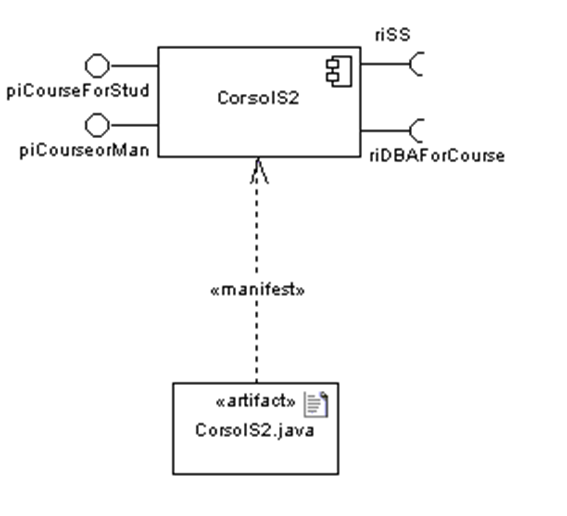
\includegraphics[scale=0.8]{img/diagramma_distribuzione/manifest_dg.png}
\end{center}

\mysubsectionformatted{CBSE, SOSE e Microservizi}
\myparagraph{
    In linea generale sono tre approcci all'ingegneria del software, ciascuno con diverse caratteristiche.
}

\mysubsectionformatted{CBSE - Component Based Software Engineering}
\myparagraph{
    Le parole chiave che determinano questo approccio sono la riusabilità e l'uso di componenti software.
    \\
    Questo approccio nasce dal momento che molto spesso lo sviluppo orientato agli oggetti fallisca per mancanza di riuso
    dei componenti, ciò è causato da vari motivi:

    \begin{enumerate}
        \item Le classi sono troppo dettagliate e specifiche per poter essere riutilizzate in altri contesti.
        \item I componenti sono più astratti delle classi stesse.
        \item I componenti vengono visti come dei provider di servizi indipendenti (stand alone).
        \item I componenti possono esistere come delle entità indipendenti.
    \end{enumerate}

    \newpage

    \noindent L'approccio CBSE fa sì che i componenti forniscano una funzionalità senza dover considerare dove il componente viene
    eseguito o il suo linguaggio di programmazione, questo perché è un'entità eseguibile e indipendente che può essere usato per
    uno o più oggetti eseguibili. L'interfaccia del componente è pubblica e tutte le interazioni avvengono tramite questa.
    \\
    Come per i diagrammi, questo approccio dispone di due tipi di interfacce:
    \vspace{-12pt}

    \begin{center}
        \resizebox{\textwidth}{!}{
            \begin{tabular}{|l|l|}
                \hline
                \textbf{Interfacce Fornite}   &
                \begin{tabular}[c]{@{}l@{}}Definiscono i servizi forniti dal componente verso altri componenti.\\ Essenzialmente, è l'API che definisce i metodi che possono essere chiamati dall'utente.\end{tabular}
                \\ \hline
                \textbf{Interfacce Richieste} &
                \begin{tabular}[c]{@{}l@{}}Definiscono i servizi richiesti dal componente per eseguire quanto specificato.\\ Ciò non compromette l'indipendenza o la distribuzione del componente perché l'interfaccia\\ richiesta non definisce come questi servizi vengono forniti.\end{tabular}
                \\ \hline
            \end{tabular}
        }
    \end{center}

    \vspace{8pt}

    \mysubsubsectionformatted{Componenti essenziali del CBSE}
    \begin{enumerate}
        \item Componenti indipendenti specificati dalle loro interfacce.
        \item Standard specifici dei componenti per facilitare la loro integrazione.\\
              Stabiliscono come i componenti comunicano e operano tra loro.
        \item Middleware che fornisce supporto per la portabilità dl componente.
        \item Un processo di sviluppo mirato al riuso.
    \end{enumerate}

    \mysubsubsectionformatted{Principi di progettazione}
    \begin{enumerate}
        \item I componenti sono indipendenti, non inteferiscono tra loro.
        \item L'implementazione dei componenti è nascosta.
        \item La comunicazione avviene tra interfacce ben definite.
        \item Le piattaforme dei componenti sono condivise in modo da ridurre i costi di sviluppo.
    \end{enumerate}

    I componenti sviluppati tramite diversi approcci NON lavorano tra loro.

    \mysubsubsectionformatted{Elementi basici di un modello di componente}
    \begin{center}
        \resizebox{\textwidth}{!}{%
            \begin{tabular}{|l|l|}
                \hline
                \textbf{Interfacce}    & \begin{tabular}[c]{@{}l@{}}Il modello dei componenti specifica come le interfacce devono essere definite\\ e i suoi elementi (operazioni, nomi, parametri...).\end{tabular}                                    \\ \hline
                \textbf{Uso}           & \begin{tabular}[c]{@{}l@{}}Per essere distribuiti e accessi in remoto, ciascun componente deve avere un\\ nome univoco.\end{tabular}                                                                           \\ \hline
                \textbf{Distribuzione} & \begin{tabular}[c]{@{}l@{}}Il modello dei componenti include una specifica di come i componenti \\ devono essere impacchettati per la loro distribuzione come entità\\ indipendenti e eseguibili.\end{tabular} \\ \hline
            \end{tabular}%
        }
    \end{center}

    \newpage
    \mysubsubsectionformatted{Processi del CBSE}
    I processi del CBSE sono, come dice il nome, dei processi software che supportano l'utilizzo di
    tale approccio. Permettono la riusabilità delle attività di processo coinvolte nelle attività
    di sviluppo e un riuso dei componenti.
    \\
    Bisogna fare una distinzione in merito alla modalità di sviluppo e il riuso:
    \vspace{-12pt}
    \begin{center}
        \resizebox{\textwidth}{!}{
            \begin{tabular}{|l|l|}
                \hline
                \textbf{Sviluppo PER il riuso} & \begin{tabular}[c]{@{}l@{}}Si basa sullo sviluppo di componenti che \\ verranno poi utilizzati in altre applicazioni.\end{tabular} \\ \hline
                \textbf{Sviluppo CON riuso}    & \begin{tabular}[c]{@{}l@{}}Si basa sullo sviluppo di nuove applicazioni\\ usando dei componenti già esistenti.\end{tabular}        \\ \hline
            \end{tabular}%
        }
    \end{center}
    \vspace{8pt}

    \mysubsubsectionformatted{Processi di supporto del CBSE}
    \begin{center}
        \resizebox{\textwidth}{!}{%
            \begin{tabular}{|l|l|}
                \hline
                \textbf{Acquisizione del componente}   & \begin{tabular}[c]{@{}l@{}}Processo che acquisisce i componenti per il loro riuso o trasforma\\ lo sviluppo in un componente riutilizzabile.\end{tabular}                        \\ \hline
                \textbf{Gestione del componente}       & \begin{tabular}[c]{@{}l@{}}Verte sulla gestione dei componenti riusabili assicurandosi\\ siano propriamente catalogati, immagazzinati e resi disponibili per il riuso.\end{tabular} \\ \hline
                \textbf{Certificazione del componente} & Processo che controlla se un componente soddisfa le sue specifiche.                                                                                                                 \\ \hline
            \end{tabular}%
        }
    \end{center}
    \vspace{8pt}

    \mysubsubsectionformatted{CBSE per il riuso}
    Si concentra sullo sviluppo dei componenti. Lo scopo è quello di generalizzare quei componenti che vengono creati per 
    specifiche applicazioni con lo scopo di renderli riutilizzabili.
    \\
    Un componente ha più probabilità di essere riutilizzato se è associato a un'astrazione di dominio stabile, ovvero a un oggetto
    di business ben definito e costante nel sistema.
    \\
    Per fare un esempio di dominio stabile può essere un ospedale, dove i componenti hanno ciascuno degli scopi fontamentali 
    (dottori, pazienti, trattamenti ecc\dots)

    \newpage
    \mysubsubsectionformatted{CBSE con riuso}
    Al contrario della prima tipologia, questa cerca e integra componenti già esistenti.
    Quando si riutilizzano i componenti in un progetto software, è fondamentale considerare i compromessi tra i requisiti ideali 
    di ciò che si desidererebbe avere e i servizi reali forniti dai componenti disponibili.
    \\
    Questo approccio richiede:
    \begin{enumerate}
        \item Sviluppo dei requisiti preliminari (essenziali).
        \item Ricerca dei componenti e la loro modifica in base alle funzionalità disponibili.
        \item Cercare nuovamente per trovare componenti migliori che soddifsano i requisiti.
        \item Unire (o comporre) i componenti per creare il sistema.
    \end{enumerate}

    \mysubsubsectionformatted{Problemi ancora aperti con CBSE}
    \begin{enumerate}
        \item Quanto è affidabile un componente senza un codice sorgente disponibile?
        \item Chi certifica la qualità dei componenti?
        \item Come possono essere predette le proprietà emergenti della composizione dei componenti?
        \item Come si fanno le analisi tra le caratteristiche di un componente con un altro?
    \end{enumerate}
}
    \newpage

\mysubsectionformatted{SOSE - Service Oriented Software Engineering}
\myparagraph{
    Le parole chiave che determinano questo approccio sono la riusabilità e l'uso di servizi software (per il CBSE era l'uso
    dei componenti software).
    \\
    Questo approccio nasce con lo scopo di fornire lo stesso servizio a più applicazioni o utenti, questo perché i servizi
    sono indipendenti tra loro.
    \\
    Per servizio si intende un'entità software con basso accoppiamento (loosely-coupled) che incapsula delle funzionalità che
    possono essere distribuite e accesse.

    \mysubsubsectionformatted{Standard di SOSE}
    \begin{center}
        \begin{tabularx}{\textwidth}{|>{\centering}m{2cm}|X|}
            \hline
            \textbf{SOAP} & Protocollo di accesso agli oggetti che definisce un'organizzazione per lo scambio di dati strutturati tra i web services.                                          \\ \hline
            \textbf{WSDL} & Definisce come possono essere rappresentate le interfacce dei web services.                                                                                        \\ \hline
            \textbf{UDDI} & Standard di ricerca che definisce come possono essere organizzate le informazioni di descrizione dei servizi, utilizzate dai richiedenti dei servizi per trovarli. \\ \hline
        \end{tabularx}
    \end{center}

    \subsubsection{Illustrazione dell'approccio SOSE}
    \begin{center}
        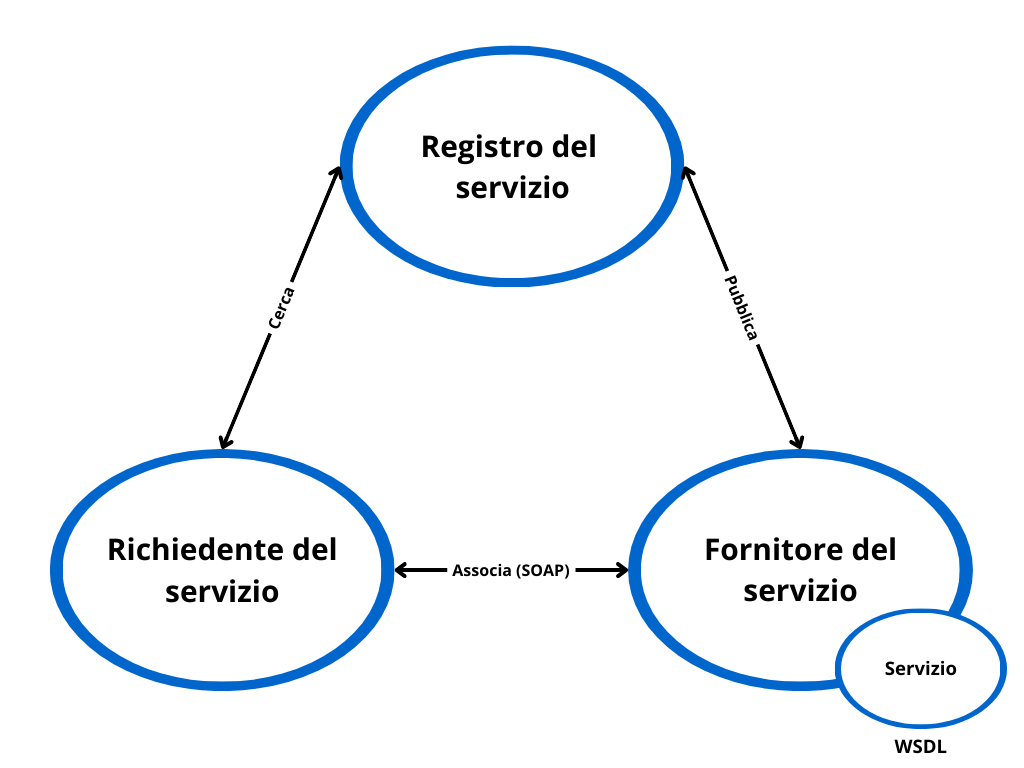
\includegraphics[width=10cm]{sose/funzionamento_sose.png}
    \end{center}
    \newpage

    \noindent Come per CBSE, anche SOSE distingue, nel suo caso, i servizi PER il riuso e i servizi CON riuso:
    \mysubsubsectionformatted{Servizi per il riuso}
    Come dice il titolo, questi servizi vengono sviluppati con lo scopo di essere riutilizzati all'interno di applicazioni orientati
    ai servizi. Questi servizi devono essere progettati come delle 'astrazioni riutilizzabili' che possono essere usati in sistemi diversi,
    in modo da poter garantire un servizio robusto e affidabile. Alla fine, il servizio deve essere ben documentato
    in modo da poter essere scoperto e capito da potenziali utenti.

    \mysubsubsectionformatted{Servizi con riuso}
    I servizi in questo caso vengono visti come dei componenti riutilizzabili. In questo modo, i servizi possono essere forniti localmente o
    esternamente verso altri fornitori. Altro vantaggio è che i servizi sono indipendenti dal linguaggio in cui vengono scritti, e per concludere
    l'investimento fatto in sistemi informatici obsoleti può essere preservato, conservandone quindi il valore attraverso aggiornamenti o
    modernizzazioni.

    \mysubsubsectionformatted{CBSE vs SOSE}
    La differenza sostanziale tra i due è che CBSE fa uso dei componenti, SOSE dei servizi.
    \begin{enumerate}
        \item I servizi sono indipendenti, i componenti no.
        \item I servizi non possiedono alcuna interfaccia 'richiesta'.
        \item La comunicazione tra i servizi avviene tramite messaggi in formato XML.
    \end{enumerate}
    \newpage
}

\mysubsectionformatted{MS - Microservices Software Engineering}
\myparagraph{
    Si tratta di uno stile architetturare che struttura l'applicazione come una\\ collezione
    di piccoli e contenuti componenti con basso accoppiamento. Questi componenti vengono anche
    chiamati servizi e implementano delle specifiche capacità di business.
    \\
    Tra le caratteristiche dei microservizi troviamo:
    \begin{enumerate}
        \item Comunicazione attraverso protocolli leggeri (lightweight).
        \item Sviluppati da team dedicati.
        \item La distribuzione è indipendente.
    \end{enumerate}
    L'obiettivo principale dei microservizi sarebbe quello di garantire scalabilità,\\ affidabilità, eterogeneità
    tecnologica e aggiornamenti continui del codice,\\ purtroppo, nella realtà ci troviamo di fronte a una
    complessa manutenibilità e una fase di testing difficile.

    \begin{center}
        \resizebox{\columnwidth}{!}{
            \begin{tabular}{c|c|c|}
                \cline{2-3}
                \multicolumn{1}{l|}{}                                                                                & \cellcolor[HTML]{3531FF}{\color[HTML]{FFFFFF} SOSE}                                                                                               & \cellcolor[HTML]{3531FF}{\color[HTML]{FFFFFF} MS}                                                                         \\ \hline
                \multicolumn{1}{|c|}{\textbf{Obiettivo}}                                                             & Riusabilità dei servizi                                                                                                                           & Garantire basso accoppiamento                                                                                             \\ \hline
                \multicolumn{1}{|c|}{\textbf{\begin{tabular}[c]{@{}c@{}}Di cosa\\ fa uso\end{tabular}}}              & \begin{tabular}[c]{@{}c@{}}Servizi: include tante funzionalità\\ di business e spesso è implementato\\ come un completo sottosistema\end{tabular} & \begin{tabular}[c]{@{}c@{}}Micro-servizi: creati per servire\\ solo una specifica funzionalità\\ di business\end{tabular} \\ \hline
                \multicolumn{1}{|c|}{\textbf{\begin{tabular}[c]{@{}c@{}}Cosa succede \\ alla modifica\end{tabular}}} & \begin{tabular}[c]{@{}c@{}}Richiede la modifica del sistema\\ monolitico, una modifica significativa\end{tabular}                                 & \begin{tabular}[c]{@{}c@{}}Richiede la creazione di un \\ nuovo servizio\end{tabular}                                     \\ \hline
                \multicolumn{1}{|c|}{\textbf{Comunicazione}}                                                         & Tramite ESB (Enterprise Service Bus)                                                                                                              & \begin{tabular}[c]{@{}c@{}}Meno elaborata e semplice \\ sistema di messaggi\end{tabular}                                  \\ \hline
                \multicolumn{1}{|c|}{\textbf{Protocolli}}                                                            & Multipli protocolli per messaggi (SOAP)                                                                                                           & Protocolli leggeri (HTTP, REST)                                                                                           \\ \hline
                \multicolumn{1}{|c|}{\textbf{Distribuzione}}                                                         & \begin{tabular}[c]{@{}c@{}}Uso di una piattaforma comune per\\ la distribuzione di tutti i servizi\end{tabular}                                   & \begin{tabular}[c]{@{}c@{}}Uso di una piattaforma cloud\\ per la distribuzione\end{tabular}                               \\ \hline
                \multicolumn{1}{|c|}{\textbf{Container}}                                                             & Uso poco popolare (Docker o Kubernates)                                                                                                           & Uso molto popolare                                                                                                        \\ \hline
                \multicolumn{1}{|c|}{\textbf{\begin{tabular}[c]{@{}c@{}}Archiviazione\\ dei dati\end{tabular}}}      & Condivisi tra i diversi servizi                                                                                                                   & \begin{tabular}[c]{@{}c@{}}Ogni micro-servizio può avere\\ un proprio archivio indipendente\end{tabular}                  \\ \hline
            \end{tabular}%
        }
    \end{center}
    \newpage
}

\mysubsectionformatted{Cloud Computing}
\myparagraph{
    Nasce per mano del NIST (National Instituite of Standard and Technology), si tratta
    di un modello capace di garantire un accesso via rete a una vasta area di risorse
    (reti, server, applicazioni, servizi ecc...) che possono essere rilasciate con la
    minima gestione o interazione con il fornitore del servizio.
    \\
    Tra le caratteristiche principali abbiamo:
    \begin{enumerate}
        \item Capacità per un utente di registrarsi e ricevere i servizi senza dover affrontare
              lunghe attese.
        \item Capacità di accedere ai servizi mediante piattaforme standard (desktop, laptop ecc\dots)
        \item Le risorse sono messe in comune tra tutti gli utenti o clienti.
        \item Scalabilità rapida per far fronte a un grande quantitativo di utenti.
        \item La fatturazione del servizio è monitorato in base a quanto si sta usando quel servizio.
    \end{enumerate}

    \mysubsubsectionformatted{La gerarchia del Cloud}
    \vspace{-1cm}
    \begin{center}
        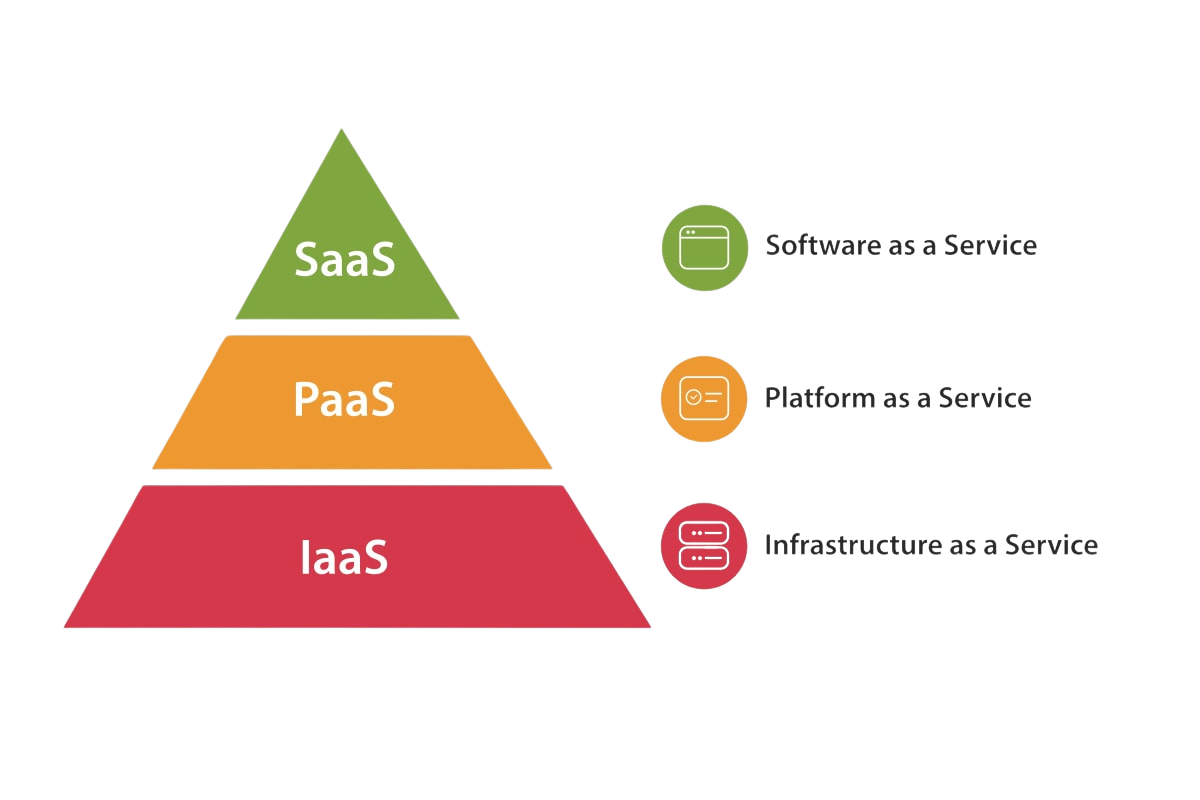
\includegraphics[width=13cm]{cloud/gerarchia_cloud.jpg}
    \end{center}

    \begin{center}
        \resizebox{\columnwidth}{!}{%
            \begin{tabular}{|l|l|}
                \hline
                \cellcolor[HTML]{009901}{\color[HTML]{FFFFFF} \textbf{SaaS}} & Applicazioni rivolte agli utenti finali, inviati tramite il web                                                                                  \\ \hline
                \cellcolor[HTML]{F56B00}{\color[HTML]{FFFFFF} \textbf{PaaS}} & \begin{tabular}[c]{@{}l@{}}Set di strumenti e servizi per creare codici e distribuire\\ le applicazioni in modo rapido e efficiente\end{tabular} \\ \hline
                \cellcolor[HTML]{CB0000}{\color[HTML]{FFFFFF} \textbf{IaaS}} & \begin{tabular}[c]{@{}l@{}}Hardware e software che da vita a tutti i servizi (server, \\ reti, sistemi operativi ecc\dots)\end{tabular}          \\ \hline
            \end{tabular}%
        }
    \end{center}
}

\mysectionformatted{Progettazione dell'architettura Software e Design Principle}
\myparagraph{
    Il capitolo ha lo scopo di introdurre i design pattern per progettare l'architettura
    logica del sistema
}

\mysubsectionformatted{Analisi Architetturale}
\myparagraph{
    L'analisi architetturale ha l'obiettivo di indentificare e risolvere i requisiti non
    funzionali del sistema (es. la sicurezza) nel contesto dei requisiti funzionali.
    \\
    Ricordiamo il documento che definisce i requisiti non funzionali, ovvero
    le \\ \coloredtext[blue]{specifiche supplementari}.
    \\
    I passi da seguire durante l'analisi sono:
    \begin{enumerate}
        \item \textbf{Investigazione}: identificazione di requisiti funzionali e non funzionali
              che hanno maggiore impatto sul sistema.
        \item \textbf{Progettazione}: risoluzione dei requisiti identificati.
    \end{enumerate}
    Per i requisiti che hanno impatto architetturale significativo si analizzano le
    alternative e si creano delle soluzioni per gestire i compromessi e le priorità.

    \mysubsubsectionformatted{Collezione e organizzazione dei requisiti non funzionali}
    Viene stilata la seguente tabella per i requisiti non funzionali:
    \vspace{-0.1cm}

    \begin{center}
        \renewcommand{\arraystretch}{1.5}
        \resizebox{\columnwidth}{!}{%
            \begin{tabular}{|ll|}
                \hline
                \multicolumn{2}{|c|}{\cellcolor[HTML]{3531FF}{\color[HTML]{FFFFFF} \textbf{Tabella dei fattori}}}                                                                                               \\ \hline
                \multicolumn{1}{|l|}{\textbf{Nome fattore}}                & Nome del fattore (requisito)                                                                                                                \\ \hline
                \multicolumn{1}{|l|}{\textbf{Misure e scenari di qualità}} & Come il fattore sarà misurato e valutato tramite metriche di qualità                                                                        \\ \hline
                \multicolumn{1}{|l|}{\textbf{Variabilità}}                 & \begin{tabular}[c]{@{}l@{}}Quanto il sistema è flessibile a soddisfare il requisito \\ con possibilità di evoluzione in futuro\end{tabular} \\ \hline
                \multicolumn{1}{|l|}{\textbf{Impatto del fattore}}         & Quanto influisce il fattore sull'architettura del sistema                                                                                   \\ \hline
                \multicolumn{1}{|l|}{\textbf{Priorità per il successo}}    & Quanto è importante il fattore per il successo del sistema                                                                                  \\ \hline
                \multicolumn{1}{|l|}{\textbf{Difficoltà o rischi}}         & Possibili difficoltà associate al soddisfacimento di questo requisito                                                                       \\ \hline
            \end{tabular}%
        }
    \end{center}
    

    \mysubsubsectionformatted{Gerarchia di obiettivi per le decisioni architetturali}
    Esistono 3 tipi di obiettivi e priorità:
    \begin{enumerate}
        \item Vincoli inflessibili: sicurezza, conformità alle leggi\dots
        \item Obiettivi di business: tipi di clienti finali interessati al prodotto software
        \item Altri obiettivi: estensioni con altre funzionalità
    \end{enumerate}

    \mysubsubsectionformatted{Principi di base della progettazione architetturale}
    Sono dei principi che offrono maggiore efficienza all'architettura software:
    \begin{center}
        \resizebox{0.4\columnwidth}{!}{%
            \begin{tabular}{|c|}
                \hline
                \rowcolor[HTML]{3166FF}
                \multicolumn{1}{|c|}{\cellcolor[HTML]{3166FF}{\color[HTML]{FFFFFF} \textbf{Principi}}}               \\ \hline
                Accoppiamento basso                                                                                  \\ \hline
                Coesione alta                                                                                        \\ \hline
                Variazione protetta                                                                                  \\ \hline
                \begin{tabular}[c]{@{}l@{}}Separazione degli interessi e \\ localizzazione dell'impatto\end{tabular} \\ \hline
                \begin{tabular}[c]{@{}l@{}}Utilizzo di pattern e \\ stili architetturali\end{tabular}                \\ \hline
            \end{tabular}%
        }
    \end{center}

    \mysubsubsectionformatted{L'architettura logica}
    Questo tipo di architettura vede il sistema come un insieme di package logici. Descrive il sistema nei termini della
    sua organizzazione in layers, packages, frameworks, classi, interfacce e sottosistemi.
    \\
    I\textbf{ \coloredtext[blue]{package}} raggruppano un insieme di responsabilità coese
    (strettamente correlate tra loro), questa caratteristica viene definita anche come
    \textbf{ \coloredtext[blue]{modularizzazione}}.
    \\
    Questa caratteristica favorisce una separazione degli interessi (separation of concerns).
    \\
    Ciascun package si occupa di quello per cui è stato progettato, senza preoccuparsi del resto del sistema.

    \mysubsubsectionformatted{I pattern}
    I pattern si dividono in diverse tipologie:
    \vspace{-0.5cm}
    \begin{center}
        \resizebox{\columnwidth}{!}{%
            \begin{tabular}{|
                    >{\columncolor[HTML]{3166FF}}l |l|}
                \hline
                {\color[HTML]{FFFFFF} \textbf{Pattern architetturali}} & Progettazione a larga scala (es. i pattern layers)                                                                                                                                    \\ \hline
                {\color[HTML]{FFFFFF} \textbf{Design patterns}}        & \begin{tabular}[c]{@{}l@{}}Progettazione a scala media-piccola che hanno\\ connessioni fra gli elementi a larga scala (es. i pattern GoF)\end{tabular}                                \\ \hline
                {\color[HTML]{FFFFFF} \textbf{Idiomi}}                 & \begin{tabular}[c]{@{}l@{}}Soluzioni progettuali di basso livello legate al linguaggio\\ o alle implementazioni usate (es. comparazione di due stringhe,\\ Singleton...)\end{tabular} \\ \hline
                {\color[HTML]{FFFFFF} \textbf{Strategie}}              & \begin{tabular}[c]{@{}l@{}}Direttive e consigli pratici su come risolvere un certo problema\\ in modo efficace.\end{tabular}                                                          \\ \hline
            \end{tabular}%
        }
    \end{center}
    Per chiarire meglio la differenza tra i pattern architetturali e i design pattern ci si può riferire alle
    seguenti domande:
    \begin{itemize}
        \item Quali sono le parti fondamentali del sistema? \rightarrow \vspace{0.25em} Pattern architetturali
        \item Come sono connesse tra loro? \rightarrow \vspace{0.25em} Design patterns
    \end{itemize}

    \mysubsubsectionformatted{Problemi nelle architetture software}
    Si possono verificare diverse problematiche durante lo sviluppo dell'architettura software:
    \begin{enumerate}
        \item Alto accoppiamento dei componenti, portano alla modifica di più elementi in caso di cambiamento.
        \item La logica applicativa condivisa con le GUI.
        \item I servizi tecnici direttamente collegati alla logica applicativa, sfavorendone il riuso.
        \item L'evoluzione del sistema risulta difficoltosa dato l'alto accoppiamento e le numerose funzionalità
              distinte e non correlate tra loro.
        \item Ovviamente possono esserci tante altre problematiche\dots
    \end{enumerate}
}

\mysubsubsectionformatted{Il Pattern architetturale "Layers"}
\myparagraph{
    Questo pattern permette di risolvere i problemi elencati in precedenza tramite l'uso dei layers.
    \\
    Un \textbf{\coloredtext[blue]{Layer}} è un elemento di grandi dimensioni, spesso composto da molti\\ package e sottosistemi.
    \begin{tcolorbox}[colback=blue!5!white, colframe=blue!75!black]
        Il pattern permette di organizzare l'architettura logica in un sistema a più livelli (layers) che
        comprendono funzionalità distinte ma correlate in modo da permettere una netta separazione delle responsabilità
        e un aumento della coesione del sistema stesso.
        \\
        I livelli più bassi comprendono i servizi più generali e di basso livello, quelli in alto saranno più specifici
        per la singola applicazione.
    \end{tcolorbox}
    \noindent Il numero di layer e il loro scopo non è fisso, cambia a seconda delle applicazioni. Ciascun layer si appoggia alle
    funzionalità dei layer sottostanti, ma possono comunicare anche con i layer di livelli più bassi. Ovviamente, come il sistema stesso,
    anche l'architettura a layer viene sviluppata in modo iterativo, l'obiettivo è quello di avere
    l'architettura fondamentale stabilita.
    \newpage
    \subsubsection{Esempio di architettura a layers}
    \begin{center}
        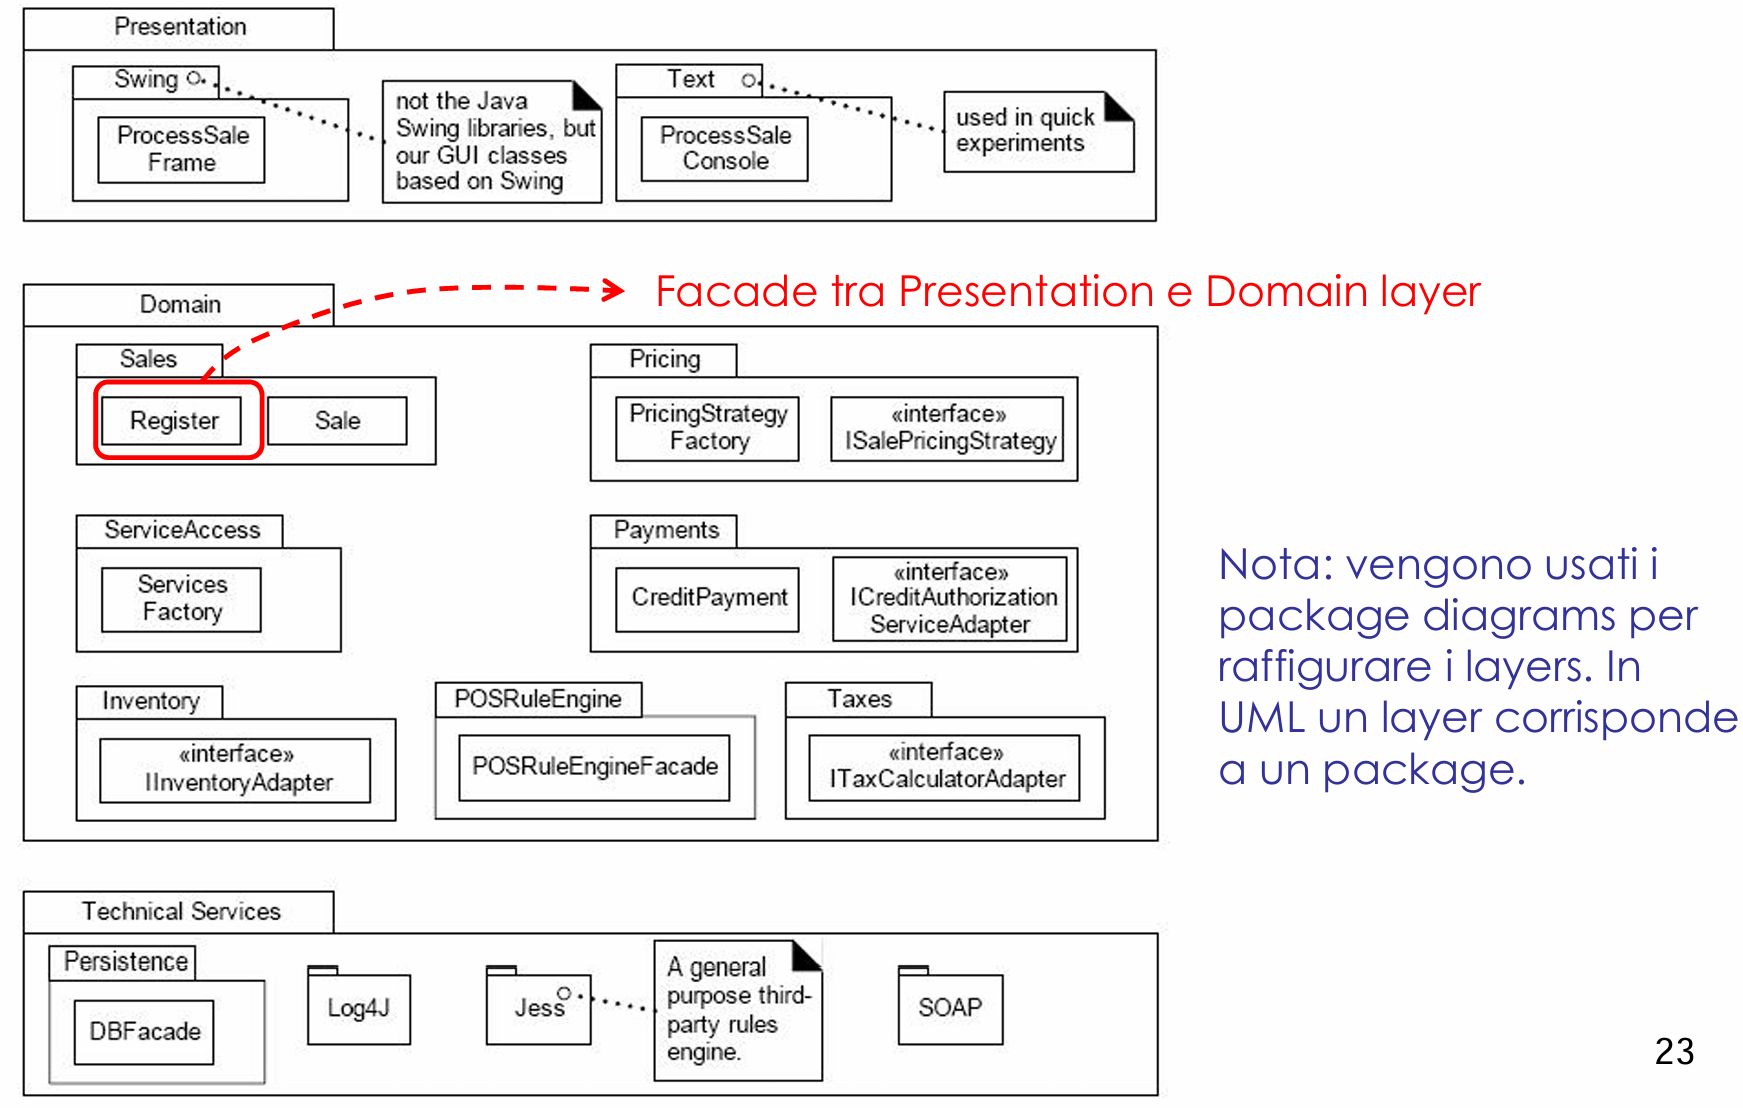
\includegraphics[scale=0.27]{architettura_layer/archi_layer_esempio.png}
    \end{center}
    \mysubsubsectionformatted{Considerazioni sull'Application Layer}
    \begin{itemize}
        \item Per conoscere lo stato del client si fa uso dei package Presentation e Domain. I due package collaborano tra loro
              per controllare il flusso di lavoro (l'ordine delle finestre, le pagine web\dots)
        \item L'Application Layer viene usato quando:
              \begin{enumerate}
                  \item Sono disponibili più interfacce utente. In questo caso vengono usati degli Adapter per collezionare i dati delle varie
                        interfacce e le Facade per nascondere l'accesso al Domain.
                  \item Il sistema è distribuito e il Domain si trova su un nodo diverso rispetto al Presentation.
                  \item Il Domain non può mantenere lo stato delle sessioni.
                  \item Esiste un workflow ben definito da seguire nella presentazione delle varie schermate.
              \end{enumerate}
    \end{itemize}
    \newpage
    \noindent Ovviamente esisteranno accoppiamenti fra i vari livelli, ma si possono raffigurare i più significativi
    attraverso un apposito diagramma.
    \begin{center}
        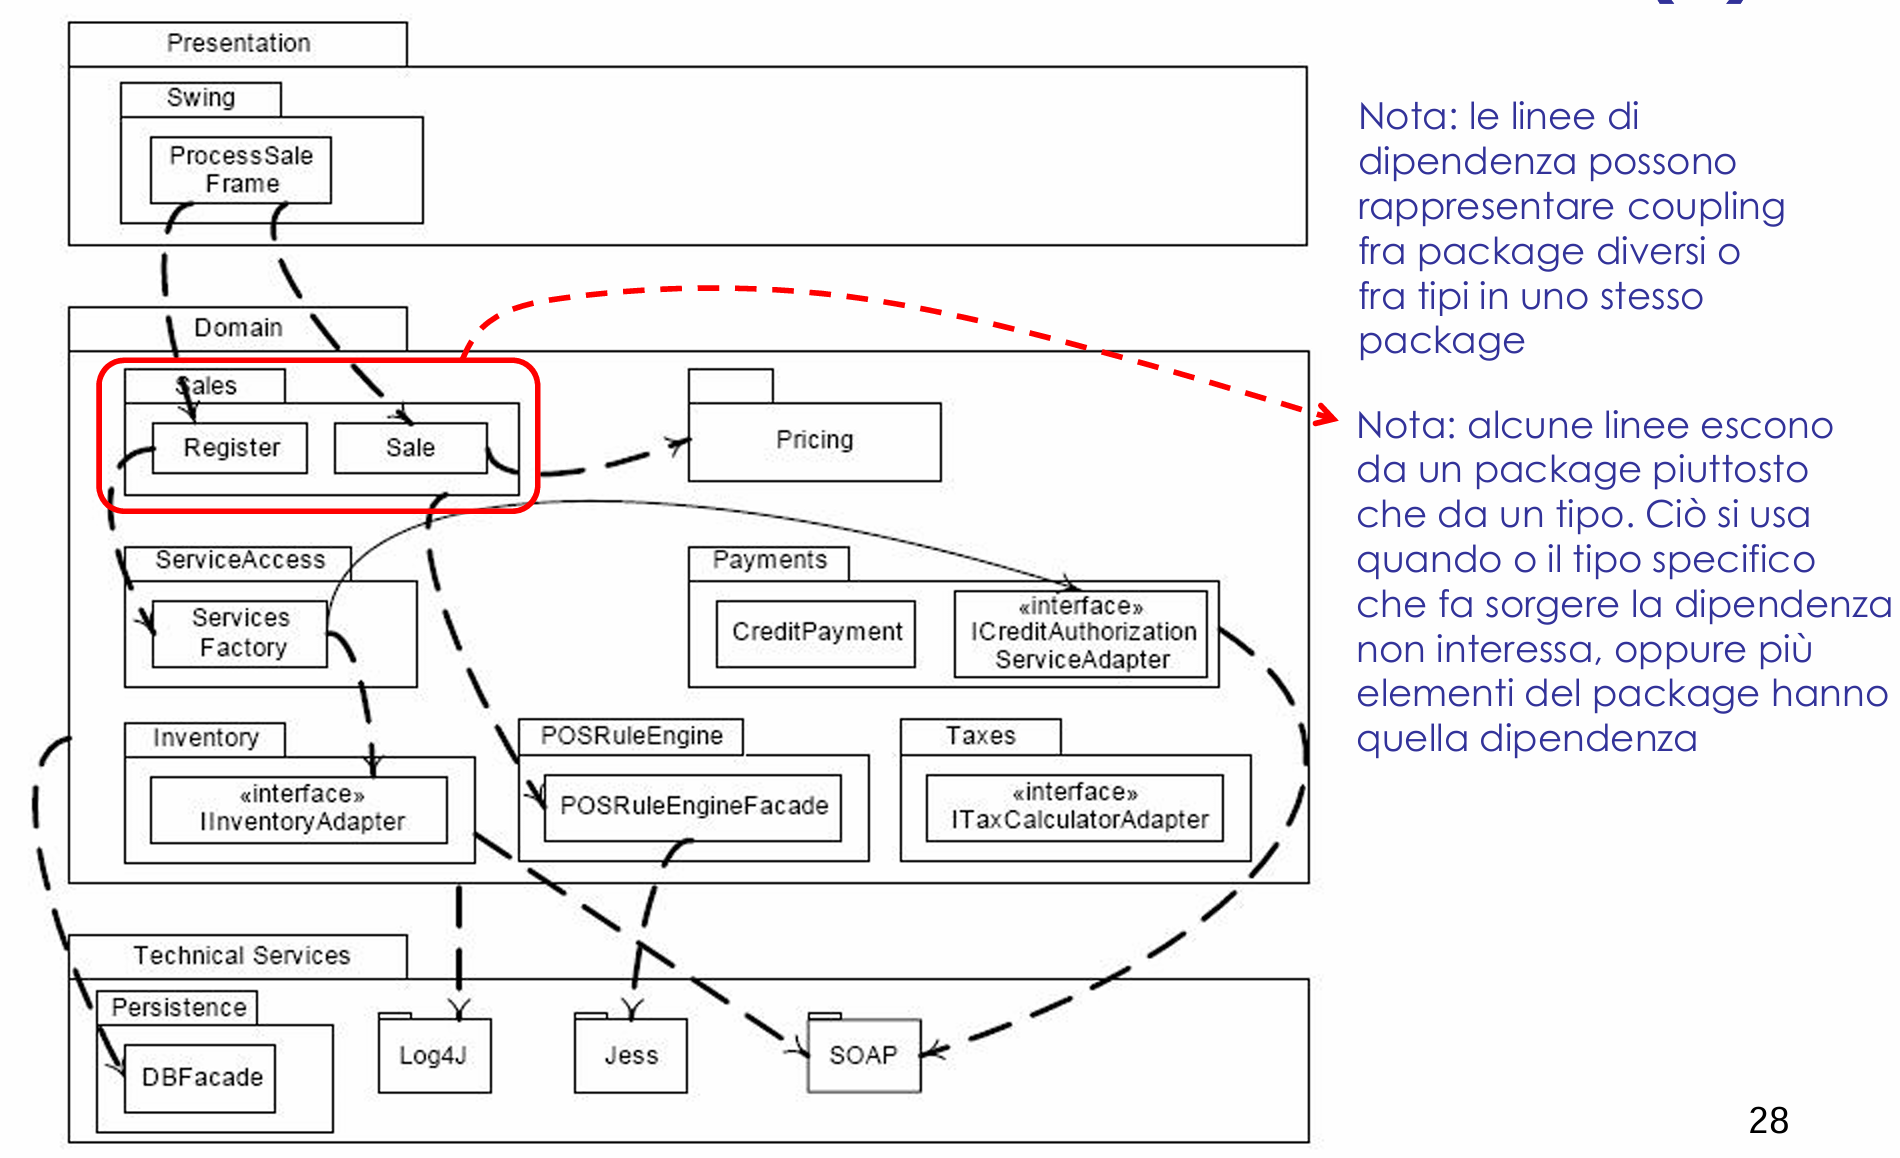
\includegraphics[scale=0.25]{architettura_layer/archi_layer_accoppiamenti.png}
    \end{center}
    Per capire meglio come gli oggetti fra i vari layer comunicano fra di loro si possono usare i \textbf{Diagrammi di Sequenza} in
    modo da rappresentare gli scenari architetturali più significativi.
    \subsubsection{Esempio di diagramma di sequenza}
    \begin{center}
        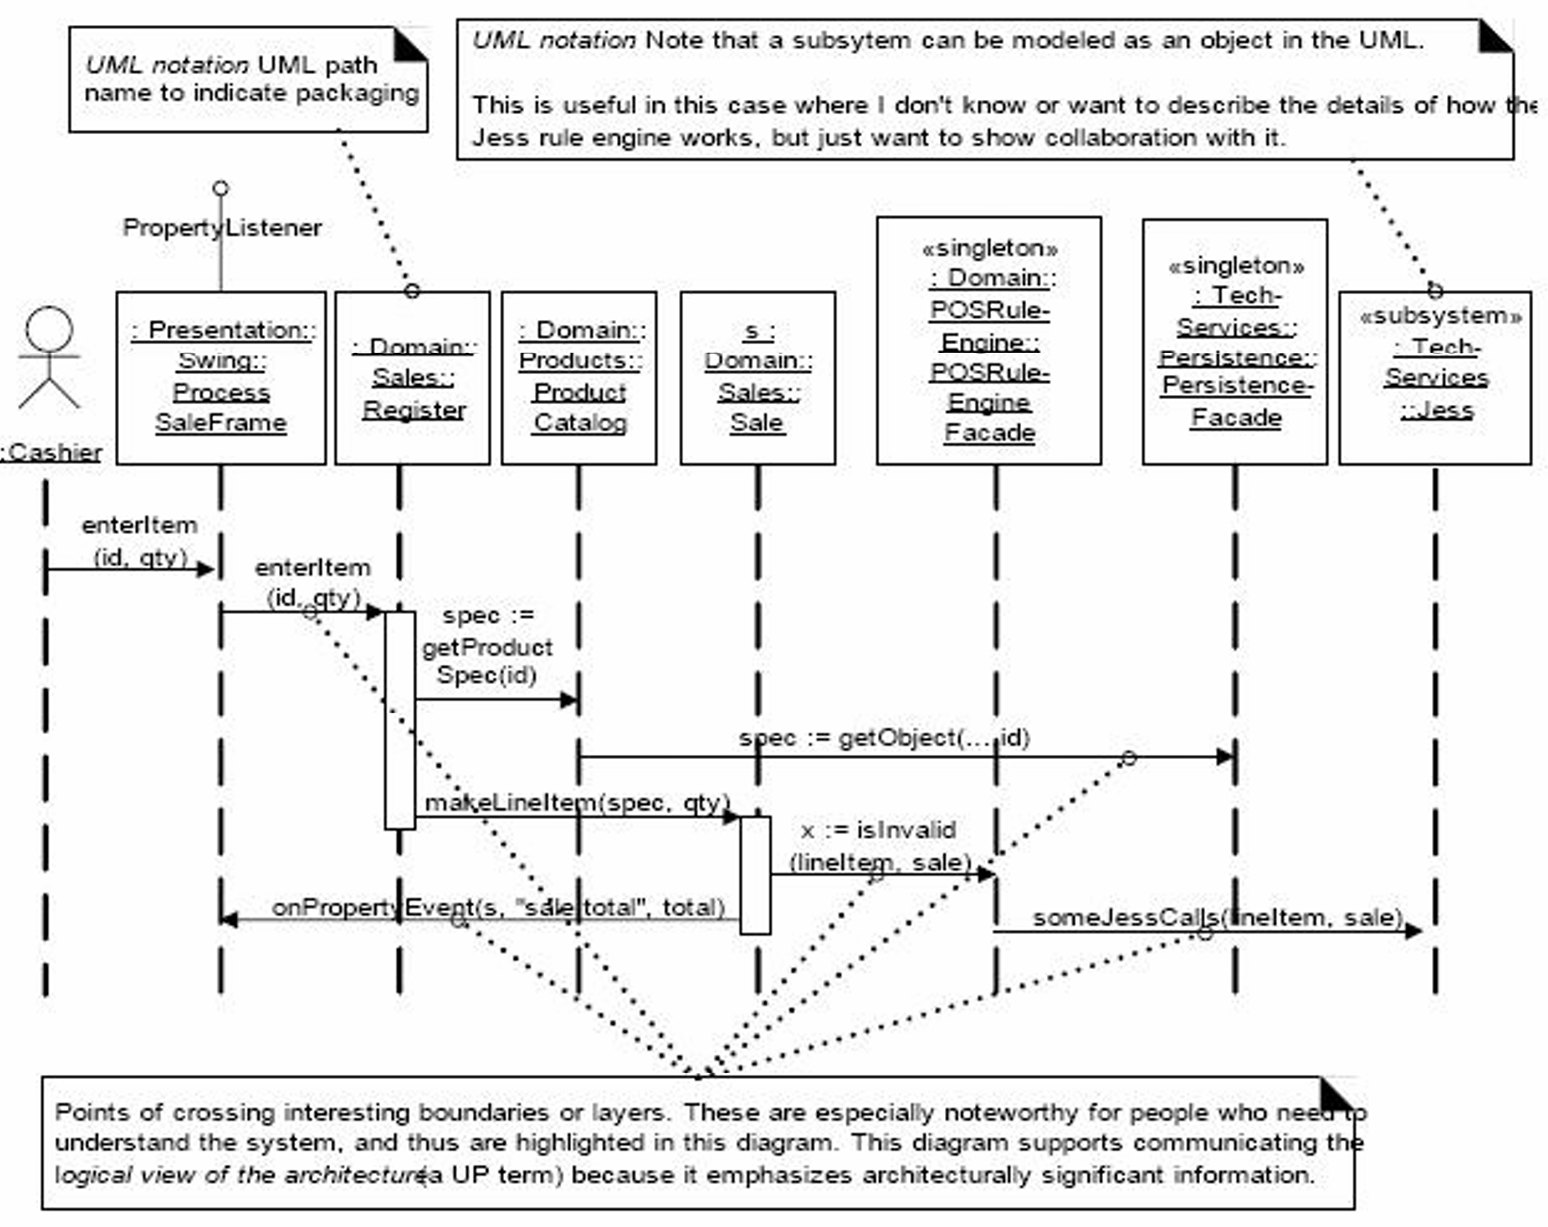
\includegraphics[scale=0.23]{architettura_layer/diagramma_sequenza.png}
    \end{center}
    \newpage
    \noindent Nel diagramma si possono fare delle considerazioni:
    \begin{enumerate}
        \item In UML si può illustrare il nome del package a cui una certa classe appartiene con la seguente dicitura: \textit{<PackageName>::<TypeName>}.
              Ciò permette di evidenziare le connessioni fra package e layer all'interno di un diagramma dinamico.
        \item Lo sterotipo \textit{<<subsystem>>} indica un'entità con il suo comportamento e le sue interfacce. Può essere modellato da un package
              o da un oggetto.
        \item Il diagramma di sequenza mostra solo le relazioni rilevanti dal punto di vista architetturale.
    \end{enumerate}
    Bisogna precisare che alcuni package rappresentano veri e propri sottosistemi indipendenti (stereotipi),
    con il proprio comportamento e le loro interfacce. Altri package \textbf{NON} sono sottosistemi.

    \mysubsubsectionformatted{Collaborazione tra pattern Layers e design pattern}
    Come detto prima, il pattern architetturale serve per definire le parti più grandi del sistema. Per poter stabilire le
    connessioni tra gli stati e i package verranno usati i design pattern. Spesso sono usati il \textbf{Facade}, \textbf{Observer},
    e \textbf{Controller}, quindi i pattern GRASP.

    \mysubsubsectionformatted{Funzionamento del Facade}
    Viene utilizzato per accedere alle funzionalità offerte da un sottosistema. Facade permette di nascondere il sottosistema dietro un'interfaccia
    unificata. Facade non espone le operazioni di basso livello, ma quelle di alto livello utilizzabili dai client.
    \begin{center}
        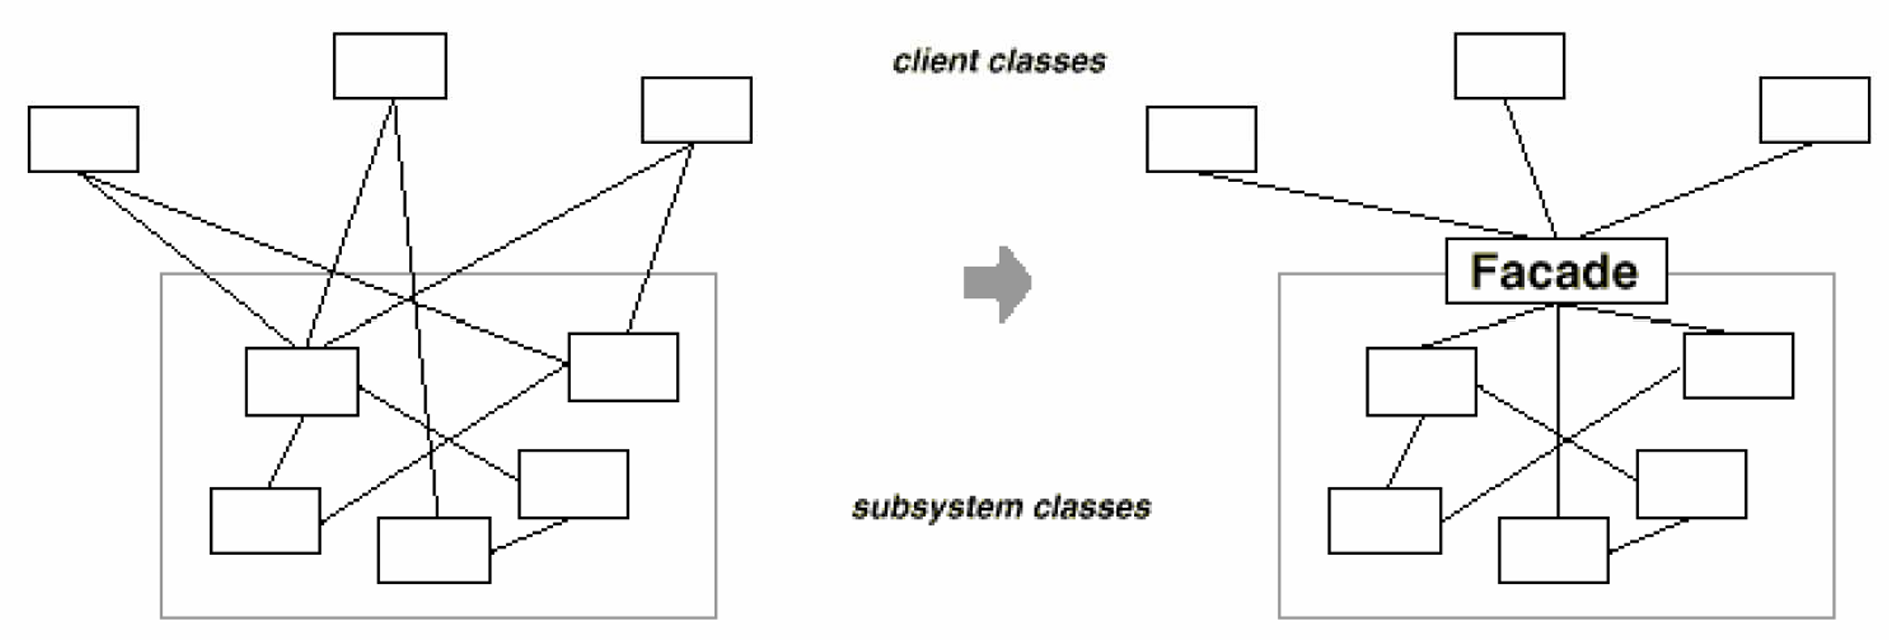
\includegraphics[scale=0.25]{architettura_layer/facade.png}
    \end{center}
    \newpage
    \mysubsubsectionformatted{Funzionamento del Controller}
    Viene utilizzato per descrivere le scelte comuni tipiche degli handler lato client per le richieste di operazioni di sistema provenienti
    dal Presentation Layer (UI).
    \begin{center}
        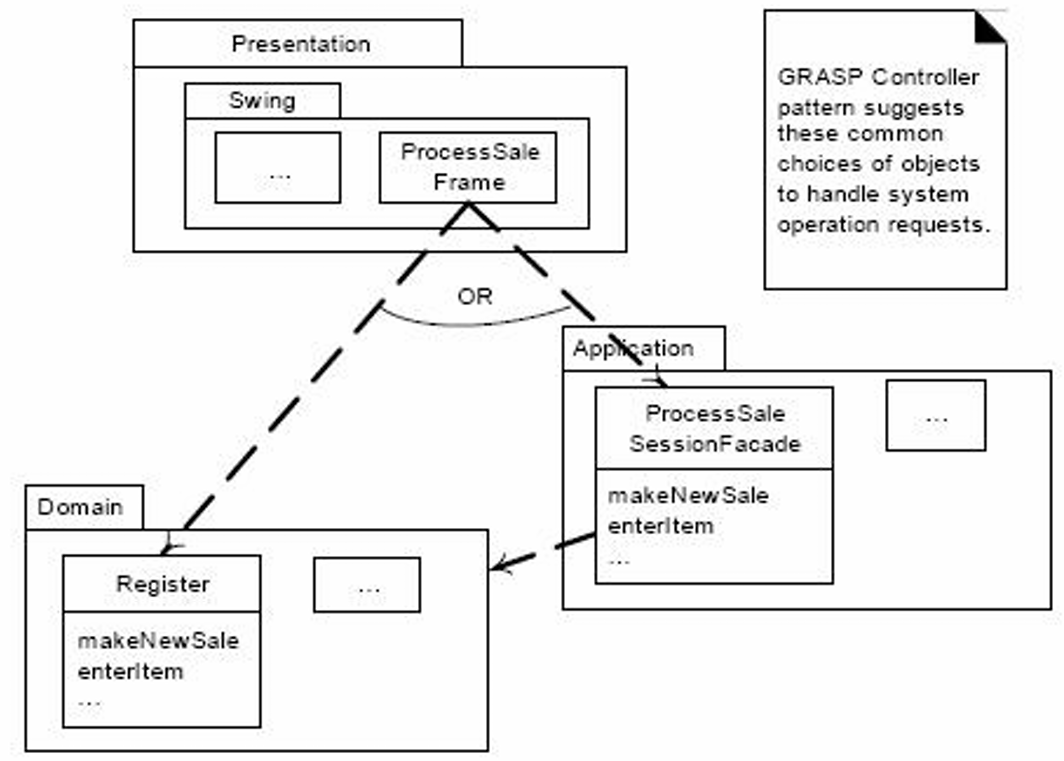
\includegraphics[scale=0.32]{architettura_layer/controller.png}
    \end{center}
    Si tratta quindi del primo oggetto oltre lo stato UI che coordina le operazioni di sistema, in grado di ricevere e gestire un messaggio di un'operazione
    di sistema. Quando si parla di operazioni di sistema si intendono gli eventi di input principali del sistema.
    \\
    Tra i vantaggi del Controller abbiamo:
    \begin{enumerate}
        \item Logica applicativa non gestita nello strato di interfaccia.
        \item Riuso della logica.
        \item Si possono usare interfacce diverse.
    \end{enumerate}
    Quando si usano i Controller, accade di compiere l'errore di "gonfiarlo":
    \begin{itemize}
        \item Un solo Controller riceve numerosi eventi di sistema.
        \item Il Controller svolge parte del lavoro prima di delegarlo.
        \item Il Controller ha numerosi attributi e conserva le informazioni sul sistema e sul dominio.
    \end{itemize}
    \newpage
    
    \noindent Un modo per vedere le operazioni di sistema è tramite i \textbf{Diagrammi di Interazione}.
    \begin{center}
        \includegraphics[scale=0.28]{architettura_layer/diagramma_attività.png}
    \end{center}

    \mysubsubsectionformatted{Funzionamento di Observer}
    Ipotizzando che il layer Application o Domain debbano comunicare con il Presentation, l'Observer è utile al caso.
    \\
    Questo design pattern permette di notificare e aggiornare automaticamente tutti gli oggetti dipendenti da un'oggetto 'padre'
    che prende il nome di Subject.
    \begin{center}
        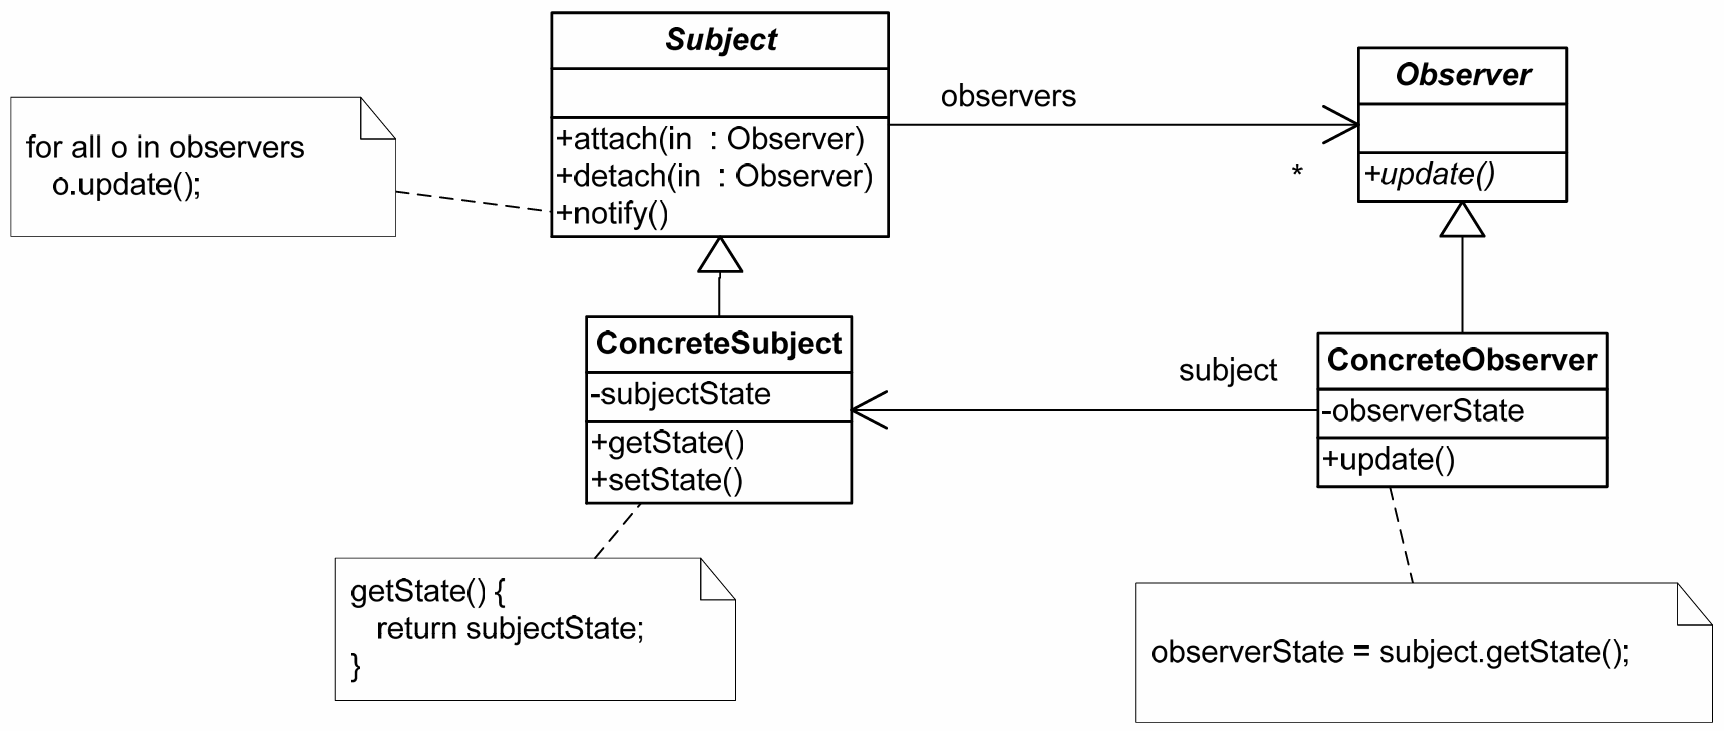
\includegraphics[scale=0.27]{architettura_layer/observer.png}
    \end{center}
    \newpage
}

\mysubsubsectionformatted{Model-View Separation}
\myparagraph{
    Si tratta di un approccio che ha l'obiettivo di separare il layer Domain (Model) dal layer Presentation (View).
    Gli oggetti del Domain non devono avere\\ conoscenza degli oggetti del Presentation.
    \\
    Esistono diverse motivazioni per usare questo approccio:
    \begin{enumerate}
        \item Si ha un modello coeso.
        \item Sviluppo separato del modello e l'interfaccia grafica.
        \item Permette di connettere facilmente nuove viste.
        \item Permette l'esecuzione del modello indipendentemente dalla GUI.
    \end{enumerate}
    Model-View Separation adotta una comunicazione verso l'alto.
}

\mysubsubsectionformatted{Architettura a strati rilassata}
\myparagraph{
    Come accennato in precedenza, i livelli di un'architettura a layer non comunicano solo con il livello
    sottostante. Si parla quindi di struttura rilassata.

    \begin{center}
        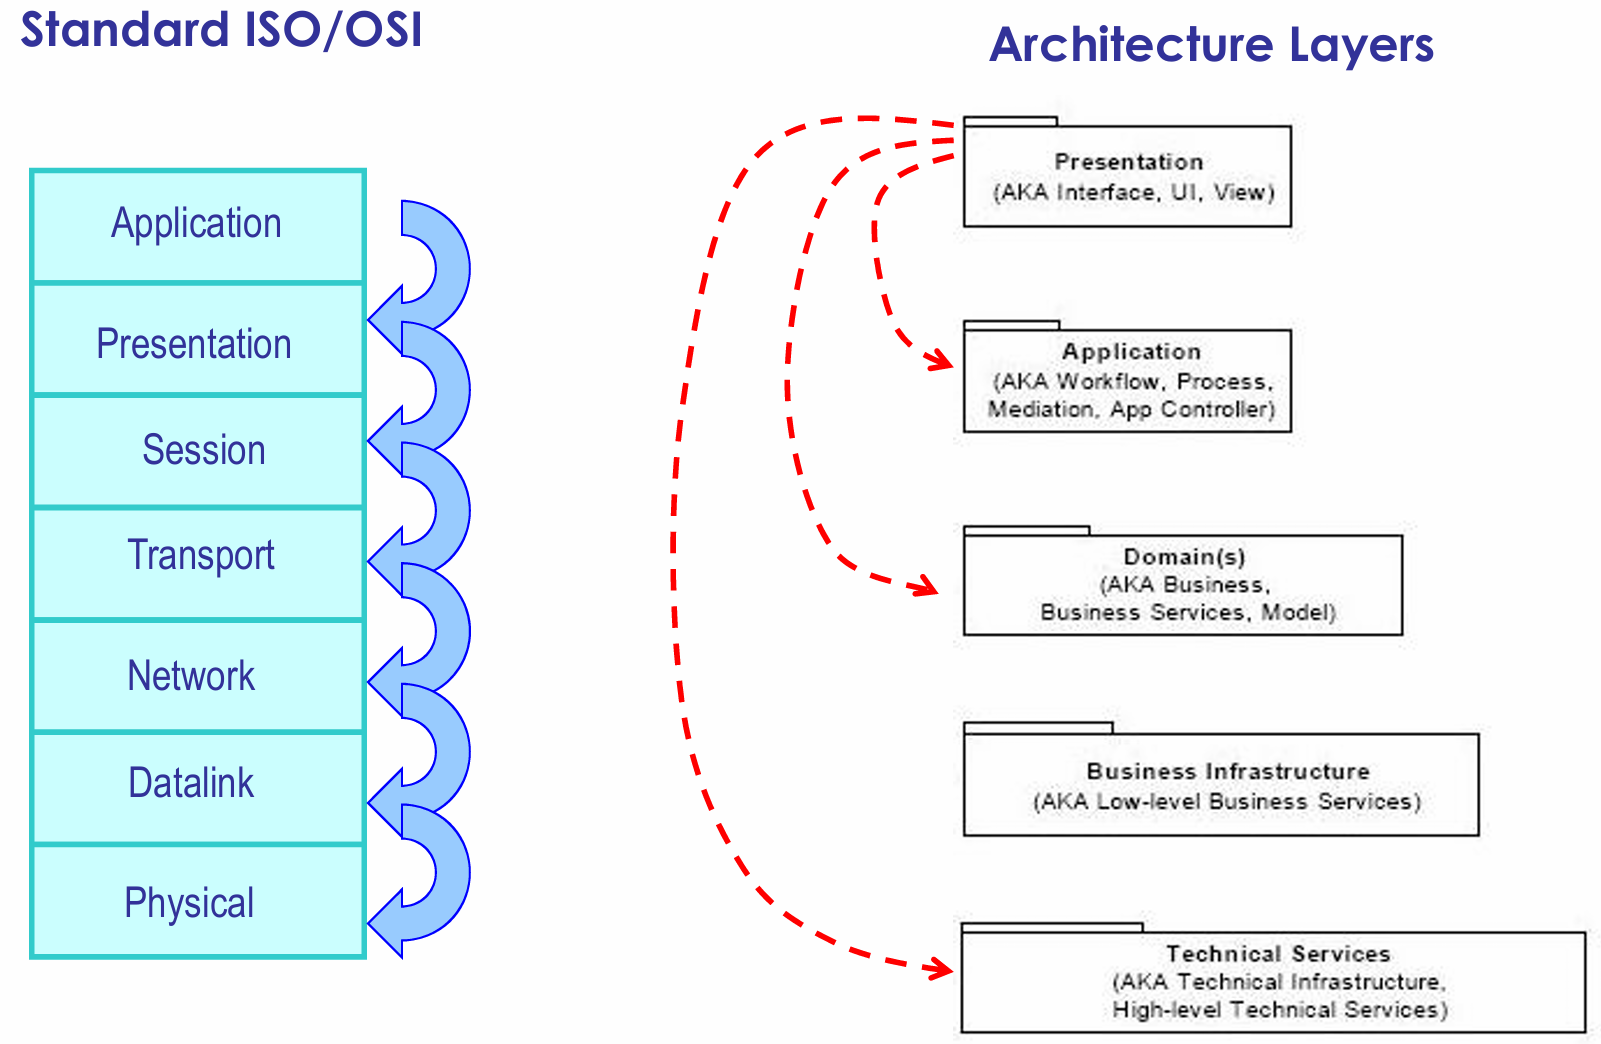
\includegraphics[scale=0.2]{architettura_layer/layer_rilassata.png}
    \end{center}

    \mysubsubsectionformatted{Layer sovrapposti}
    Alcuni oggetti appartengono univocamente a un solo layer.
    \\
    Può capitare che alcuni oggetti, invece, non siano facilmente classificabili, come ad esempio
    i layer Domain e Business Infrastructure oppure Technical Services e Foundation che possono essere
    uniti sotto nome di Infrastructure Layer.

    \newpage
    \mysubsubsectionformatted{Layers e partizioni}
    Generalmente:
    \begin{itemize}
        \item Layers: linee verticali.
        \item Partizioni: divisioni orizzontali.
    \end{itemize}
    Risulta utile distinguerli per diversi motivi:
    \begin{enumerate}
        \item Separation of concerns tra i servizi di alto e basso livello.
        \item Alcuni layers possono essere sostituiti nelle nuove implementazioni.
        \item I layer più bassi implementano funzionalità riutilizzabili.
        \item Viene favorito lo sviluppo in team dal momento che ciascuno sviluppatore è
              specializzato per un layer o servizio definito.
    \end{enumerate}

    \mysubsubsectionformatted{Architettura 3-tier}
    Tipo di architettura che divide il sistema in 3 componenti:
    \vspace{-0.5cm}
    \begin{center}
        \resizebox{\columnwidth}{!}{%
            \begin{tabular}{|l|l|}
                \hline
                \textbf{Interface}         & Interfaccia testuale, GUI e l'interazione diretta con l'utente \\ \hline
                \textbf{Application Logic} & Insieme dei task che governano i processi                      \\ \hline
                \textbf{Storage}           & Meccanismo di memorizzazione persistente (es. Database)        \\ \hline
            \end{tabular}%
        }
    \end{center}

    \begin{center}
        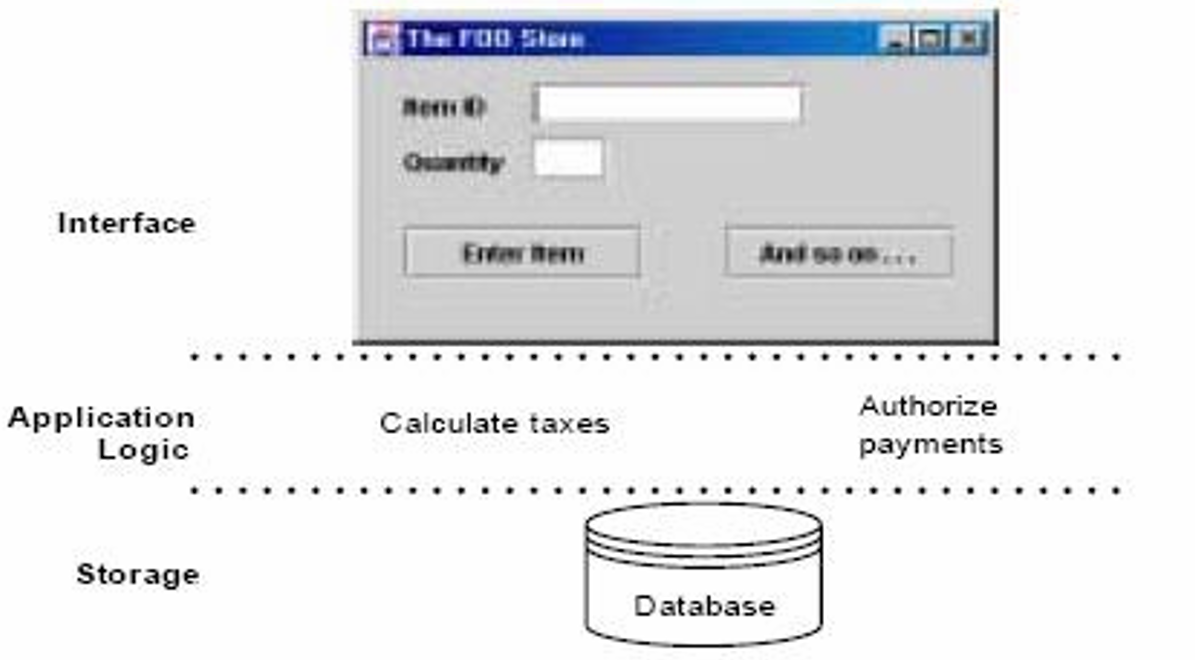
\includegraphics[scale=0.3]{architettura_layer/3tier_archi.png}
    \end{center}
    \newpage
}

\mysubsectionformatted{Design Principles e Design Patterns}
\myparagraph{
    In questa sezione si vanno ad analizzare i problemi che portano a un design
    inefficiente (Rotting Design).
    \\
    I sintomi sono i seguenti:
    \vspace{-0.5cm}
    \begin{center}
        \resizebox{\columnwidth}{!}{%
            \begin{tabular}{|
                    >{\columncolor[HTML]{3531FF}}l |l|}
                \hline
                {\color[HTML]{FFFFFF} \textbf{Rigidità}}   & \begin{tabular}[c]{@{}l@{}}Alta difficoltà nell'effettuare cambiamenti nel software, anche se si\\ tratta di cambiamenti semplici. Ogni cambiamento porta a sua volta la \\ necessità di cambiare ulteriori moduli dipendenti dal primo (effetto a cascata).\end{tabular}                                                                                    \\ \hline
                {\color[HTML]{FFFFFF} \textbf{Fragilità}}  & \begin{tabular}[c]{@{}l@{}}Tendenza del software di "rompersi" in seguito a dei cambiamenti nel software.\\ Spesso questi errori si verificano in aree che non hanno alcun collegamento\\ con l'area modificata.\end{tabular}                                                                                                                                \\ \hline
                {\color[HTML]{FFFFFF} \textbf{Immobilità}} & \begin{tabular}[c]{@{}l@{}}Non possibilità di riutilizzare il software da altri progetti oppure parti\\ dello stesso progetto.\end{tabular}                                                                                                                                                                                                                  \\ \hline
                {\color[HTML]{FFFFFF} \textbf{Viscosità}}  & \begin{tabular}[c]{@{}l@{}}Si distingue in viscosità del design e viscosità dell'ambiente (environment).\\ Il primo caso avviene se risulta facile commettere errori nel modificare il\\ design, a sua volta difficile nel fare le cose in modo corretto.\\ Il secondo caso avviene quando l'ambiente di sviluppo risulta lento e inefficiente.\end{tabular} \\ \hline
            \end{tabular}%
        }
    \end{center}
    Il fattore principale del perchè avvengono queste problematiche è dato dal fatto che al
    momento della creazione del design iniziale non vengono anticipati eventuali problemi.
    Il costante cambiamento delle parti del software porta a pensare che il design risulti
    inefficiente, quindi bisogna trovare un modo per renderlo più aperto al cambiamento.

    \mysubsubsectionformatted{Principi del Design Orientato agli Oggetti}
    \subsubsection{Open Closed Principle - OCP}
    \textit{Un modulo dovrebbe essere aperto alle estensioni ma chiuso per le modifiche}
    
    L'obiettivo di questo principio è garantire la creazione di moduli estendibili ma non senza modificare il codice sorgente.\\
    Si basa sulla tecnica dell'astrazione (in Java è abstract).
    
    \subsubsection{Liskov Substitution Principle - LSP}
    \textit{Le sottoclassi dovrebbero essere sostituibili per le loro classi base}
    
    L'obiettivo di questo principio è far sì che le classi derivate siano sostituibili per le loro classi padre. In questo modo,
    l'utente può continuare a usare le funzioni nonostante sia la classe derivata a essere passata (e non quella base).\\
    Sfortunatamente, qualora si violasse questo principio, risulterebbe difficile rilevare gli errori.
    
    \newpage
    \subsubsection{Dependency Inversion Principle - DIP}
    \textit{Si basa sull astrazione, non sulla concrezione}
    
    Questo principio si basa sull'uso delle interfacce o funzioni e classi astratte. Un'architettura orientata
    agli oggetti mostra una struttura dipendente dove la mggior parte delle dependency (relazioni) puntano verso
    le astrazioni. Nessuna dependency dovrebbe fare riferimento alle classi concrete. Il motivo è che gli oggetti concreti
    cambiano continuamente, quelli astratti meno frequentemente.
    
    \subsubsection{Interface Segregation Principle - ISP}
    \textit{Molte interfacce specifiche per gli utenti sono meglio di un'interfaccia generale}
    
    Se in una classe ci sono tanti clients, invece di caricare una classe con tutti i metodi richiesti dai clients, si
    creano delle interfacce specifiche per ciascuno. Nel caso più client necessitano dello stesso metodo, questo deve
    essere aggiunto in entrambi le interfacce.

    \mysubsubsectionformatted{Package Cohesion Principles}
    Sono utili per stabilire a quali package appartengono le classi.
    
    \subsubsection{Release Reuse Equivalency Principle - REP}
    \textit{La granulazione del riuso è la granulazione del rilascio}
    
    Spesso i client si rifiutano di utilizzare elementi a meno che gli autori non tengano traccia della versioni e
    mantengano le vecchie versioni per un po' di tempo. Quindi, un criterio per raggruppare le classi in un package è il riuso.
    Dal momento che i package sono delle unità di rilascio, a loro volta sono unità di riuso.
    
    \subsubsection{Common Closure Principle - CCP}
    \textit{Le classi che cambiano insieme sono inscindibili}
    
    Questo principio minimizza il numero di package che vengono cambiati per ogni rilascio del prodotto. Per far sì che
    questo principio funzioni, si raggruppano tutte quelle classi che pensiamo cambino insieme.
    
    \subsubsection{Common Reuse Principle - CRP}
    \textit{Classi che non vengono riusate insieme non dovrebbero essere raggruppate}

    Questo principio essenzialmente raggruppa quelle classi che non vengono usate insieme.
    
    \newpage
    \mysubsubsectionformatted{Package Coupling Principle}
    Questi principi governano le relazioni tra i package.
    \subsubsection{Acyclic Dependencies Principle - ADP}
    \textit{Le dipendenze tra i packages non devono creare dei cicli}

    Questo principio ha l'obiettivo di evitare la creazione di cicli, e quindi dipendenze cicliche, tra i package.
    L'eliminazione di un ciclo avviene in due modi, il primo consiste nel creare un nuovo package, il secondo è quello di
    usare i principi DIP e ISP.
    
    \subsubsection{Stable Dependencies Principle - SDP}
    \textit{Un modulo dovrebbe dipendere solo da moduli più stabili di lui}
    
    Quando si parla di \textit{stabilità} si intende il quantitativo di lavoro richiesto per effetturare una modifica.
    Esistono tanti fattori che rendono un software difficile da modificare (complessità, dimensione, chiarezza ecc\dots), ma
    fattori più importante è il fatto che tanti package software dipendano da uno solo.
    
    Esistono delle \coloredtext[blue]{\textbf{Metriche di Stabilità}} per semplificare le modifiche.
    \begin{center}
        \resizebox{\columnwidth}{!}{%
            \begin{tabular}{|
                    >{\columncolor[HTML]{3166FF}}l |l|}
                \hline
                {\color[HTML]{FFFFFF} \textbf{Ca - Afferent Coupling}} & \begin{tabular}[c]{@{}l@{}}Numero di classi fuori dal package che dipende dalle\\ classi dentro al package.\end{tabular}                 \\ \hline
                {\color[HTML]{FFFFFF} \textbf{Ce - Efferent Coupling}} & \begin{tabular}[c]{@{}l@{}}Numero di classi fuori dal package dipese dalle\\ classi dentro al package.\end{tabular}                      \\ \hline
                {\color[HTML]{FFFFFF} \textbf{I - Instability}}        & \begin{tabular}[c]{@{}l@{}}$I = \frac{Ce}{Ca + Ce}$\\ Se I = 0, il package è stabile,\\ altrimenti I = 1 ed è instabile.\end{tabular} \\ \hline
            \end{tabular}%
        }
    \end{center}

    \subsubsection{Stable Abstraction Principle - SAP}
    \textit{Package stabili dovrebbero essere astratti}
    \\
    Solitamente, una struttura di package prevede che quelli più in alto siano instabili e flessibili (facili da cambiare),
    mentre quelli più in basso sono difficili da cambiare per la loro stabilità.
    \\
    Un modo per rendere più semplice la modifica avviene tramite \coloredtext[blue]{\textbf{Metriche di Astrazione}}:
    \vspace{0.1cm}
    \begin{center}
        \resizebox{0.7\columnwidth}{!}{%
            \begin{tabular}{|
                    >{\columncolor[HTML]{3166FF}}l |l|}
                \hline
                {\color[HTML]{FFFFFF} \textbf{Nc}} & Numero di classi nel package.                                                                                                                                                 \\ \hline
                {\color[HTML]{FFFFFF} \textbf{Na}} & Numero di classi astratte nel package                                                                                                                                         \\ \hline
                {\color[HTML]{FFFFFF} \textbf{A}}  & \begin{tabular}[c]{@{}l@{}}Astrazioni, $A = \frac{Na}{Nc}$\\ Se A = 0, il package non ha classi astratte,\\ altrimenti A = 1 e contiene classi astratte.\end{tabular} \\ \hline
            \end{tabular}%
        }
    \end{center}

    \newpage
    Adesso possiamo confrontare le due metriche \textit{I} e \textit{A}. La metrica \textit{I} dovrebbe incrementare mentre
    \textit{A} decrementa, in questo modo, i package concreti dovrebbero essere instabili mentre quelli astratti dovrebbero
    essere stabili.
    \begin{center}
        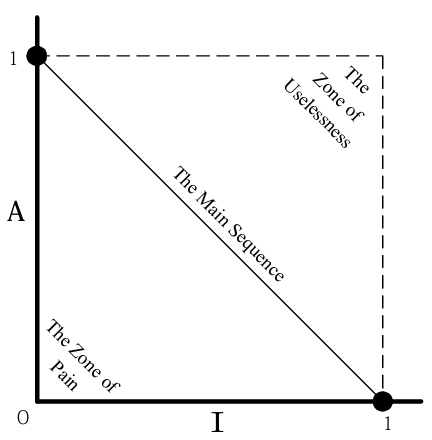
\includegraphics[scale=0.5]{design_principles_design_patterns/Grafo_AvsI.jpeg}
    \end{center}
    Nel grafico, in alto a sinistra troviamo i package astratti e stabili, in basso a destra i package concreti e instabili.
    \\
    Altre metriche utili sono le \coloredtext[blue]{\textbf{Metriche di Distanza}}, utili per stabilire quanto è lontano
    un package dalla \textit{main sequence}, ovvero la distanza massima tra i package concreti e quell astratti.
    \begin{center}
        \resizebox{\columnwidth}{!}{%
            \begin{tabular}{|
                    >{\columncolor[HTML]{3166FF}}l |l|}
                \hline
                {\color[HTML]{FFFFFF} \textbf{D - Distance}}             & $D = \frac{|A + I - 1|}{\sqrt{2}}$ \\ \hline
                {\color[HTML]{FFFFFF} \textbf{D' - Normalized Distance}} & \begin{tabular}[c]{@{}l@{}}$D' = |A + I - 1|$\\ Se D' = 0, il package è nella main sequence,\\ se D' = 1, è il più lontano possibile.\end{tabular} \\ \hline
            \end{tabular}%
        }
    \end{center}
    \newpage

}

\mysubsectionformatted{Pattern of Enterprise Applications Architectures}
\myparagraph{
    All'interno di grandi aziende, si hanno una grandissima quantità di dati da gestire,
    organizzati in sistemi moderni come i DBMS, e nel tempo questi dati potranno dover essere
    migrati attraverso nuove applicazioni, si parla di dati persistenti su archi di tempo molto ampi.
    \\
    L'accesso a questi dati è concorrente, arrivando fino a milioni di accessi contemporanei, le interfacce
    sono molto articolate, distinte tra loro e presentate in modo differente per tipi di utenti e obiettivi
    differenti.
    \\
    Le applicazioni \textbf{enterprise} possono essere integrate con ulteriori applicazioni. Queste fanno uso
    di architetture stratificate (per la maggior parte di essi).
    
    \coloredtext[blue]{\textbf{Business Logic:}} regole di interpretazione e elaborazione dei dati in base
    all'utilità dell'applicazione. Queste regole tendono a cambiare in base a diversi criteri:
    \begin{itemize}
        \item Gestione personalizzata di clienti
        \item Adeguamento a nuove logiche di mercato
        \item Cambiamento nelle strategie di marketing
        \item Altro
    \end{itemize}

    Riguardo la \textbf{performance}, molte decisioni architetturali aggravano su essa, portando a sacrificarne
    un po' pur di migliorare la comprensibilità.\\
    Tra i fattori che costituiscono la performance abbiamo la \textbf{scalabillità},
    \\l'\textbf{efficienza}, il \textbf{Tempo di Risposta} e la \textbf{Latenza} (Quanto puoi fare in un certo lasso di tempo).
    
    \mysubsubsectionformatted{Design Patterns e Architetturali}
    Per fare una distinzione tra i due:
    \begin{tcolorbox}[colback=blue!5!white, colframe=blue!75!black]
        I \textbf{Design Pattern} aiutano a trovare delle soluzioni a problemi in modo tale che si possano usare queste soluzioni
        tantissime volte. Purtroppo adattarli ai casi reali richiede uno sforzo progettuale significativo.
    \end{tcolorbox}

    \begin{tcolorbox}[colback=green!5!white, colframe=green!75!black]
        I \textbf{Pattern Architetturali} offrono soluzioni a problemi architetturali, aiutando a documentare le decisioni prese,
        facilitando la comunicazione tra gli stakeholder mediante un vocabolario comune.
    \end{tcolorbox}
    \newpage
    \mysubsubsectionformatted{Tipologie di Pattern Architetturali}
    \begin{enumerate}
        \item Domain Logic Patterns
        \item Data Source Architectural Patterns
        \item Object Relational Behavioral Patterns
        \item Object Relational Structural Patterns
        \item Web Presentation Patterns
        \item Concurrency Patterns
        \item Security Patterns
              \begin{enumerate}
                \renewcommand{\labelenumii}{\theenumi.\arabic{enumii}}
                \setcounter{enumii}{0}
                  \item Federated Identity Pattern
                  \item Gatekeeper Pattern
                  \item Valet Key Pattern
              \end{enumerate}
        \item Performance Patterns
    \end{enumerate}
    Per descrivere un pattern architetturale ci focalizzeremo su 4 punti:
    \begin{enumerate}
        \item \textbf{Descrizione}
        \item \textbf{Diagramma UML}
        \item \textbf{Esempio di applicazione}
        \item \textbf{Vantaggi e Svantaggi}
    \end{enumerate}
    \mysubsubsectionformatted{Frameworks}
    I framework sono delle librerie di codice astratte e estendibili che vengono adattate per scopi specifici da parte
    degli sviluppatori. Per i software moderni sono oramai essenziali, migliorano la produttività ma con degli effetti
    collaterali indesiderati, come debolezze architetturali o vulnerabilità nella sicurezza.
    \\
    Tra i framework più conosciuti abbiamo
    \begin{itemize}
        \item Maven
        \item Django
        \item Spring
        \item Molti altri
    \end{itemize}

    Tra i produttori di framework troviamo anche \textbf{Amazon Web Services (AWS)} e \textbf{Microsoft's Azure}.
    
    \newpage
}

\mysubsectionformatted{Web Presentation Patterns}
\myparagraph{
Generalmente, sono quei pattern volti alla definizione dell'interfaccia utente.
Tra le tecnologie e i framework che fa uso questo tipo di pattern abbiamo:
\begin{itemize}
    \item Java Servlet
    \item Server pages (JSP, PHP, ASP)
    \item Apache XAlan
    \item Altro
\end{itemize}
I Web Presentation Patterns si dividono in due categorie:
\begin{enumerate}
    \item \textbf{Model-view-controller}
    \begin{enumerate}
        \item Controller Design
        \begin{enumerate}
            \item Page Controller
            \item Front Controller
            \item Intercepting Filter
        \end{enumerate}
        \item View Design
        \begin{enumerate}
            \item Template view
            \item Transformation view
            \item Two-step view
        \end{enumerate}
    \end{enumerate}
    \item \textbf{Application Controller}
\end{enumerate}
}
\newpage

\mysectionformatted{Metriche, Understand, Refactoring e Antipattern strutturali}
\mysubsectionformatted{Metriche Object Oriented}
\myparagraph{
    Nei sistemi Object Oriented, per gestire casi come Polimorfismo, Ereditarietà,
    Information hiding e Astrazione, vengono usate delle metriche apposite in base al
    criterio che vogliamo verificare.
    \\
    Le metriche sono:
    \begin{enumerate}
        \item \textbf{Line of code per class}
        \item \textbf{Weighted method per class}
        \item \textbf{Depth of the inheritance tree}
        \item \textbf{Number of children}
        \item \textbf{Coupling between object classes}
        \item \textbf{Response for a class}
        \item \textbf{Lack of cohesion in methods}
    \end{enumerate}

    \mysubsubsectionformatted{Line of code per class (LOCC)}
    Calcola quante linee di codice ci sono in un metodo.

    Sia:
    \begin{enumerate}
        \item \textit{c} la classe che si sta valutando
        \item \textit{LOC(m)} il numero di linee nel metodo \textit{m}
        \item \(\textit{M}_{\textit{Im}} (c)\) insieme dei metodi implementati nella classe \textit{c}
    \end{enumerate}
    
    La formula per calcolare le linee di codice nella classe è
    \vspace{-1cm}
    \begin{center}
        \begin{equation}
            LOCC(c) = \sum_{m \in M_{Im} (c)} LOC(m)
        \end{equation}
    \end{center}
    
    \newpage
    \mysubsubsectionformatted{Weighted method per class (WMC)}
    Calcola il livello di complessità dei metodi in una classe.
    Sia:
    \begin{enumerate}
        \item \textit{c} la classe che si sta valutando
        \item \textit{VG(m)} la complessità ciclomatica del metodo \textit{m}
        \item \(\textit{M}_{\textit{Im}} (c)\) insieme dei metodi implementati nella classe \textit{c}
    \end{enumerate}
    La formula per calcolare la complessità di una classe (o complessità di McCabe) è
    \vspace{-1cm}
    \begin{center}
        \begin{equation}
            WMC(c) = \sum_{m \in M_{Im} (c)} VG(m)
        \end{equation}
    \end{center}
    \`{E} una metrica importante, in quanto stabilisce l'indice di complessità di una classe, quindi quanto sia comprensibile
    e facile da modificare.\\
    Maggiore è il numero dei metodi, maggiore è la complessità della classe\\ \Rightarrow maggiore è la probabilità
    che la classe è legata all'applicazione\\ \Rightarrow minore possibilità di riuso.

    \mysubsubsectionformatted{Depth of the inheritance tree (DIT)}
    Calcola la distanza massima di un nodo dalla radice dell'albero. In altre parole verifica quanto una classe
    venga ereditata da altre classi.
    \begin{itemize}
        \item Maggiore è la profondità della classe, maggiore è il numero di metodi che essa può ereditare, rendendo più 
        complesso predire il suo comportamento.
        \item Alberi di ereditarietà con maggiore profondità aumentano la complessità del progetto, dato che più classi e
        metodi sono coinvolti.
        \item Maggiore è la profondità di una classe in una gerarchia, maggiore è il riuso potenziale dei metodi ereditati.
    \end{itemize}

    \mysubsubsectionformatted{Number of children (NOC)}
    Calcola il numero di sottoclassi di una superclasse.\\
    Al crescere del numero di sottoclassi si verificano i seguenti casi:
    \begin{itemize}
        \item Cresce il livello di riuso.
        \item Aumenta la quantità di test case necessari a testare ogni superclasse.
        \item La superclasse tende a diventare impertinente, perchè ciascuna sottoclasse può 
        aggiungere dei comportamenti specifici ai metodi, distaccandosi \\dall'idea generale della superclasse. 
        \item Le sottoclassi potrebbero non essere membri appropriati della madre, perchè può accadere che la sottoclasse
        erediti dei metodi che non ritiene sensato usare.
    \end{itemize}

    \mysubsubsectionformatted{Coupling between object classes (CBO)}
    Calcola il numero di classi a cui una classe è accoppiata.\\
    Un eccessivo accoppiamento è sicuramente negativo in termini di modularità e riuso, infatti si consiglia sempre
    di mantenere un basso accoppiamento (low coupling) in modo da facilitare test e modifiche.

    \mysubsubsectionformatted{Response for a class (RFC)}
    Calcola l'insieme dei metodi che possono essere eseguiti in risposta ad un messaggio ricevuto da un oggetto della classe.\\
    Un elevato numero di metodi può aumentare la complessità progettuale della classe e lo sforzo dei test.

    \mysubsubsectionformatted{Lack of cohesion in methods (LCOM)}
    Calcola la non-coesione tra gli elementi di una classe. Viene espressa tramite numero di metodi che accedono agli 
    stessi attributi di una classe.
    
    Sia:
    \begin{enumerate}
        \item \textit{C} una classe con \textit{n} metodi \textit{\(M_1, M_2,\dots M_n\)}
        \item \textit{\(I_j\)} l'insieme delle istanze di variabili referenziate da \textit{\(M_i\)}
        \item \textit{\(P = \{(I_j, I_i) \mid I_i \cap I_j = \varnothing \}\)}
        \item \textit{\(Q = \{(I_j, I_i) \mid I_i \cap I_j \neq  \varnothing \}\)}
    \end{enumerate}
    Presi tutti gli insiemi \(I_1 , \dots I_n \), se sono vuoti allora P = \varnothing.
    \vspace{-0.1cm}
    \begin{center}
               \textit{se |P| > |Q| allora LCOM = |P| - |Q|, altrimenti LCOM = 0}
    \end{center}
    Quindi \textit{LCOM = num. intersezioni vuote - num. intersezioni non vuote}\\
    Minore è il valore di LCOM, maggiore è la coesione (metodi strettamente legati tra loro e la classe ha uno scopo chiaro).\\
    Maggiore è il valore di LCOM, minore è la coesione (i metodi non condividono molti attributi comuni, quindi la classe è
    più difficile da gestire e comprendere).
    \begin{itemize}
        \item \`E sempre consigliato avere una classe altamente coesa, in modo da favorirne la sua incapsulazione.
        \item Una bassa coesione può comportare una divisione di una classe in due o più sottoclassi.
        \item Una bassa coesione comporta anche complessità e probabilità di compiere errori durante il processo di sviluppo.
    \end{itemize}
    \newpage
    Ultima considerazione riguardo a questa metrica, esiste un altro metodo proposto da Henderson-Sellers che, tramite una formula
    (che non starò a scrivere), ci indica se la coesione è perfetta o meno:
    \begin{itemize}
        \item Se \textbf{LCOM = 0}, la coesione è perfetta (tutti gli attrbiuti sono acceduti da tutti i metodi della classe).
        \item Se \textbf{LCOM = 1}, c'è una completa mancanza di coesione (ogni attributo è acceduto da un solo metodo della classe).
    \end{itemize}

    \newpage
}

\mysectionformatted{Esercitazioni}
\myparagraph{
    In questo capitolo, vengono analizzati dei design pattern nuovi e non trattati
    durante il corso di Analisi e Progettazione.
    Verrà fatto anche qualche riferimento a pattern già visti.

    \begin{tcolorbox}[colback=red!5!white, colframe=red!75!black]
        \textbf{Attenzione}, il file fornito chiarisce solo le nozioni teoriche sui pattern trattati, per
        approfondirli in maniera pratica si consigliano le slide fornite dai professori (e ovviamente testare
        su codice il loro funzionamento).
    \end{tcolorbox}
}

\mysubsectionformatted{Design Pattern State}
\myparagraph{

    \begin{tcolorbox}[colback=blue!5!white, colframe=blue!75!black]
        Permette a un oggetto di modificare il suo comportamento quando il suo
        stato interno cambia.
    \end{tcolorbox}

    \noindent\textit{State} viene utilizzato quando si vuole modificare lo stato interno di un oggetto
    in modo da potergli far eseguire determinati metodi. Gli stati degli oggetti vengono rappresentati
    da classi differenti che estendono una classe astratta che rappresenta lo stato dell'oggetto.

    \begin{center}
        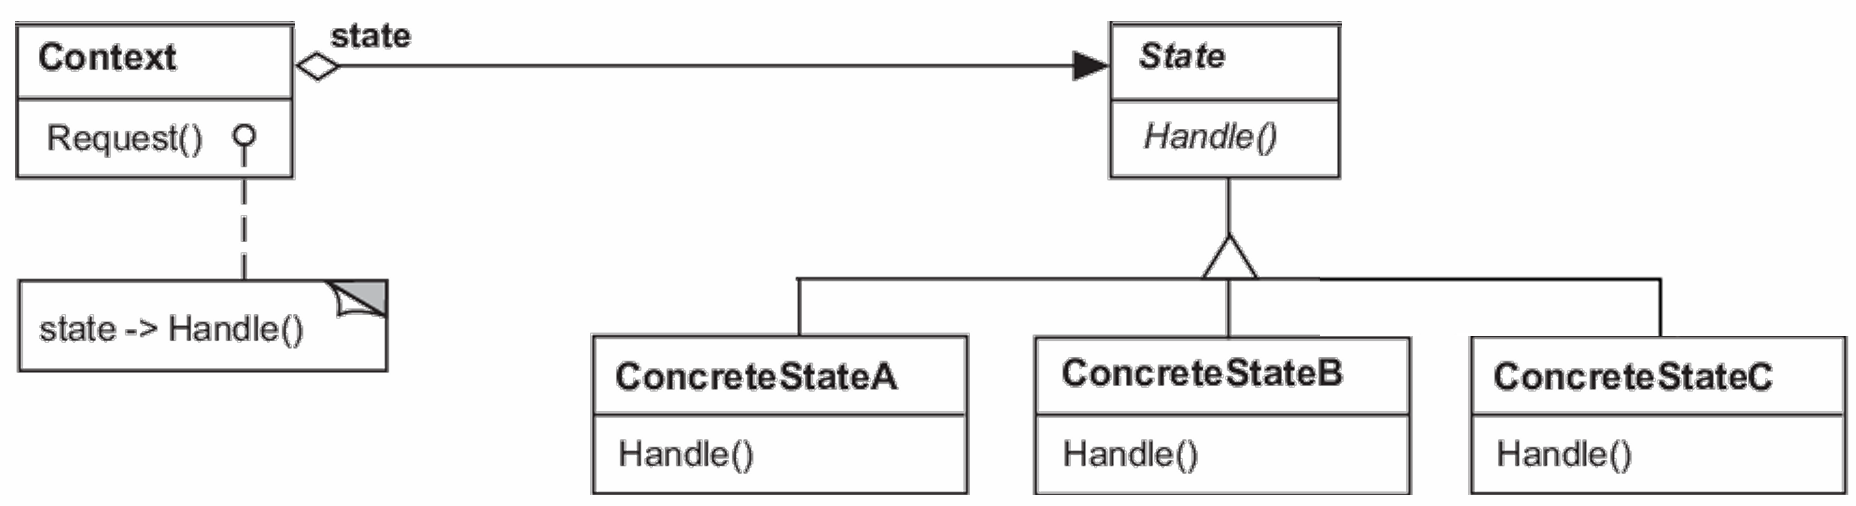
\includegraphics[scale=0.25]{Esercitazione - Design Patterns/state_pattern.png}
    \end{center}

    \begin{enumerate}
        \item \textbf{Context} è l'interfaccia del client. Ha un'istanza di \textbf{ConcreteState} che indica in che stato si trova.
        \item \textbf{\textit{State}} è la classe astratta che rappresenta lo stato attuale di \textbf{Context}.
        \item \textbf{ConcreteState} sono le classi che implementano il comportamento \\associato allo stato del \textbf{Context}.
    \end{enumerate}

    \begin{center}
        \resizebox{\columnwidth}{!}{%
            \begin{tabular}{|l|l}
                \hline
                \rowcolor[HTML]{32CB00}
                \multicolumn{1}{|c|}{\cellcolor[HTML]{32CB00}\textbf{Vantaggi}}                                                                       & \multicolumn{1}{c|}{\cellcolor[HTML]{FE0000}\textbf{Svantaggi}} \\ \hline
                Eliminazione di tanti "if"                                                                                                            & \multicolumn{1}{l|}{Incremento del numero di oggetti}           \\ \hline
                Facile lettura del codice                                                                                                             & \multicolumn{1}{l|}{Richiede la scrittura di molto codice}      \\ \hline
                \begin{tabular}[c]{@{}l@{}}Nuovi stati e transizioni possono essere\\ aggiunti facilmente definendo nuove \\ sottoclassi\end{tabular} &                                                                 \\ \cline{1-1}
            \end{tabular}%
        }
    \end{center}

    \newpage
    \subsubsection{Esempio di Pattern State}
    \begin{center}
        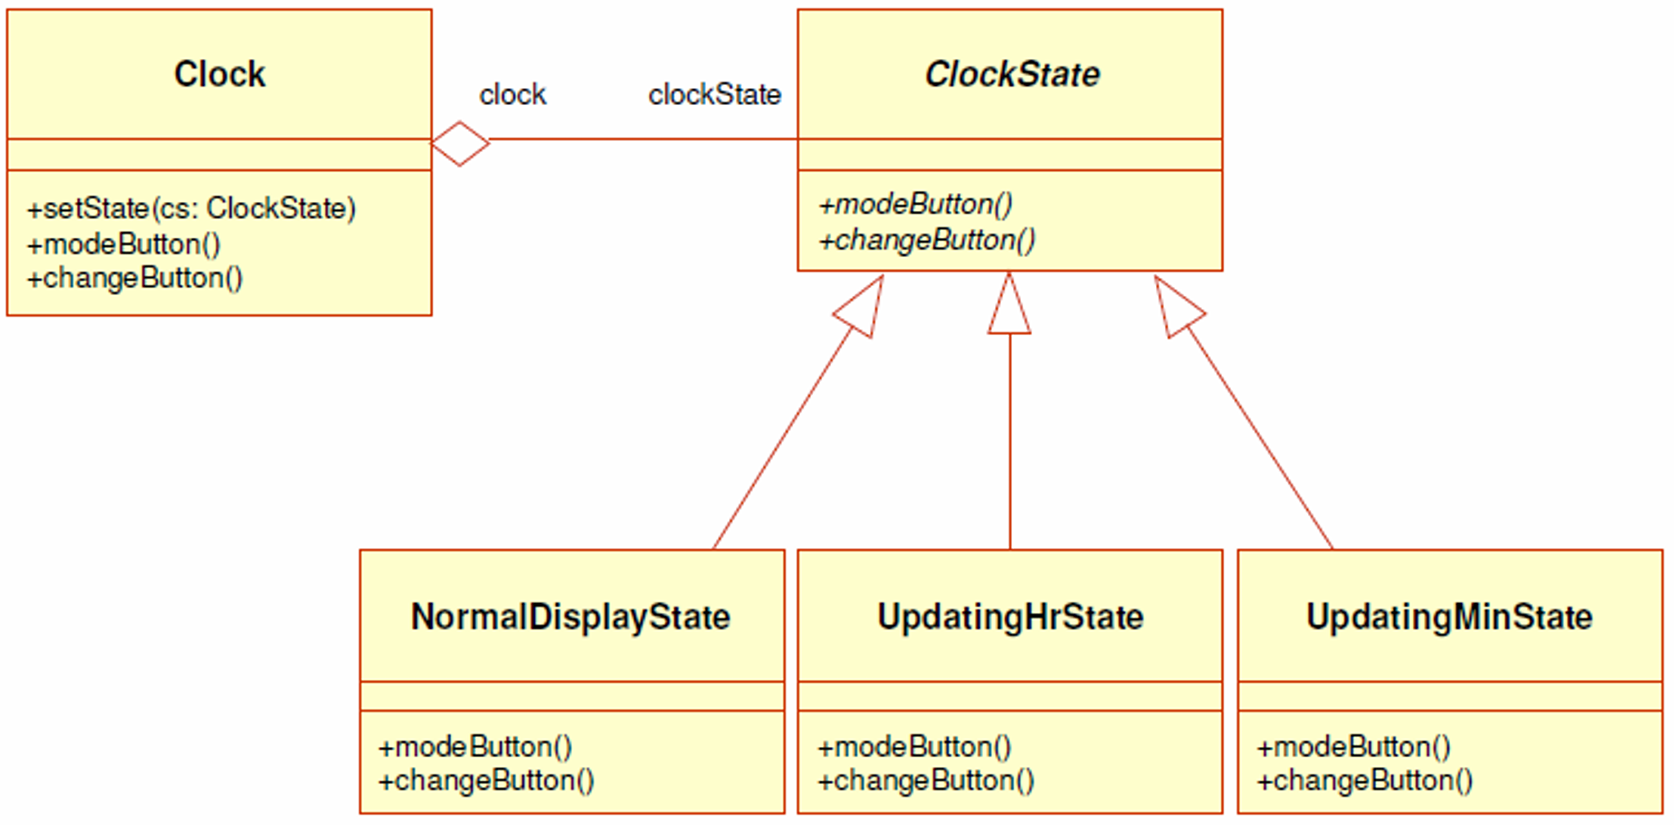
\includegraphics[scale=0.25]{Esercitazione - Design Patterns/example_state_pattern.png}
    \end{center}
    In questo esempio, \textbf{Clock} contiene 3 metodi di cui \textbf{modeButton()} e \textbf{changeButton()} cambiano il loro
    comportamento in base allo stato in cui si trova. \textbf{setState(cs: ClockState)} permette di cambiare lo stato di \textbf{Clock},
    in questo modo, anche i due metodi all'interno cambieranno il loro comportamento.

    \mysubsubsectionformatted{State vs Strategy}
    Sono entrambi pattern comportamentali, ma hanno obiettivi e applicazioni \\differenti.

    \begin{tcolorbox}[colback=blue!5!white, colframe=blue!75!black]
        State cambia il comportamento di un oggetto in base al suo stato interno.
        \\Es. Un lettore audio che può avere stati come "Play", "Pause" e "Stop", dove ogni stato 
        gestisce le azioni dell'utente in modo diverso.
    \end{tcolorbox}

    \begin{tcolorbox}[colback=green!5!white, colframe=green!75!black]
        Strategy consente di cambiare il modo in cui un'operazione viene eseguita, senza modificare lo stato interno dell'oggetto.
        \\Es. Un sistema di pagamento che può usare diverse strategie come "Carta di credito", "PayPal" o "Bonifico", a seconda della scelta dell'utente.
    \end{tcolorbox}
    \newpage

}

\mysubsectionformatted{Design Pattern Command}
\myparagraph{

    \begin{tcolorbox}[colback=blue!5!white, colframe=blue!75!black]
        Permette di trasformare una richiesta in un oggetto indipendente.
        \\In questo modo si possono:
        \begin{enumerate}
            \item scollegare il mittende di una richiesta dal destinatario.
            \item rendere le operazioni riutilizzabili.
            \item registrare e annullare operazioni.
            \item creare sequenze di comandi.
        \end{enumerate}
    \end{tcolorbox}
    \noindent\textit{Command} è ideale per implementare operazioni complesse e modulari
    che possono essere facilmente eseguite, annullate, memorizzate e organizzate in sequenza.

    \begin{center}
        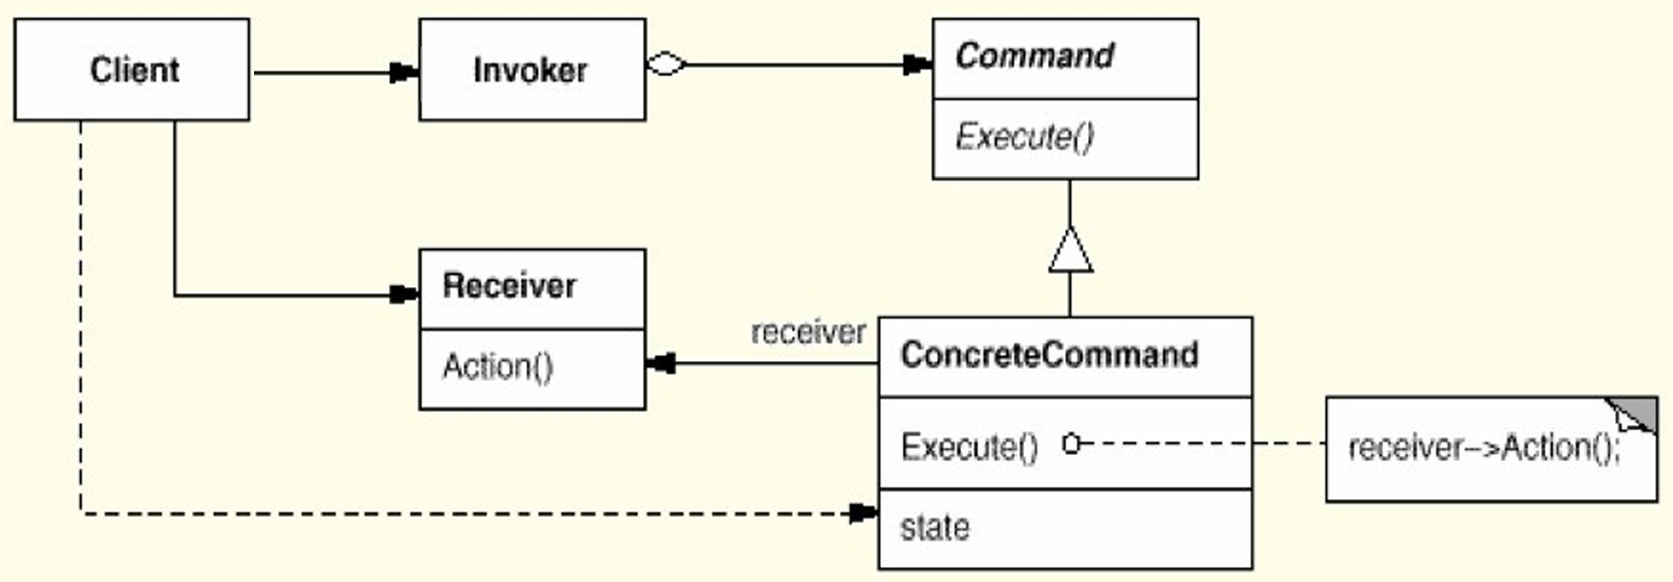
\includegraphics[scale=0.25]{Esercitazione - Design Patterns/command_pattern.png}
    \end{center}

    \begin{enumerate}
        \item \textbf{Client} è l'interfaccia che crea un'istanza concreta  \textbf{ConcreteCommmand}
              e ne imposta il \textbf{Receiver}.
        \item \textbf{\textit{Command}} è l'interfaccia per l'esecuzione dell'operazione.
        \item \textbf{ConcreteCommand} è la classe che incapsula l'operazione da eseguire
              in un oggetto specifico.
        \item \textbf{Invoker} è la classe che che richiede tramite il \textbf{\textit{Command}}
              l'esecuzione di una o più operazioni.
        \item \textbf{Receiver} è l'oggetto che esegue l'azione.
    \end{enumerate}

    \begin{center}
        \resizebox{\columnwidth}{!}{%
            \begin{tabular}{|l|}
                \hline
                \rowcolor[HTML]{32CB00}
                \multicolumn{1}{|c|}{\cellcolor[HTML]{32CB00}\textbf{Vantaggi}}                                                                                \\ \hline
                Separa l'oggetto che invoca l'operazione da quello che sa come eseguirlo                                                                       \\ \hline
                \begin{tabular}[c]{@{}l@{}}I \textit{Command} sono classi di oggetti e possono essere manipolati \\ come qualsiasi altro oggetto.\end{tabular} \\ \hline
                Si possono creare dei \textit{Command} composti.                                                                                               \\ \hline
                \'E semplice aggiungere nuovi \textit{Command}.                                                                                                \\ \hline
            \end{tabular}%
        }
    \end{center}
    \newpage
    \subsubsection{Esempio di Design Pattern Command}
    \begin{center}
        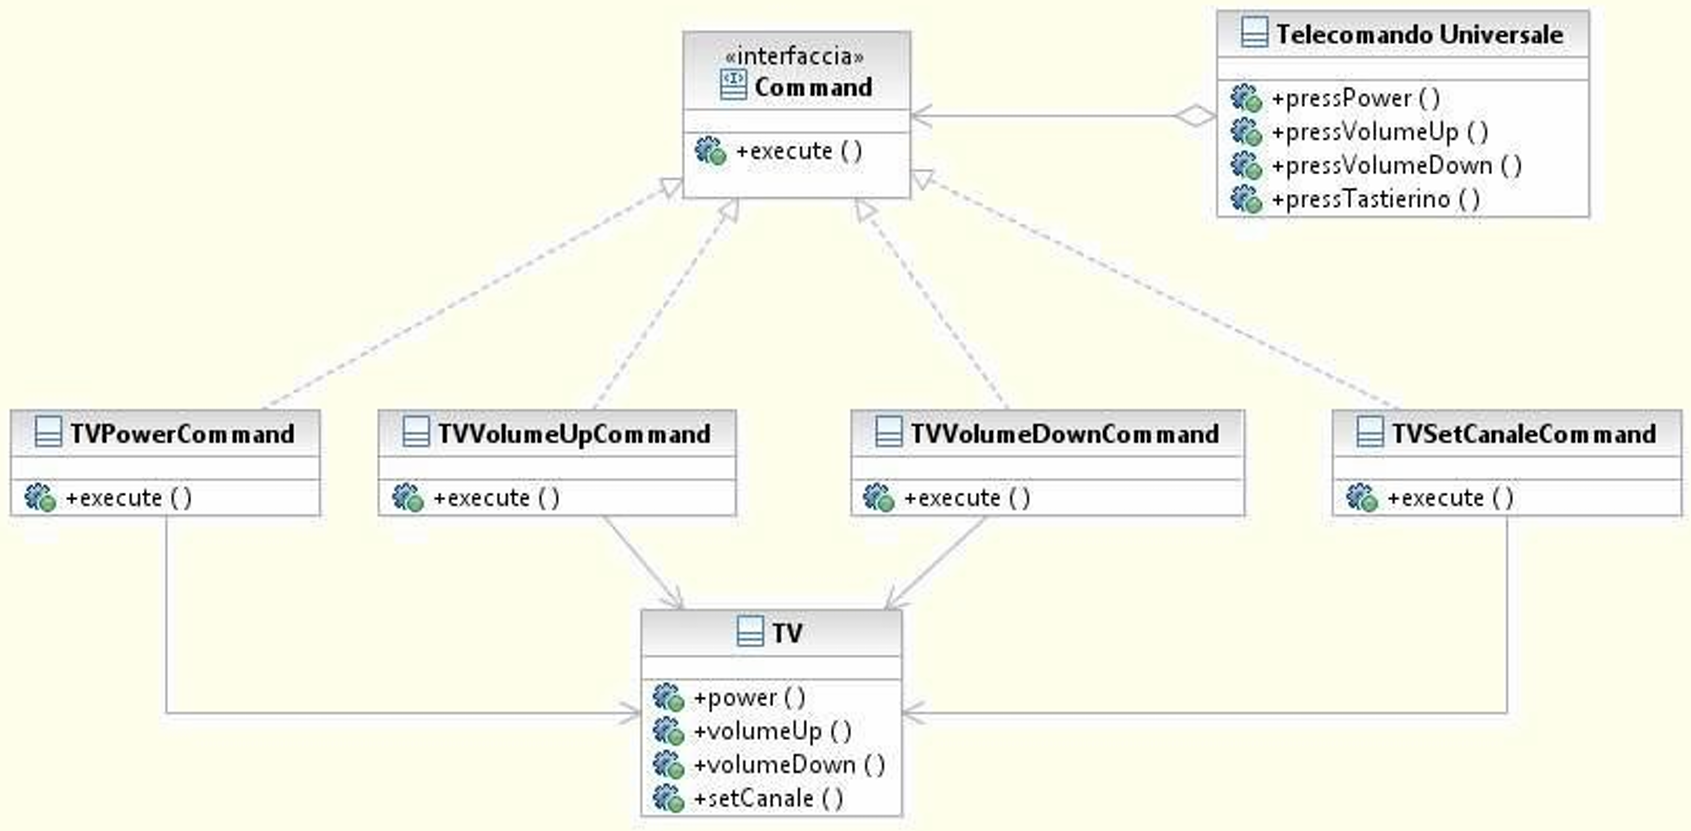
\includegraphics[scale=0.26]{Esercitazione - Design Patterns/example_command_pattern.png}
    \end{center}
    In questo esempio, \textbf{TV} è il \textbf{Receiver} che esegue l'azione stabilita dal \textbf{Telecomando Universale},
    ovvero l'\textbf{Invoker}. 
    \\
    I \textbf{ConcreteCommand} sono le 4 classi che ereditano il metodo \textbf{execute()} che
    invocano le corrispondenti operazioni del \textbf{Receiver}.
    \\
    Infine l'interfaccia \textbf{\textit{Command}} che definisce l'interfaccia alle classi concrete.
    \newpage

}

\mysubsectionformatted{Design Pattern Template}
\myparagraph{

    \begin{tcolorbox}[colback=blue!5!white, colframe=blue!75!black]
        Definisce lo scheletro in un'operazione, lasciando alle sottoclassi di \\modificare
        l'algoritmo senza cambiare la sua struttura.
    \end{tcolorbox}
    \noindent Usiamo \textit{Template} quando si vuole implementare le invarianti di un algoritmo una sola volta,
    saranno le sottoclassi a implementare le varie varianti.

    \subsubsection{Struttura del pattern Template}
    \begin{center}
        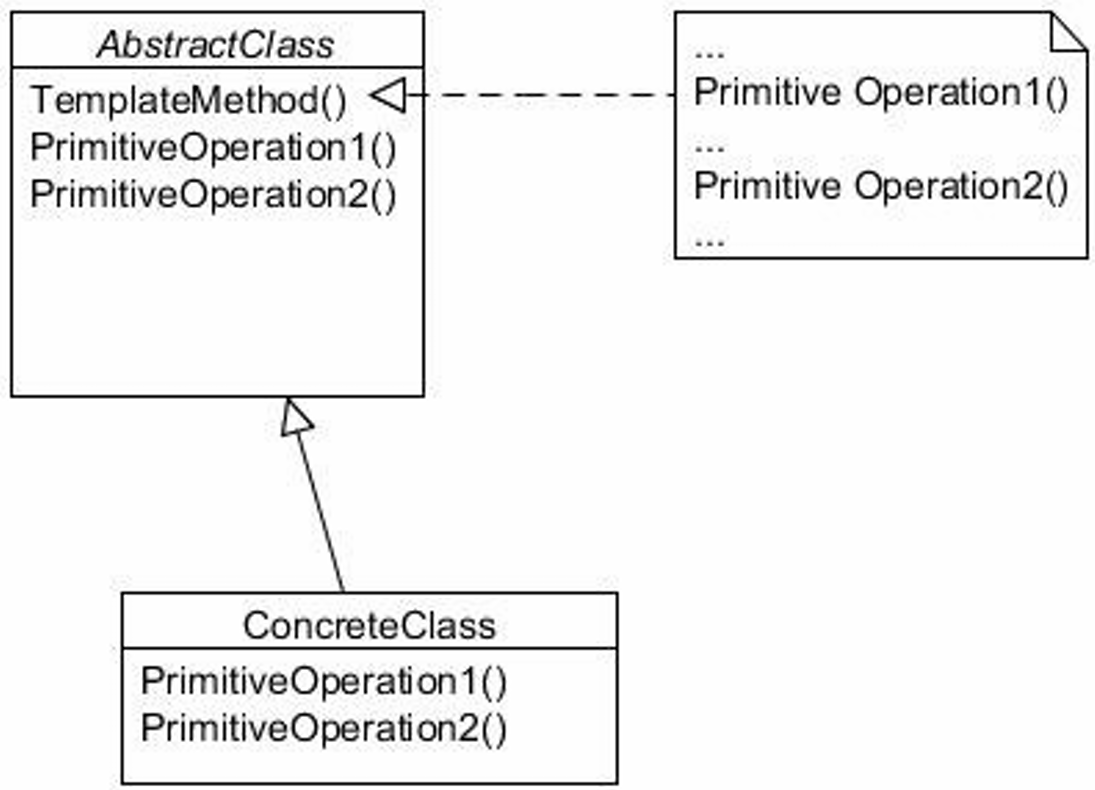
\includegraphics[scale=0.25]{Esercitazione - Design Patterns/template_pattern.png}
    \end{center}
    \begin{enumerate}
        \item \textit{\textbf{AbstractClass}} è la classe che definisce le operazioni primitive di tipo astratto.
        Queste vengono poi implementate dalle sottoclassi \textbf{ConcreteClass}. Definisce un metodo \textbf{TemplateMethod()}
        che rappresenta lo scheletro di un algoritmo e richiama le operazioni primitive.
        \item \textbf{ConcreteClass} sono le classi che implementano le operazioni primitive per poterne variare il 
        comportamento.
    \end{enumerate}
    I metodi template sono fondamentali per il riutilizzo del codice, soprattutto nelle librerie di classi, questo perchè
    sono i mezzi per estrapolare i comportamenti comuni in classi di libreria. Bisogna sempre specificare quali operazione 
    si vogliono sovrascrivere e quali metodi trasferiti alle sottoclassi.

    \newpage
    \subsubsection{Esempio di Design Pattern Template}
    \begin{center}
        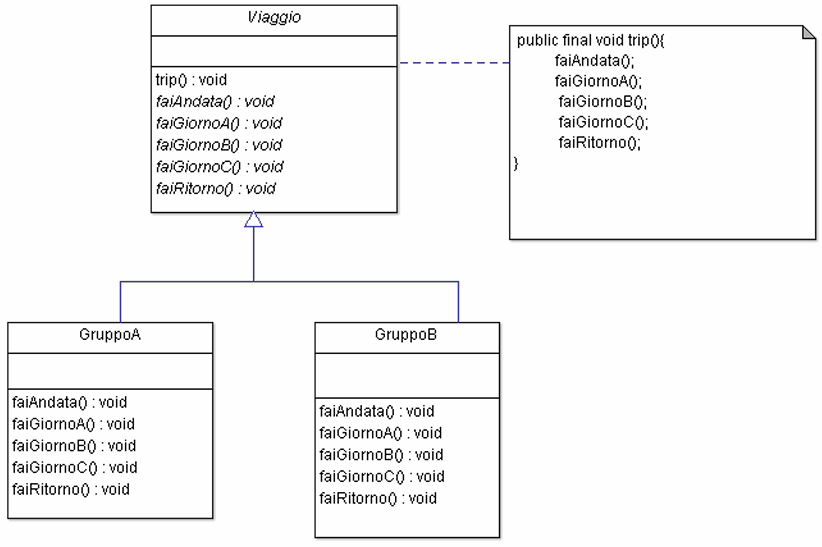
\includegraphics[scale=0.5]{Esercitazione - Design Patterns/example_template_pattern.png}
    \end{center}
    In questo esempio, \textit{Viaggio} è l'\textit{\textbf{AbstractClass}} che contiene il metodo Template \textbf{trip()}. Le
    \textbf{ConcreteClass} \textbf{GruppoA} e \textbf{GruppoB} ereditano i metodi dalla superclasse, decidendo però come deve essere
    implementato ciascun metodo.

    \newpage
}

\mysubsectionformatted{Design Pattern Repository}
\myparagraph{
    Questo design pattern viene usato se, ad esempio, si vuole accedere a una base di dati persistenti.
    
    \begin{tcolorbox}[colback=blue!5!white, colframe=blue!75!black]
        Il pattern fornisce un'illusione di una collezione in memoria per ogni tipo di oggetto persistente che
        richiede l'accesso globale. L'accesso avviene tramite un'interfaccia che definisce delle operazioni per
        aggiungere, rimuovere o ricercare oggetti. Queste operazioni incapsulano l'accesso effettivo alla rappresentazione
        dei dati.
    \end{tcolorbox}
    \vspace{0.1cm}

    \begin{center}
        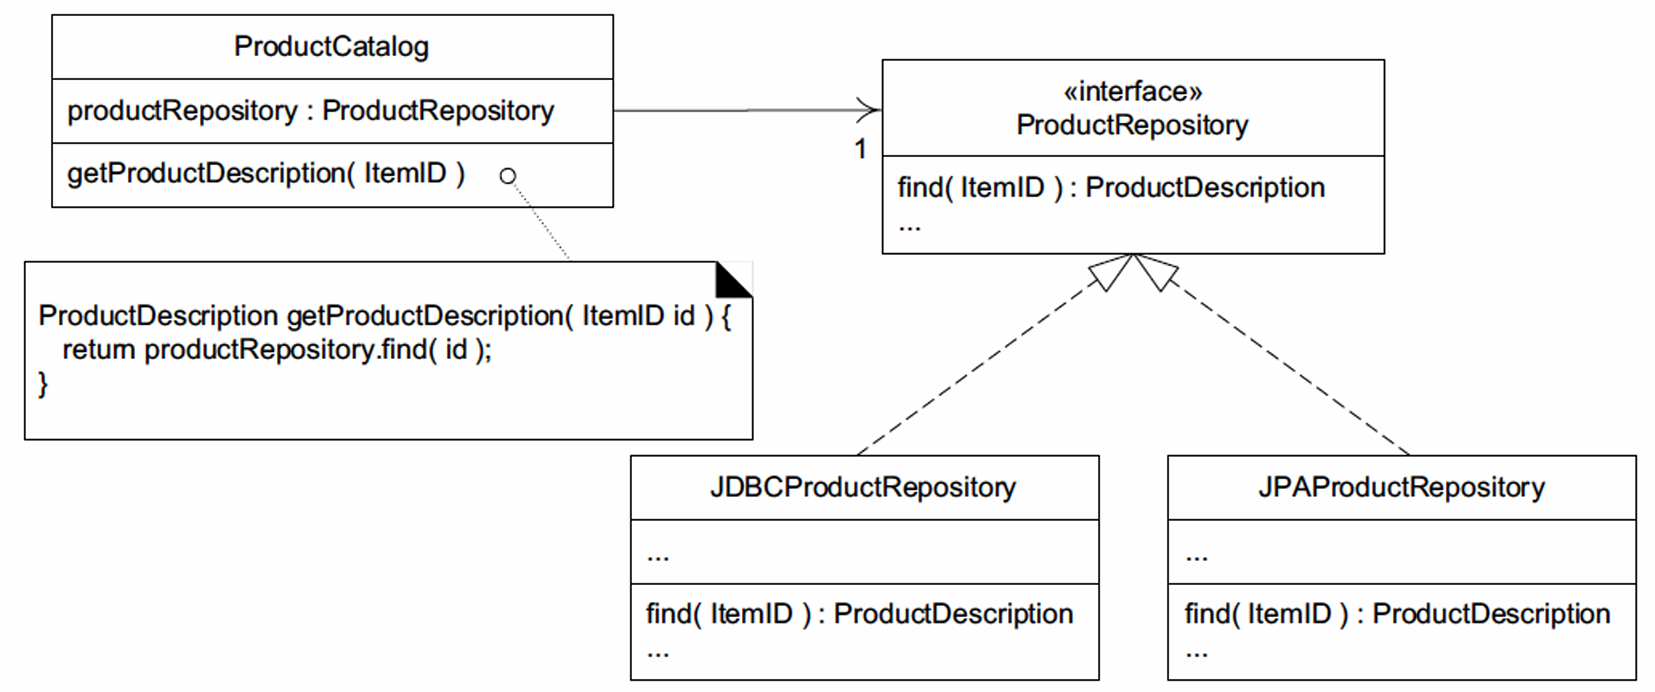
\includegraphics[scale=0.27]{Esercitazione - Design Patterns/repository_pattern.png}
    \end{center}

    In questo esempio abbiamo 3 componenti:
    \begin{enumerate}
        \item \textbf{ProductRepository} è l'interfaccia che funge da repository dei prodotti, viene usata per
        accedere alle informazioni di ciascun prodotto. tramite il metodo \textbf{find()}.
        \item \textbf{JDBCProductRepository} e \textbf{JPAProductRepository} sono delle\\ repository
        contenenti le informazioni.
        \item \textbf{ProductCatalog} è una classe che tramite l'\textit{ItemID} può ottenere la descrizione della
        repository corrispondente.
    \end{enumerate}
    \newpage
}

\mysubsectionformatted{Failover}
\myparagraph{
    Prima di parlare di failover, bisogna definire 3 termini apparentemente uguali:
    \begin{tcolorbox}[colback=green!5!white, colframe=green!75!black]
        \textbf{Fault (Guasto/Difetto):} L'origine o la causa di un comportamento sbagliato
    \end{tcolorbox}

    \begin{tcolorbox}[colback=purple!5!white, colframe=purple!75!black]
        \textbf{Error (Errore):} La manifestazione di un difetto nel sistema
    \end{tcolorbox}

    \begin{tcolorbox}[colback=yellow!5!white, colframe=yellow!75!black]
        \textbf{Failure (Fallimento):} La mancata erogazione di un servizio causata da un errore
    \end{tcolorbox}
    
    \begin{tcolorbox}[colback=blue!5!white, colframe=blue!75!black]
        Per \textbf{Failover} si intende un meccanismo usato per garantire la continuità di un servizio in caso di
        un eventuale guasto o interruzione del sistema. Questo meccanismo agisce in maniera trasparente all'utente,
        simulando le operazioni del sistema principale.
    \end{tcolorbox}
    \vspace{0.1cm}
    \noindent L'obiettivo di un sistema è quello di garantire affidabilità, permettendo il \\ripristino in seguito a guasti esterni.
    La soluzione consiste nel:
    \begin{enumerate}
        \item \textbf{Rendere trasparente la locazione fisica dei dati}
        \item \textbf{Rendere il failover da remoto a locale}
        \item \textbf{Replicare parzialmente i servizi locali}
    \end{enumerate}

    \noindent Nel dettaglio, la soluzione consiste nell'usare un \textbf{Proxy} (fornito da una \\ \textit{ServicesFactory} di tipo Factory)
    in grado di gestire in maniera trasparente e sicura al client eventuali guasti, mascherando la locazione e la disponibilità dei servizi.
    Nel caso in cui un servizio dovesse essere non disponibile, il proxy effettua un failover verso un servizio secondario, senza che il client debba fare nulla.
    \\
    Altro obiettivo del Proxy è far si che realizzi delle implementazioni locali dei servizi remoti che hanno problemi, in modo
    che abbiano un comportamento semplificato e vincolato.
    \\
    Nel pratico, decidiamo di creare una cache locale di oggetti di tipo \\ \textit{ProductDescription}. In questo modo, avremo un aumento
    delle performance e dell'affidabilità.

    \newpage

    \mysubsubsectionformatted{Accesso alla cache locale}

    \begin{wrapfigure}{l}{0.5\textwidth}
        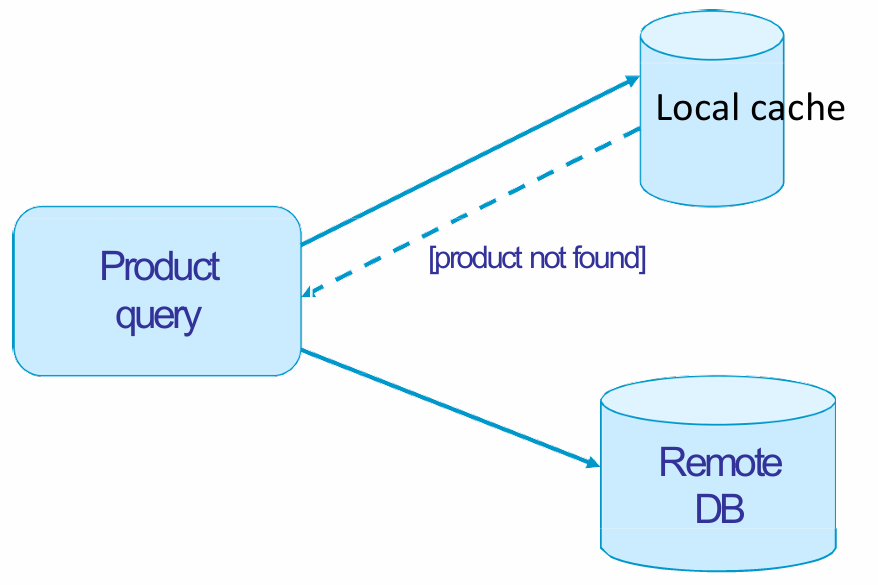
\includegraphics[scale=0.27]{Esercitazione - Design Patterns/Failover - Cache Locale.png}
    \end{wrapfigure}

    \hbadness=2000
    L'accesso alla cache locale avviene tramite il \textit{ServicesFactory}, questo ritorna un adapter a un servizio di 
    informazioni relativo ai prodotti in locale. L'adapter sarebbe l'entità che andrà a implementare le responsabilità del 
    servizio in locale, questo servizio sarà inizializzato con un riferimento verso un secondo adapter, ma quest'ultimo è 
    relativo al corrispondente servizio ma remoto.
    
    In sintesi, nel primo adapter abbiamo le responsabilità del servizio \textbf{locale}, il secondo adapter è relativo al corrispondente servizio
    locale ma in \textbf{remoto}. Se il servizio locale trova il prodotto nella cache (locale), allora lo ritorna, altrimenti inoltra la richiessta all'adapter
    del servizio remoto.
    
    Esistono due tipologie di cache:
    \begin{enumerate}
        \item Cache che mantengono in memoria una collezione di grandezza limitata ma dinamica (es. il \textit{ProductCatalog} che ha in memoria oggetti di tipo \textit{ProductDescription})
        \item Cache che mantengono in memoria una collezione più ampia di elementi su supporti persistenti (es. hard disk), questo implica che, se il sistema dovesse
        malfunzionare, la cache rimane persistente.
    \end{enumerate}

    \noindent \coloredtext[red]{Cosa succede se l'accesso alla cache locale non dà risultato e l'accesso al servizio esterno fallisce?}
    Si verificherà un \textbf{fallimento}, quindi bisogna gestirlo.
    \\
    Una soluzione comune sarebbe quella di \textbf{lanciare un'eccezione}, utile se l'errore si verifica a livello hardware. L'eccezione non deve essere percepita a 
    livello di presentazione (l'utente non deve vedere l'eccezione).
    \\
    Il pattern a cui si fa ricorso è il Design Pattern \coloredtext[blue]{\textbf{Convert Exceptions}} (descritto dopo il pattern Proxy).
    \newpage
}

\mysubsectionformatted{Design Pattern Proxy}
\myparagraph{

\begin{tcolorbox}[colback=blue!5!white, colframe=blue!75!black]
    Il pattern permette l'accesso a quegli oggetti che non sono direttamente\\ accessibili
    o non si desidera fornire l'accesso diretto. Viene creato un oggetto proxy che implementa
    la stessa interfaccia dell'oggetto ed è responsabile del controllo o del miglioramento dell'accesso
    a questo oggetto.
\end{tcolorbox}
\vspace{0.1cm}
    
\begin{center}
    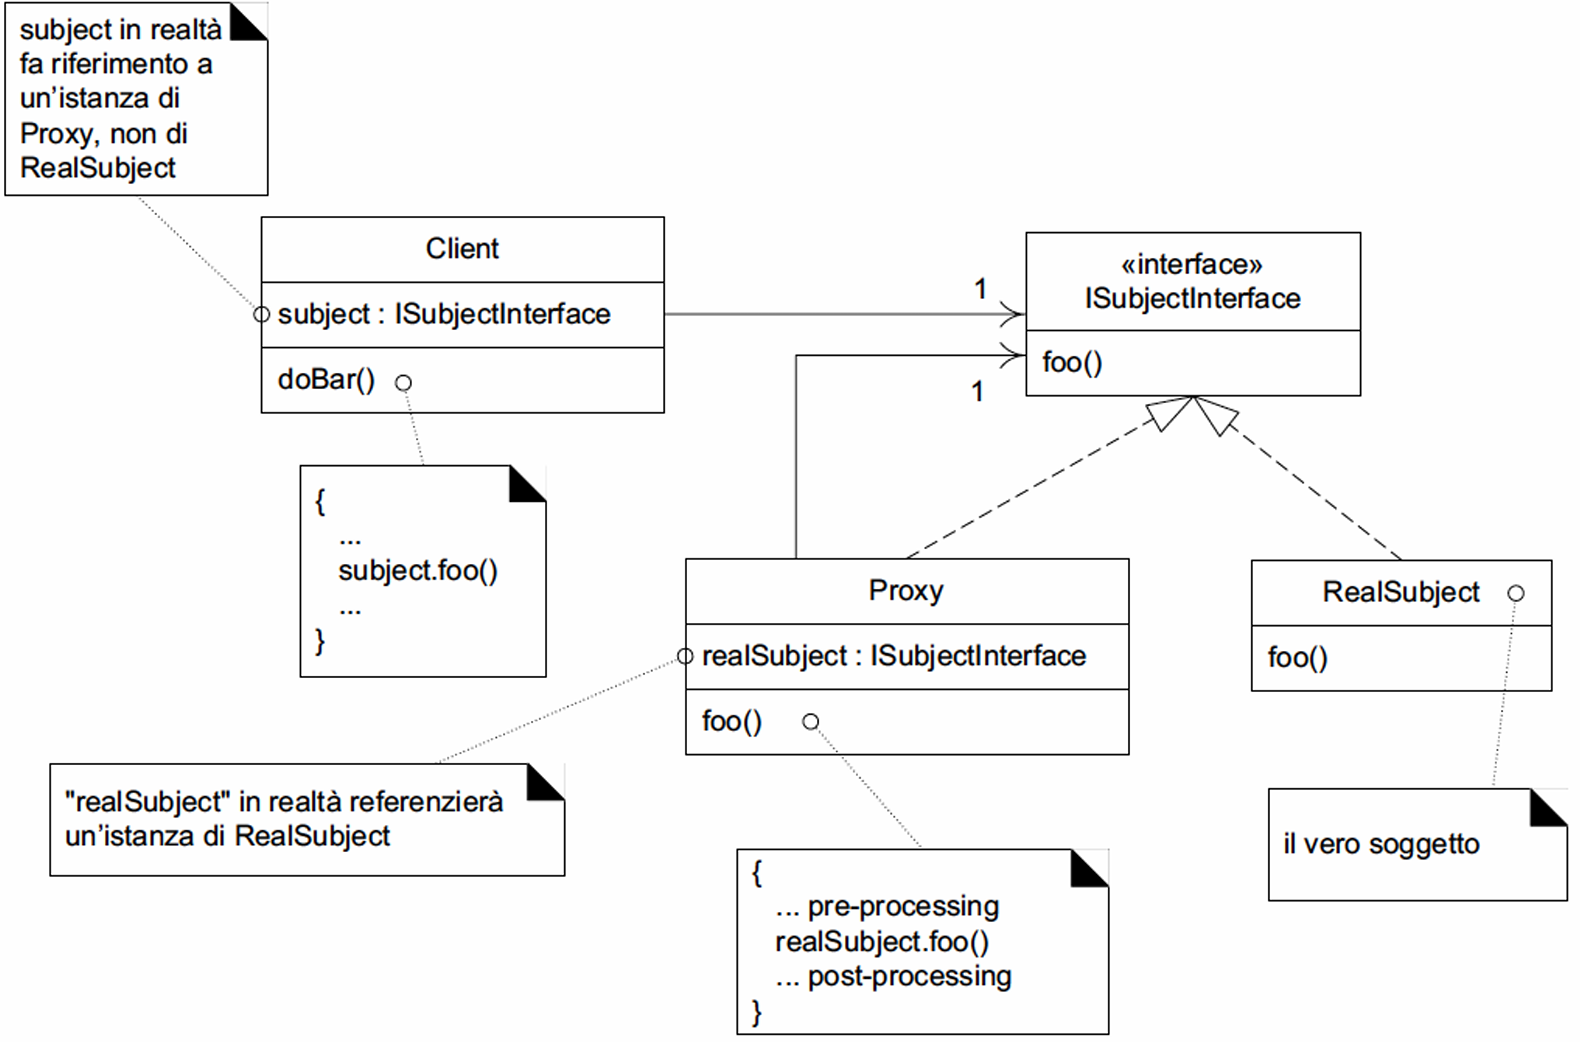
\includegraphics[scale=0.25]{Esercitazione - Design Patterns/proxy_pattern.png}
\end{center}
I componenti del pattern sono:
\begin{enumerate}
    \item \textbf{SubjectInterface} definisce un'interfaccia comune per l'oggetto reale\\ \textbf{RealSubject}
    e il \textbf{Proxy}, permettendo di usarli in modo alternabile.
    \item \textbf{RealSubject} è l'oggetto reale, contiene l'implementazione concreta della logica principale.
    \item \textbf{Proxy} è la classe che implementa la \textbf{SubjectInterface} e controlla l'accesso all'oggetto
    reale, implementando logica extra, contiene un riferimento al \textbf{RealSubject}.
\end{enumerate}
Esistono due strategie di gestione della cache:
\begin{enumerate}
    \item \textbf{Inizializzazione lazy}: la cache viene riempita lentamente man mano che vengono inseriti gli oggetti.
    \item \textbf{Inizializzazione greedy}: la cache viene caricata all'inizio.
\end{enumerate}

\newpage

\mysubsubsectionformatted{Ultime considerazioni sul Proxy}
\begin{enumerate}
    \item Il Proxy è un oggetto esterno che nasconde un oggetto interno.
    \item Il client non sa che sta facendo riferimento al Proxy, ma crede di comunicare direttamente con il sistema interno.
    \item Il Proxy è utile nel caso sia necessaria una ridirezione dei messaggi. 
\end{enumerate}

\newpage
    
}

\mysubsectionformatted{Design Pattern Convert Exceptions}
\myparagraph{
    \begin{tcolorbox}[colback=blue!5!white, colframe=blue!75!black]
        Il pattern permette di convertire un'eccezione di livello basso in un'eccezione più
        significativa a livello del sottosistema dove viene lanciata l'eccezione. L'eccezione
        di livello più alto avvolge quella di livello più basso e aggiunge informazioni per 
        renderla più significativa nel contesto del livello superiore. 
    \end{tcolorbox}

    \noindent Un consiglio è quello di rinominare l'eccezione in base al \textbf{perchè è stata \\lanciata, non come},
    in modo da rendere più semplificare al programmatore capire il problema.
 
    \begin{figure}[htbp]
        \centering
        \begin{minipage}{0.45\textwidth}
            \centering
            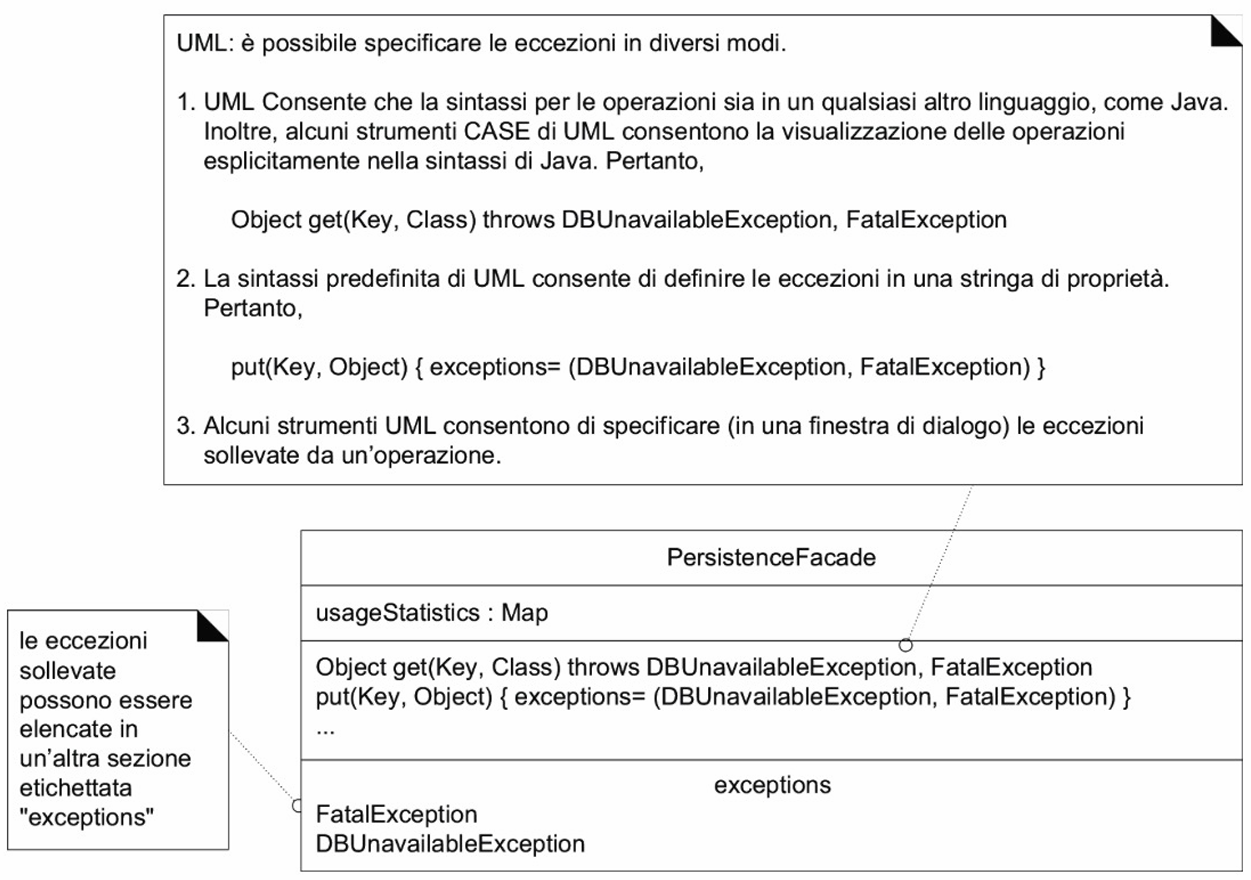
\includegraphics[width=\textwidth]{Esercitazione - Design Patterns/Eccezioni/UML_Eccezioni.png}
            \caption{Eccezioni in un diagramma delle classi}
            \label{fig:immagine1}
        \end{minipage}\hfill
        \begin{minipage}{0.45\textwidth}
            \centering
            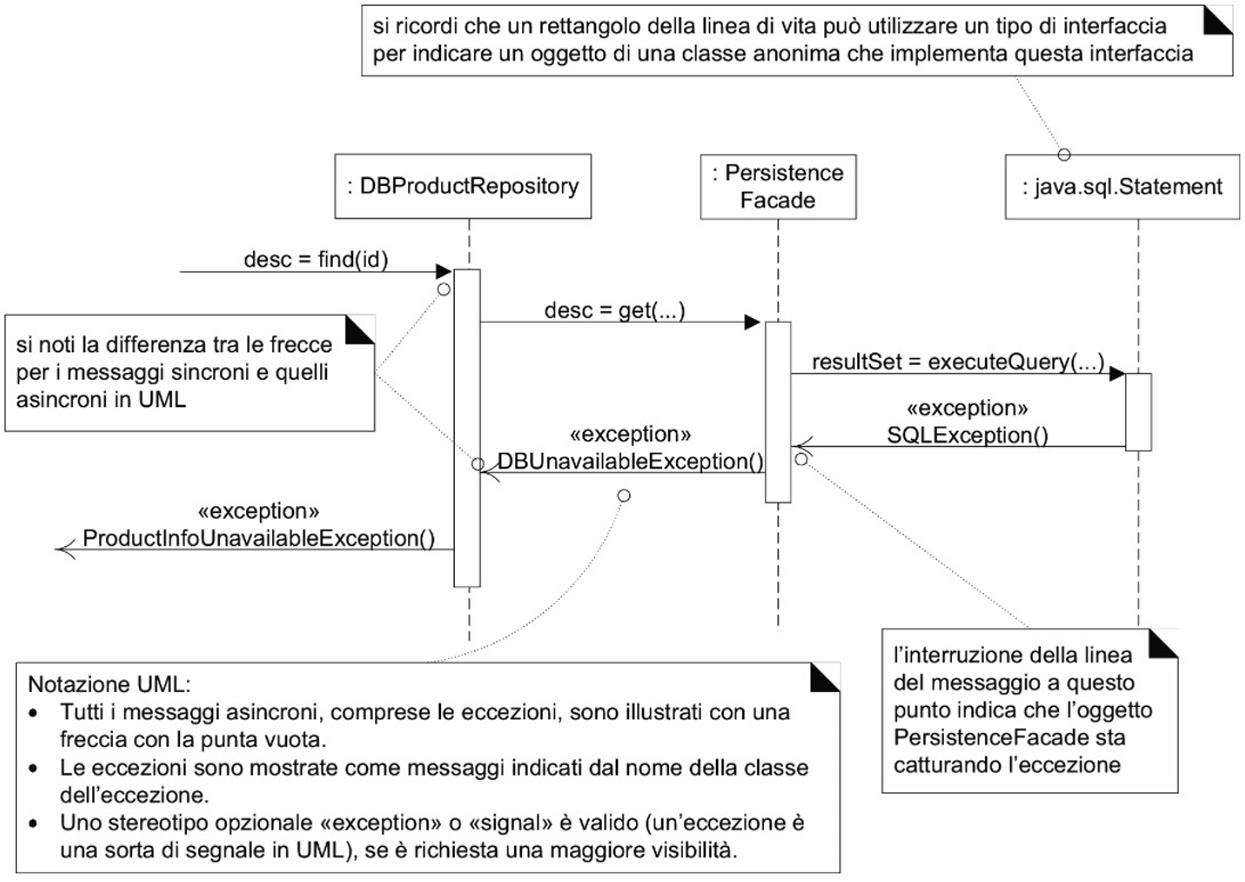
\includegraphics[width=\textwidth]{Esercitazione - Design Patterns/Eccezioni/Diagramma di Sequenza Eccezioni.png}
            \caption{Eccezioni in un diagramma di sequenza}
            \label{fig:immagine2}
        \end{minipage}
    \end{figure}
    \noindent Per gestire l'eccezione, può essere gestita tramite due pattern, il \coloredtext[blue]{\textbf{Centralized Error Logging}} e l'\coloredtext[blue]{\textbf{Error Dialog}}.
    \newpage
    }

\mysubsectionformatted{Design Pattern Centralized Error Logging}
\myparagraph{
    \begin{tcolorbox}[colback=blue!5!white, colframe=blue!75!black]
        Il pattern funge da oggetto centrale per il logging degli errori a cui si
        accede come un Singleton, e si riportano in esso tutte le eccezioni. In caso di
        sistema distribuito, ciascun Singleton locale collaborerà con un logger degli errori centrale.
    \end{tcolorbox}
    \vspace{0.1cm}   
}

\mysubsectionformatted{Design Pattern Error Dialog}
\myparagraph{
    \begin{tcolorbox}[colback=blue!5!white, colframe=blue!75!black]
        Il pattern permette di utilizzare un oggetto non appartenente all'interfaccia utente
        e accessibile attraverso un Singleton con lo scopo di comunicare gli errori agli utenti.
        Il pattern "avvolge" uno o più oggetti della UI (es. una finestra di testo), delegandogli
        la notifica dell'errore. Inoltre, ripoterà l'errore al logger centralizzato degli errori.
        Una \textit{Factory} ha il compito di creare l'oggetto UI appropriato in base ai parametri
        di sistema ricevuti, quindi in base all'errore.
    \end{tcolorbox}
}

\newpage

\mysubsectionformatted{Design Pattern Abstract Factory}
\myparagraph{
    \begin{tcolorbox}[colback=blue!5!white, colframe=blue!75!black]
        Il pattern permette di definire un'interfaccia astratta \textit{Factory} e
        altre classi \textbf{Factory} per ogni famiglia di elementi da creare.
        In questo modo, si possono creare delle famiglie di classi correlate tra loro
        che implementano un'interfaccia comune.
    \end{tcolorbox}

    \setcounter{figure}{0}
    \begin{figure}[h]
        \centering
        \caption{Esempio di Abstract Factory}
        \vspace{0.5cm}
        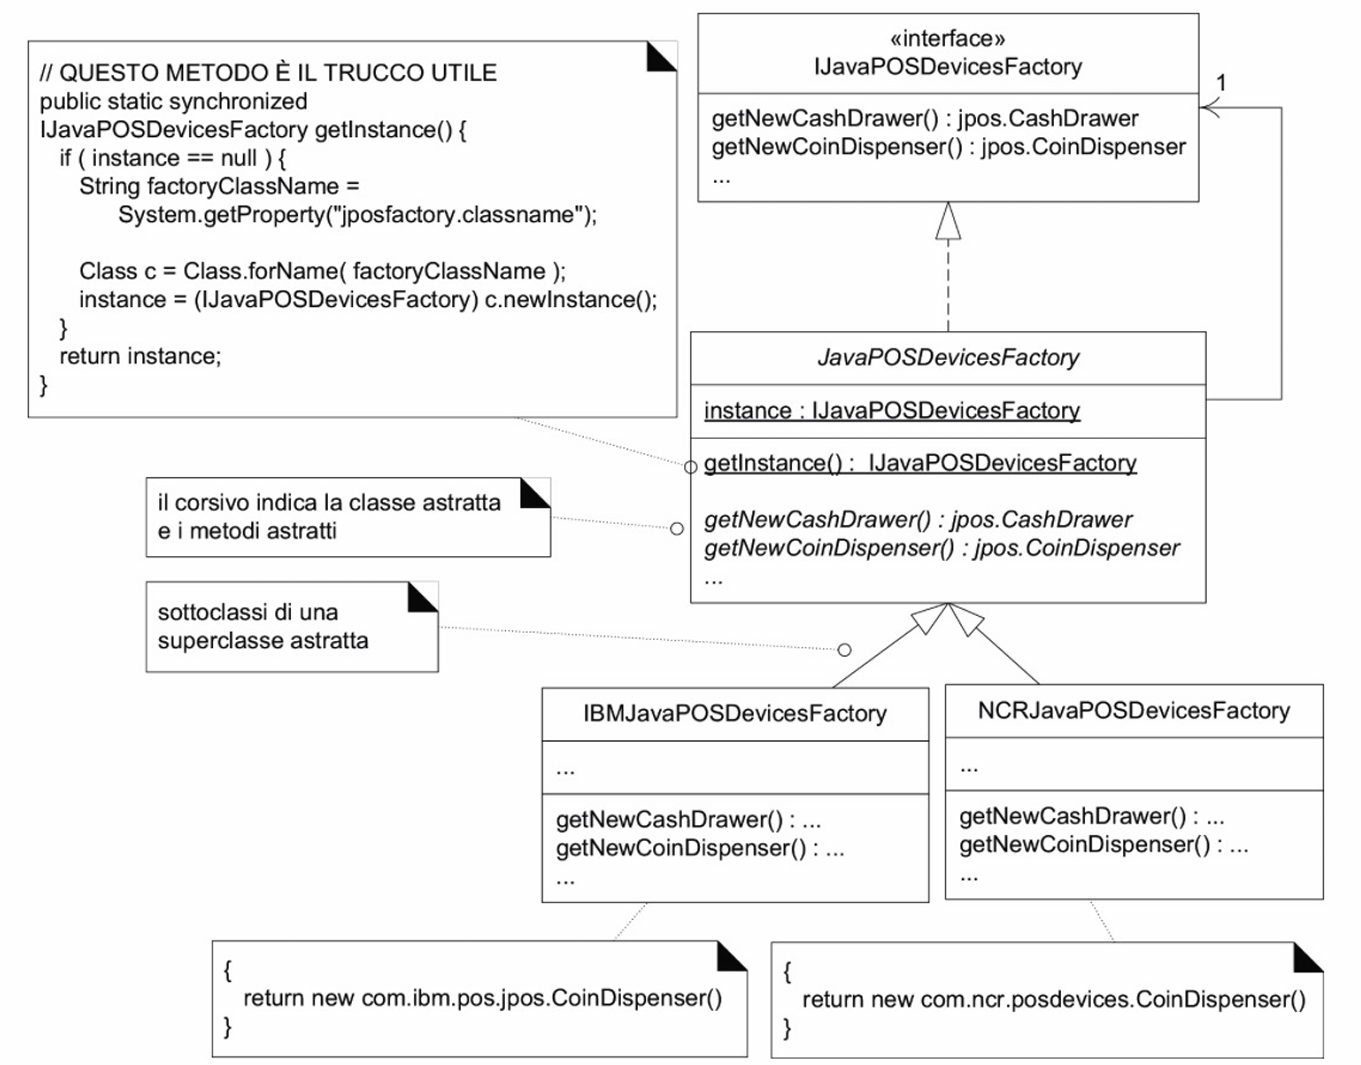
\includegraphics[scale=0.27]{Esercitazione - Design Patterns/Abstract Factory.png}
        \label{fig:pattern}
    \end{figure}

    Spesso, l'\textit{Abstract Factory} viene creata come \textbf{classe astratta}, non come \\interfaccia.\\
    La Factory legge dalle proprietà di sistema quale famiglia di oggetti creare, questo grazie all'aiuto
    del pattern \textbf{Singleton} (con il metodo \textit{getInstance()}).

    \newpage
    }


\mysubsectionformatted{Design Pattern Do It Myself}
\myparagraph{
    \begin{tcolorbox}[colback=blue!5!white, colframe=blue!75!black]
        Chiamato così da Peter Coad, il pattern ha l'obiettivo di applicare il \textbf{Polimorfismo},
        quindi far si che un oggetto software faccia quelle operazioni che normalmente
        verrebbero fatte all'oggetto reale di cui loro sono un'astrazione (loro intesi come gli oggetti software).  
    \end{tcolorbox}

    Detto in modo informale:
    \begin{itemize}
        \item Gli oggetti Quadrato creano se stessi.
        \item Gli oggetti Cerchio creano se stessi.
        \item Gli oggetti Text eseguono il controllo ortografico di se stessi.
    \end{itemize}

    \setcounter{figure}{0}
    \begin{figure}[h]
        \centering
        \caption{Uso del Polimorfismo con i mezzi di pagamento}
        \vspace{0.5cm}
        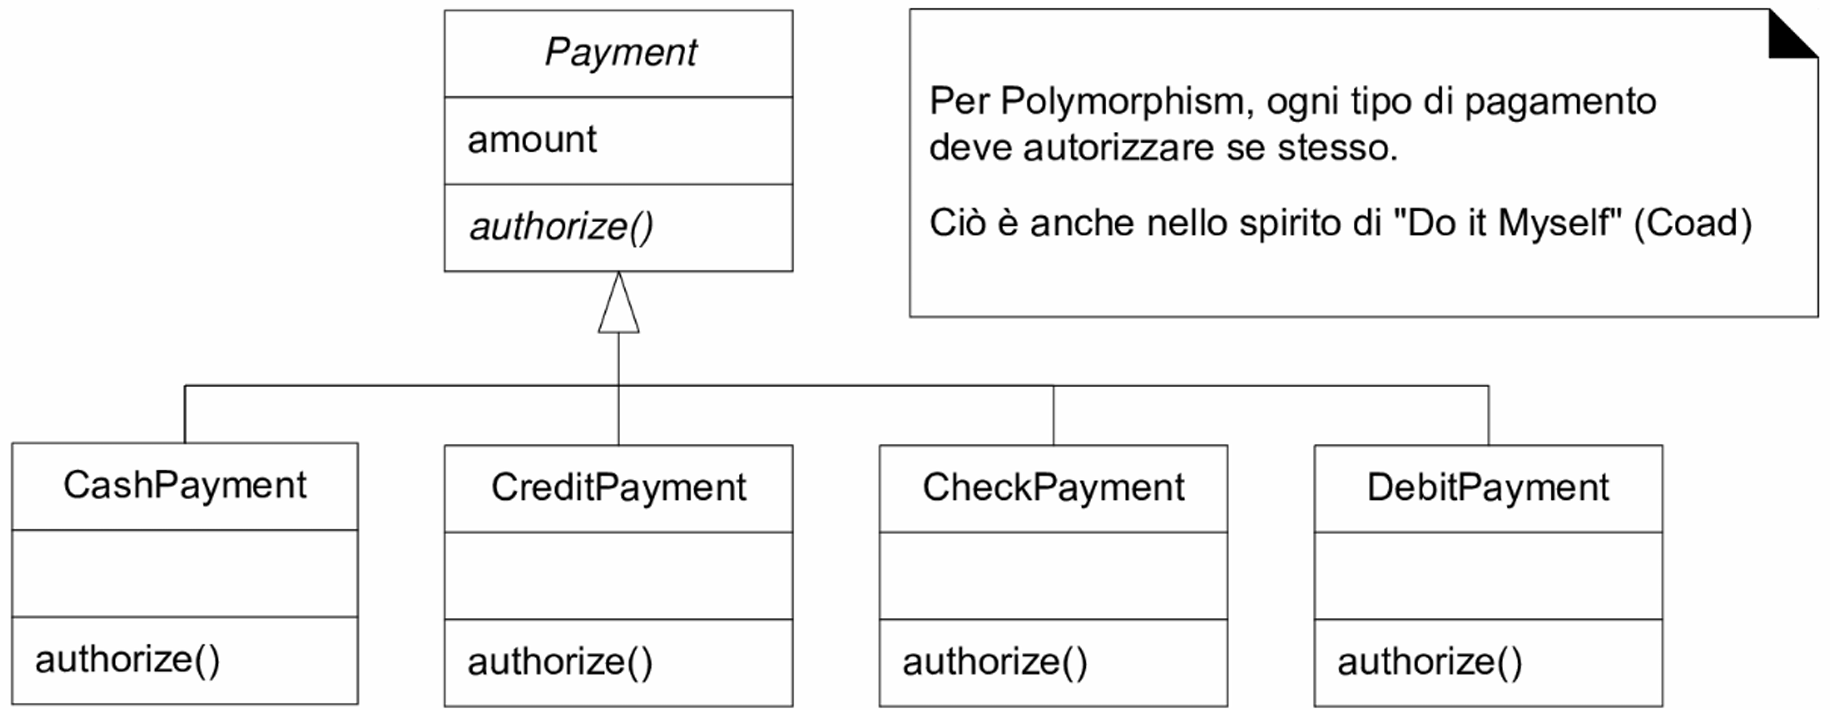
\includegraphics[scale=0.25]{Esercitazione - Design Patterns/Polymorphism.png}
        \label{fig:polymorphism}
    \end{figure}
}
\newpage

\mysubsectionformatted{Progettazione di Framework di persistenza dei dati}
\myparagraph{
    In questa esercitazione, si useranno 4 design pattern già visti per la progettazione
    di framework di persistenza dei dati:
    \begin{enumerate}
        \item Template Method
        \item State
        \item Command
        \item Proxy
    \end{enumerate}
    Quando parliamo di \textbf{Oggetti persistenti}, si intendono quegli oggetti che rimangono
    in memoria durante l'esecuzione del programma, quindi senza che vengano ripristinati alla fine
    dell'esecuzione.

    Solitamente, si fa ricorso ai \textit{database relazionali} che permettono di modellare un
    mapping tra la rappresentazione \textit{record oriented} del database e quella \textit{object-oriented}
    del sistema.

    Ecco alcune definizioni riguardo la persistenza:
    \begin{tcolorbox}[colback=blue!5!white, colframe=blue!75!black]
        Per \textbf{Framework di Persistenza} si intende un insieme di classi e interfacce riusabili, estendibili
        e \textit{general purpose}, che forniscono le funzionalità per la gestione degli oggetti persistenti.
    \end{tcolorbox}

    \begin{tcolorbox}[colback=green!5!white, colframe=green!75!black]
        Per \textbf{Servizio di Persistenza} si intente un sottosistema che fornisce le funzionalità per cooperare
        con il database e generalmente creato dal framework di persistenza.
    \end{tcolorbox}

    \begin{tcolorbox}[colback=red!5!white, colframe=red!75!black]
        Per \textbf{Oggetti Persistenti} si intendono quegli oggetti che necessitano di memorizzazione persistente.
    \end{tcolorbox}

    \mysubsubsectionformatted{Proprietà dei framework}
    \hbadness=10000
    \begin{enumerate}
        \item \`E un insieme coeso di interfacce e classi che collaborano tra loro per fornire servizi per la parte
        fondamentale e invariabile di un sottosistema logico.
        \item Contiene classi concrete e astratte che definiscono le interfacce a cui conformarsi e le interazioni tra
        gli oggetti.
        \item Di solito, richiede all'utente di definire delle sottoclassi di classi esistenti del framework per personalizzare
        ed estendere i servizi del framework.
        \item Ha delle classi astratte che possono contenere metodi astratti e concreti.
    \end{enumerate}

    \mysubsubsectionformatted{Servizio di persistenza}
    Un compito fondamentale del \textbf{Servizio di Persistenza} è quello di \textbf{effettuare il mapping fra
        la rappresentazione a oggetti e rappresentazione relazionale dei dati}, per farlo, compie due operazioni:
    \begin{enumerate}
        \item \textbf{Materializzazione}: traduzione di record in oggetti (caricamento in memoria).
        \item \textbf{Dematerializzazione}: traduzione di oggetti in record (memorizzazione nel DB).
    \end{enumerate}

    Per creare un servizio di persistenza, si deve realizzare un framework di persistenza che abbia le seguenti funzionalità:
    \begin{enumerate}
        \item Memorizzazione e recupero degli oggetti in e da un sistema di storage persistente.
        \item Fornire transazioni coerenti di \textbf{commit} e \textbf{rollback}.
        \item Deve essere estendibile per poter supportare diversi meccanismi e formati di memorizzazione (es. XML).
    \end{enumerate}

    I \textbf{punti chiave} per progettare un framework di persistenza sono:
    \begin{enumerate}
        \item Mapping.
        \item Indetificazione univoca degli oggetti.
        \item Materializzazione e Dematerializzazione degli oggetti (mediante pattern \textit{Template}).
        \item Gestione dello stato degli oggetti persistenti (mediante pattern \textit{State}).
        \item Modellazione delle operazioni relative a una transazione quali commit e rollback (mediante pattern \textit{Command}).
        \item Lazy materialization (mediante pattern \textit{Proxy}).
        \item Aumento delle performance con l'uso della cache.
    \end{enumerate}

    \newpage
    \mysubsubsectionformatted{Mapping}
    Il mapping risponde alla domanda \textit{"Come facciamo a far corrispondere un oggetto a un record in un DB relazionale?"}

    \subsubsection{Design Pattern Representing Objects as Tables}
    Un pattern utile allo scopo è il \coloredtext[blue]{\textbf{Representing Objects as Tables}}.
    \myparagraph{
    \begin{tcolorbox}[colback=blue!5!white, colframe=blue!75!black]
        Il pattern permette di definire una tabella per ciascuna classe di oggetti persistenti
        dentro un DB relazionale. Gli attributi degli oggetti corrisponderanno alle colonne della tabella e
        conterranno oggetti di tipo primitivo.
    \end{tcolorbox}
}

    \mysubsubsectionformatted{Identificazione univoca di oggetti}
    Questo punto chiave permette di non ripetere la materializzazione di oggetti molteplici volte, col rischio di creare oggetti
    duplicati.

    \subsubsection{Design Pattern Object Identifier}
    Il pattern utile allo scopo è l'\coloredtext[blue]{\textbf{Object Identifier}}.
    \myparagraph{
    \begin{tcolorbox}[colback=blue!5!white, colframe=blue!75!black]
        Il pattern permette di assegnare a ogni record di tabella e a ogni oggetto un
        valore alfanumerico chiamato Object ID che consente l'immediata identificazione
        di ogni istanza.
    \end{tcolorbox}

    \begin{center}
        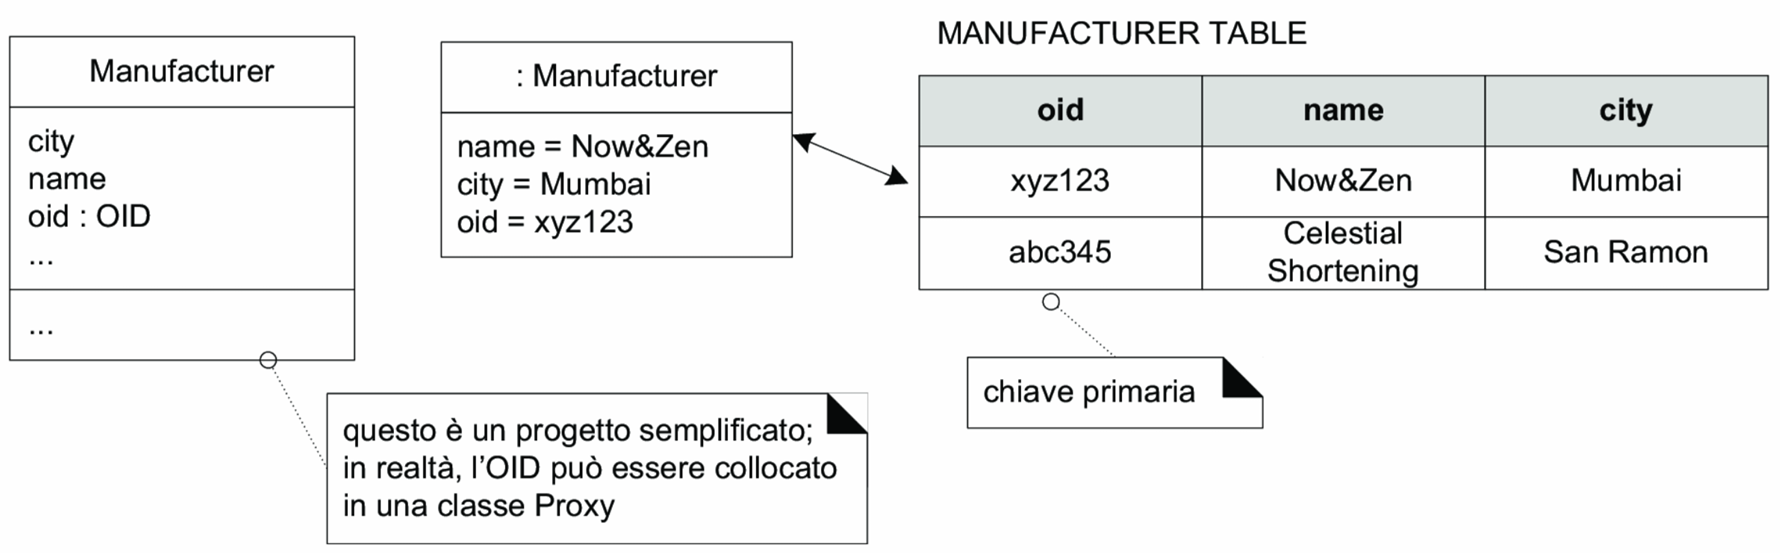
\includegraphics[scale=0.25]{Esercitazione - Design Patterns/Object Identifier.png}
    \end{center}
}

    \newpage
    \mysubsubsectionformatted{Accesso a un Servizio di Persistenza}
    Un pattern utile a fornire un unico punto di accesso è il \textbf{Facade}.
    \subsubsection{Design Pattern Facade}
    \myparagraph{
    \begin{tcolorbox}[colback=blue!5!white, colframe=blue!75!black]
        Il pattern fornisce un'interfaccia unificata ai servizi forniti di un certo sottosistema.
        La Facade delega le richieste provenienti dai client verso gli oggetti del sottosistema che nasconde. 
        Il suo intento è quello di rendere più semplice l'uso di un sottosistema.
    \end{tcolorbox}

    \vspace{0.1cm}
    \begin{center}
        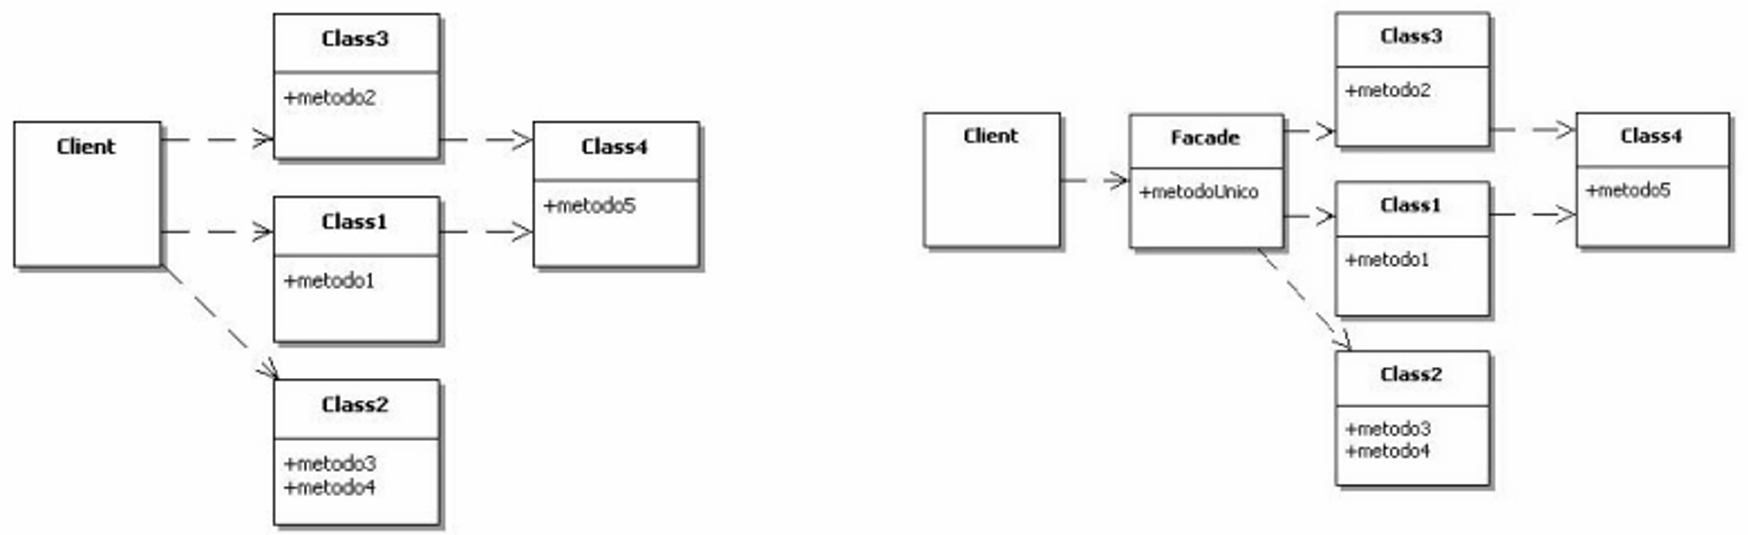
\includegraphics[scale=0.25]{Esercitazione - Design Patterns/Facade.png}
    \end{center}
    I partecipanti del pattern sono:
    \begin{enumerate}
        \item \textbf{Facade}: Conosce le classi responsabili per una richiesta e delega le richieste dei client
        agli oggetti appropriati del sottosistema.
        \item \textbf{Classi del sottosistema}: Implementano le funzionalità del sottosistema e gestiscono il lavoro
        assegnato dal Facade, questo però senza aver alcun riferimento di quest'ultima.
    \end{enumerate}

    Bisogna fare alcune considerazioni riguardo questo pattern:
    \begin{enumerate}
        \item Diminuisce l'accoppiamento tra client e sottosistema.
        \item Nasconde al client le componenti del sottosistema.
        \item Il client può comunque usare direttamente le classi del sottosistema.
    \end{enumerate}
    Si può anche rendere il Facade una classe astratta con sottoclassi concrete per diminuire ulteriormente
    l'accoppiamento. I client possono comunicare con il sottosistema mediante l'interfaccia della classe astratta Facade.

    \mysubsubsectionformatted{Facade vs Adapter}
    \begin{enumerate}
        \item Entrambi sono dei wrapper.
        \item Entrambi si basano su un'interfaccia, però:
        \item \begin{enumerate}
            \item Facade lo semplifica.
            \item Adapter lo converte.
        \end{enumerate}
    \end{enumerate}
}

    \mysubsubsectionformatted{Materializzazione e Dematerializzazione}
    In questa sezione vedremo \textbf{chi si occupa della Materializzazione e \\l'archiviazione degli oggetti}.

    Esistono due tipi di \textbf{Mapping}:
    \begin{enumerate}
        \item \textbf{Direct Mapping}: una classe che rappresenta un oggetto persistente \\definisce al suo interno il codice
              per il suo salvataggio nel DB (il codice è generato in automatico).
        \item \textbf{Indirect Mapping}: esistono classi apposite volte al recupero e al salvataggio dei dati in un DB.
    \end{enumerate}

    Questi due tipi di mappature si possono rappresentare mediante due pattern: \coloredtext[blue]{\textbf{Active Record}} per il Direct e \coloredtext[blue]{\textbf{Database Mapper}}
    per l'Indirect.

    \newpage
    \mysubsectionformatted{Active Record - Direct Mapping}
\myparagraph{
    \begin{tcolorbox}[colback=blue!5!white, colframe=blue!75!black]
        Il pattern architetturale permette di convertire ciascuna classe di dominio in tabella del DB.
        Combina i dati e il comportamento di un'entità in un'unica classe e inserisce la
        logica di accesso ai dati nell'oggetto di dominio, in modo che tutti sappiano come leggere e
        scrivere i dati da/al DB.
    \end{tcolorbox}
    
    \begin{center}
        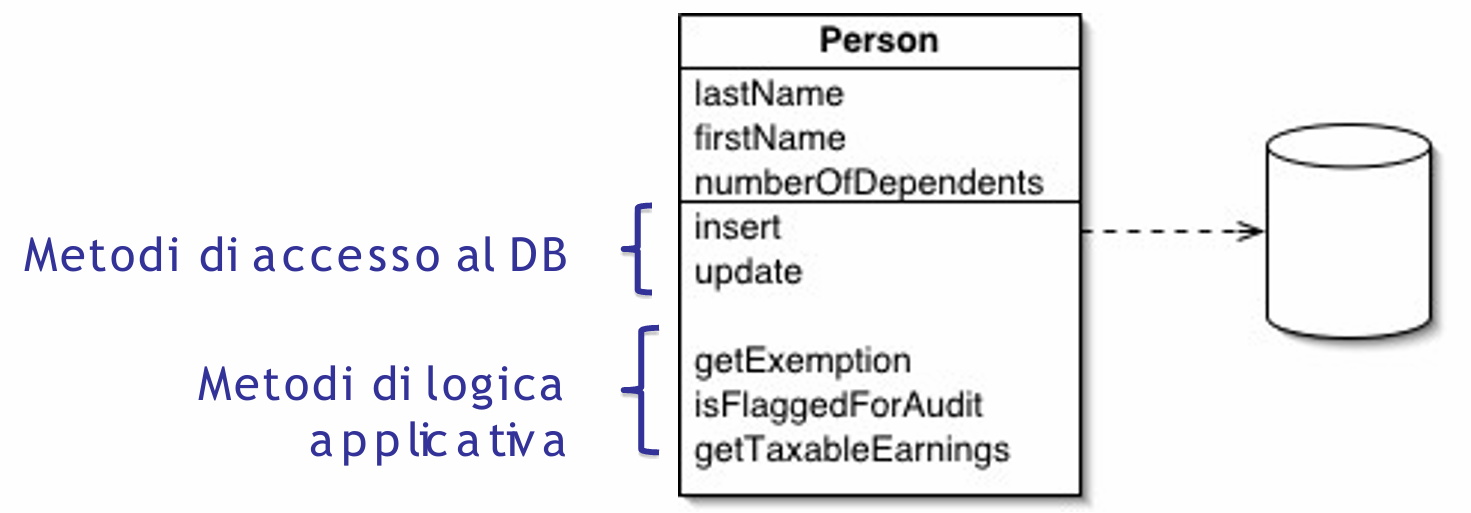
\includegraphics[scale=0.25]{Esercitazione - Design Patterns/Active Record.png}
    \end{center}

    Active Record fa uso di alcuni metodi e strutture dati:
    \begin{enumerate}
        \renewcommand{\labelenumii}{\arabic{enumi}.\arabic{enumii}}
        \item \textbf{Metodo load}: costruisce un'istanza partendo dai risultati generati da una query SQL.
        \item \textbf{Metodi finder} statici: incapsulano le query SQL e ritornano le istanze degli oggetti.
        \item \textbf{Costruttore classico}: costruisce nuove istanze da inserire successivamente nel DB.
        \item \textbf{Metodi di aggiornamento del DB}:
              \begin{enumerate}
                  \item \textbf{update}: aggiorna un record esistente con i valori degli attributi.
                  \item \textbf{insert}: aggiunge un record utilizzando i valori degli attributi.
                  \item \textbf{delete}: elimina il record corrispondente dell'oggetto corrente.
              \end{enumerate}
        \item \textbf{Metodi accessors}:
              \begin{enumerate}
                  \item I metodi \textbf{set} e \textbf{get} per accede ai campi.
                  \item Effettuano la conversione dei dati per memorizzare i valori degli attributi in un formato SQL-oriented.
                  \item Possono richiedere un'immediata sincronizzazione del DB.
              \end{enumerate}
        \item \textbf{Metodo di logica di business}
    \end{enumerate}
    \vspace{0.1cm}

    \resizebox{\columnwidth}{!}{%
        \begin{tabular}{l|l|}
            \hline
            \rowcolor[HTML]{32CB00}
            \multicolumn{1}{|c|}{\cellcolor[HTML]{32CB00}\textbf{Vantaggi}} & \multicolumn{1}{c|}{\cellcolor[HTML]{FE0000}\textbf{Svantaggi}}                                                                                     \\ \hline
            \multicolumn{1}{|l|}{Semplice da implementare e usare}          & \begin{tabular}[c]{@{}l@{}}L'accoppiamento fra la logica applicativa e il DB\\ rende difficile il refactoring dei due progetti\end{tabular}         \\ \hline
                                                                            & \begin{tabular}[c]{@{}l@{}}Si cerca di mantenere una corrispondenza stretta (o quasi)\\ fra lo schema del DB e l'entità del modello OO\end{tabular} \\ \cline{2-2}
        \end{tabular}%
    }
}
    \newpage
    \mysubsectionformatted{Database Mapper - Indirect Mapping}
\myparagraph{
    \begin{tcolorbox}[colback=blue!5!white, colframe=blue!75!black]
        Il framework (o pattern di progettazione) permette di definire una classe che si occupi della gestione dei processi
        di materializzazione da un DB, la dematerializzazione della memoria verso il DB e
        il caching degli oggetti con l'obiettivo di aumentare la performance del sistema.
    \end{tcolorbox}

    Il pattern definisce un DB Mapper per ogni classe di oggetti persistenti, possono esistere diversi
    tipi di Mapper a seconda dei meccanismi di memorizzazione.

    \begin{center}
        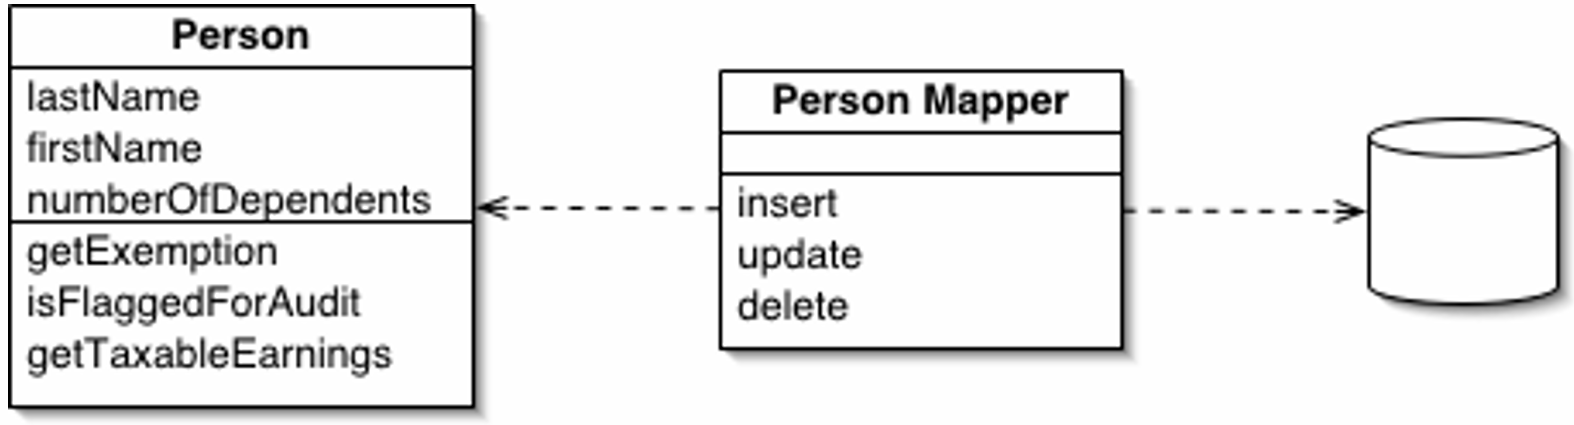
\includegraphics[scale=0.25]{Esercitazione - Design Patterns/Database Mapper.png}
    \end{center}

    \textbf{Person Mapper} è uno strato separato di componenti dedicati a trasferire i dati fra l'applicazione
    (\textbf{Person}) e il \textbf{Database}, trattando indipendentemente i due schemi (OO e ER). Infatti, la
    logica di business è inconsapevole dell'esistenza del Database.\\
    Generalmente, il pattern ne coinvolge di ulteriori per la gestione della sincronizzazione fra i due schemi
    (es. \textit{UnitOfWork} o \textit{IdentityMap}).\\
    Usiamo questo pattern per \textbf{gestire un mapping complesso fra DB e logica di business}.

    \begin{center}
        \resizebox{\columnwidth}{!}{%
            \begin{tabular}{ll}
                \hline
                \rowcolor[HTML]{32CB00}
                \multicolumn{1}{|c|}{\cellcolor[HTML]{32CB00}\textbf{Vantaggi}} & \multicolumn{1}{c|}{\cellcolor[HTML]{FE0000}\textbf{Svantaggi}} \\ \hline
                \multicolumn{1}{|l|}{Isola totalmente i due strati}             & \multicolumn{1}{l|}{Difficolta nell'implementazione}            \\ \hline
                                                                                &
            \end{tabular}%
        }
    \end{center}
    \newpage
}

    \mysubsectionformatted{Materializzazione in cache}
    Vogliamo mantenere all'interno della cache locale gli oggetti che sono stati materializzati in modo da:
    \begin{enumerate}
        \item Aumentare le prestazioni
        \item Supportare la gestione delle transazioni
    \end{enumerate}

    Il pattern utile allo scopo è il \coloredtext[blue]{\textbf{Cache Management}}
    \mysubsubsectionformatted{Design Pattern Cache Management}
    \myparagraph{
    \begin{tcolorbox}[colback=blue!5!white, colframe=blue!75!black]
        Il pattern estende il design pattern \textbf{Database Mapper}, facendo si che siano
        responsabili per la gestione della cache. Ogni Mapper può mantenere e gestire una propria
        cache privata. Il pattern verifica prima di tutto se gli oggetti sono in cache
        prima di recuperarli dal DB per evitare materializzazioni inutili.
    \end{tcolorbox}
}
    L'algoritmo di materializzazione, in pseudocodice, è strutturato in questo modo:
    \vspace{-0.1cm}
    \begin{algorithm}
        \caption{Gestione Cache}
        \begin{algorithmic}[1]
            \If{l'oggetto è in cache}
            \State ritorna l'oggetto
            \Else
            \State materializza l'oggetto dal database
            \State salva l'oggetto in cache
            \State ritorna l'oggetto
            \EndIf
        \end{algorithmic}
    \end{algorithm}
    \vspace{-0.1cm}

    Per progettare questa funzionalità, il pattern utile allo scopo è il \textbf{Template Method} (visto nella prima esercitazione).
    Il template method sarà il metodo \textbf{get} in una superclasse astratta. Ogni mapper specifico darà poi la sua implementazione
    di come ottenere i propri oggetti dal repository.

    \setcounter{figure}{0}
    \begin{figure}[H]
        \caption{Template Method per la materializzazione}
        \centering
        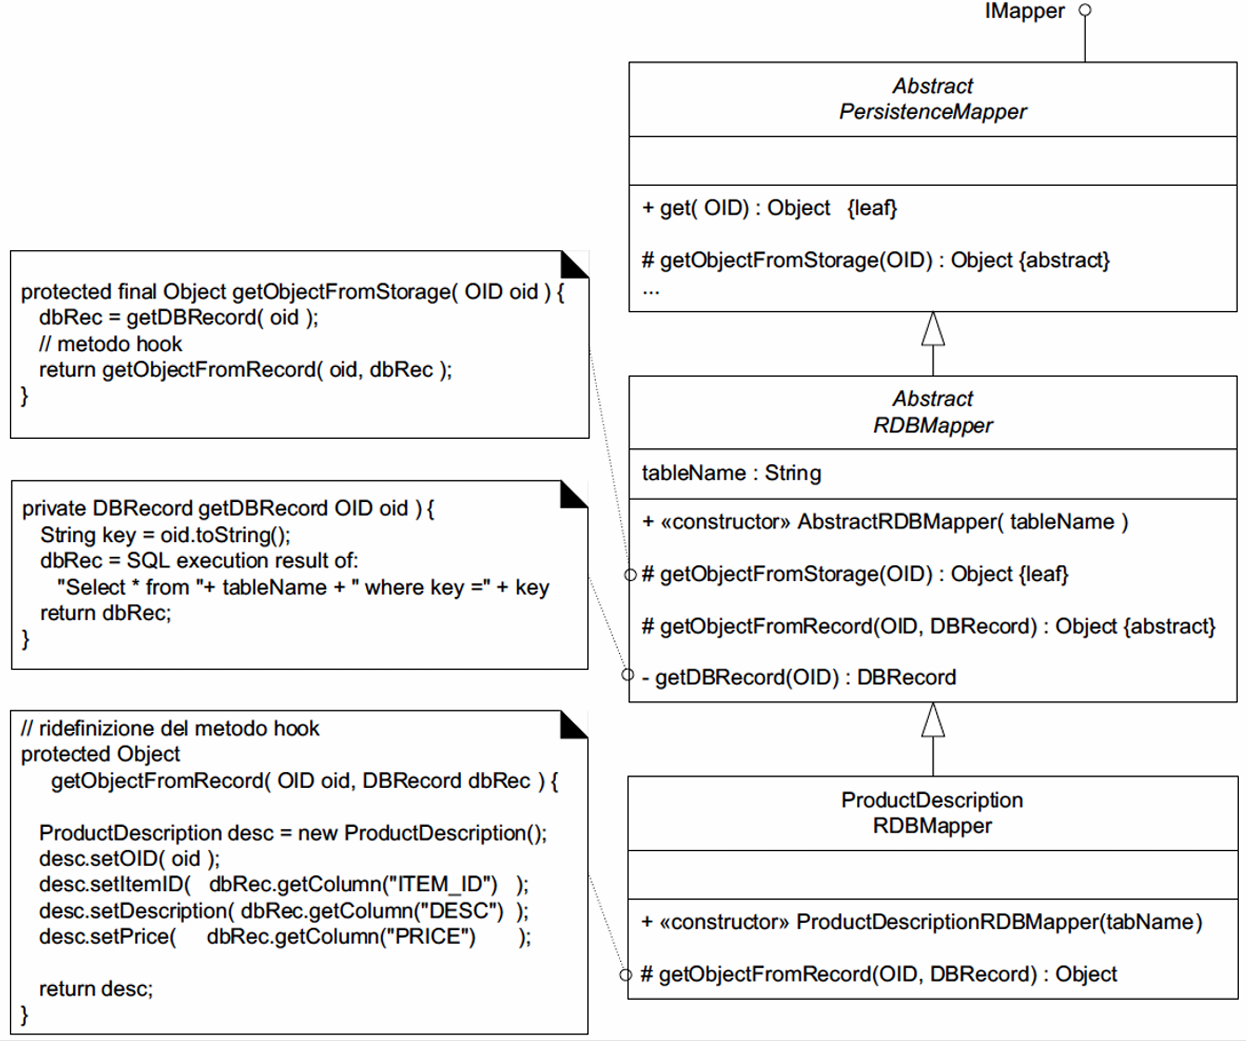
\includegraphics[scale=0.18]{Esercitazione - Design Patterns/Template Method Materializzazione.png}
    \end{figure}

    \newpage
    Fino ad'ora, le query SQL sono sempre state inserite dentro al codice dei metodi.

    \begin{center}
        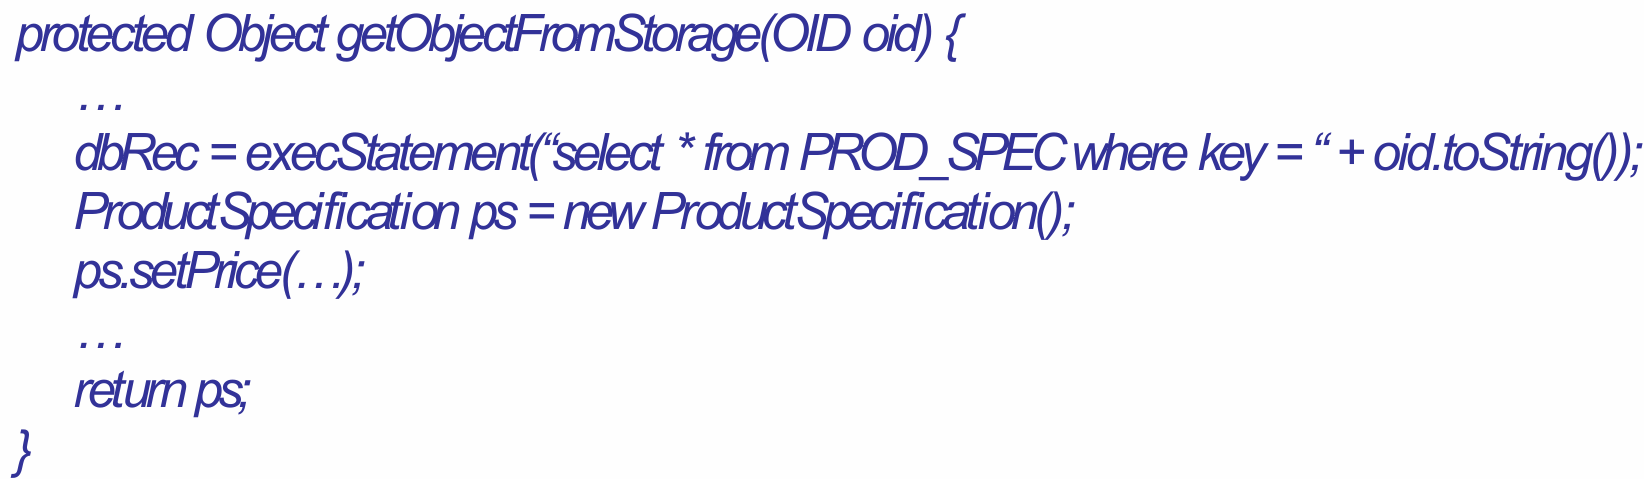
\includegraphics[scale=0.25]{Esercitazione - Design Patterns/Template Method SQL/Fase 1.png}
    \end{center}

    Per migliorare l'implementazione,
    si può mantenere una classe \textbf{Singleton} dove memorizzare tutte le query SQL necessarie (RDBOperations).

    \begin{center}
        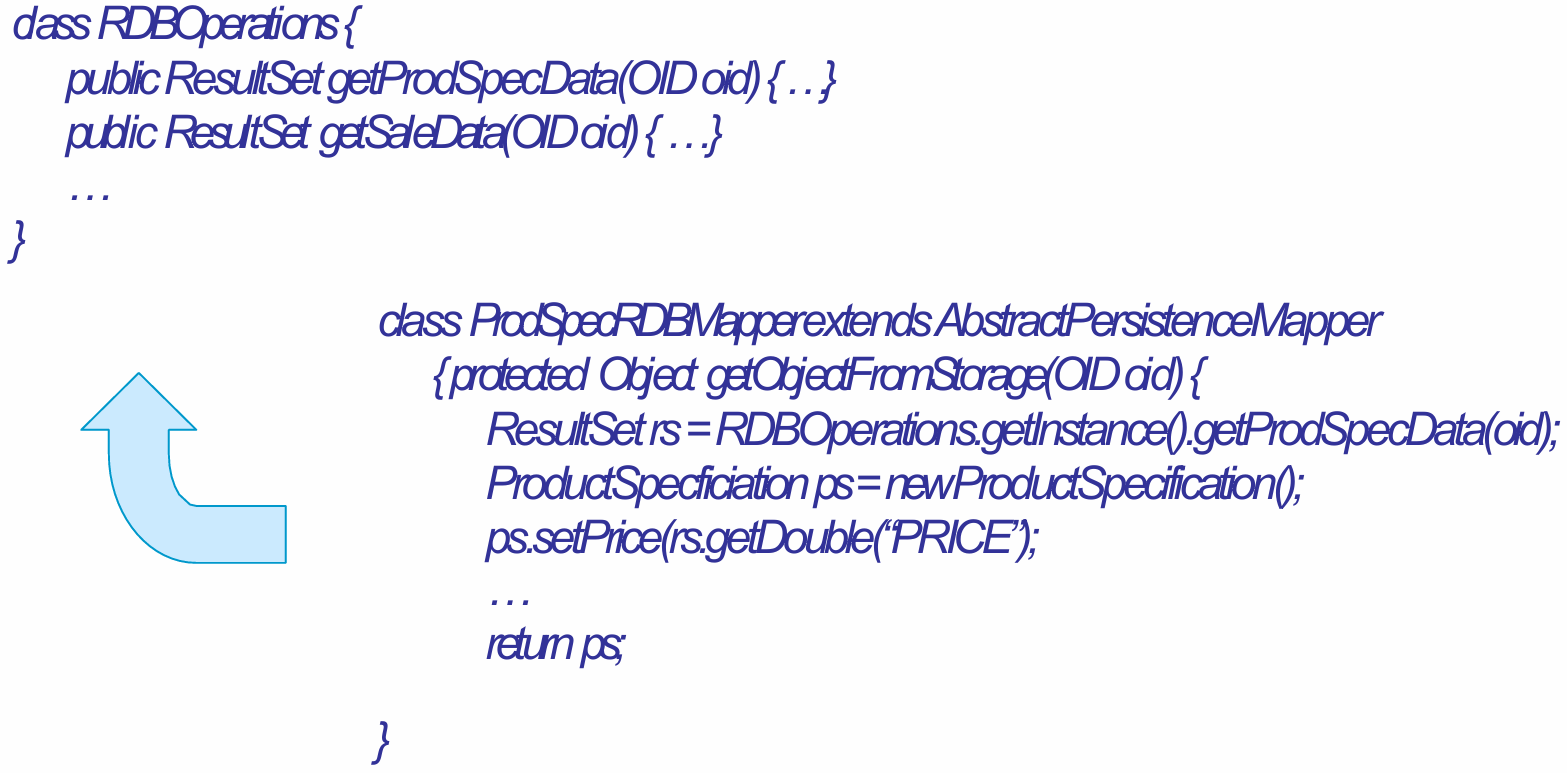
\includegraphics[scale=0.25]{Esercitazione - Design Patterns/Template Method SQL/Fase 2.png}
    \end{center}

    Risulta vantaggioso isolare le query in modo da rendere più facile la manutenzione migliorare la performance.
    \newpage
    }

\mysubsectionformatted{Transazioni e Stati transazionali}
\myparagraph{
    Una \textbf{Transazione} è un'unità di lavoro i cui compiti devono essere completati tutti con successo,
    oppure nessuno di essi deve essere completato. 

    Quando lavoriamo su oggetti persistenti (li inseriamo, cancelliamo o aggiorniamo), questi non vengono aggiornati
    subito nel database, bisogna quindi eseguire un'operazione di commit esplicita.
    Possiamo definire \textbf{3 luoghi} in cui possono trovarsi gli oggetti persistenti:
    \begin{enumerate}
        \item nell'applicazione
        \item nel database
        \item nella cache
    \end{enumerate} 

    Si possono anche definire gli \textbf{stati} associati agli oggetti persistenti:
    \begin{enumerate}
        \item \textbf{New}: appena creato e non ancora presente nel DB
        \item \textbf{Old}: recuperato dal DB (quindi creato in precedenza) 
        \item \textbf{Clean}: non modificato
        \item \textbf{Dirty}: modificato
        \item \textbf{Deleted}: cancellato
    \end{enumerate}

    \setcounter{figure}{0}

    \begin{figure}[h]
        \caption{Diagramma degli Stati}
        \centering
        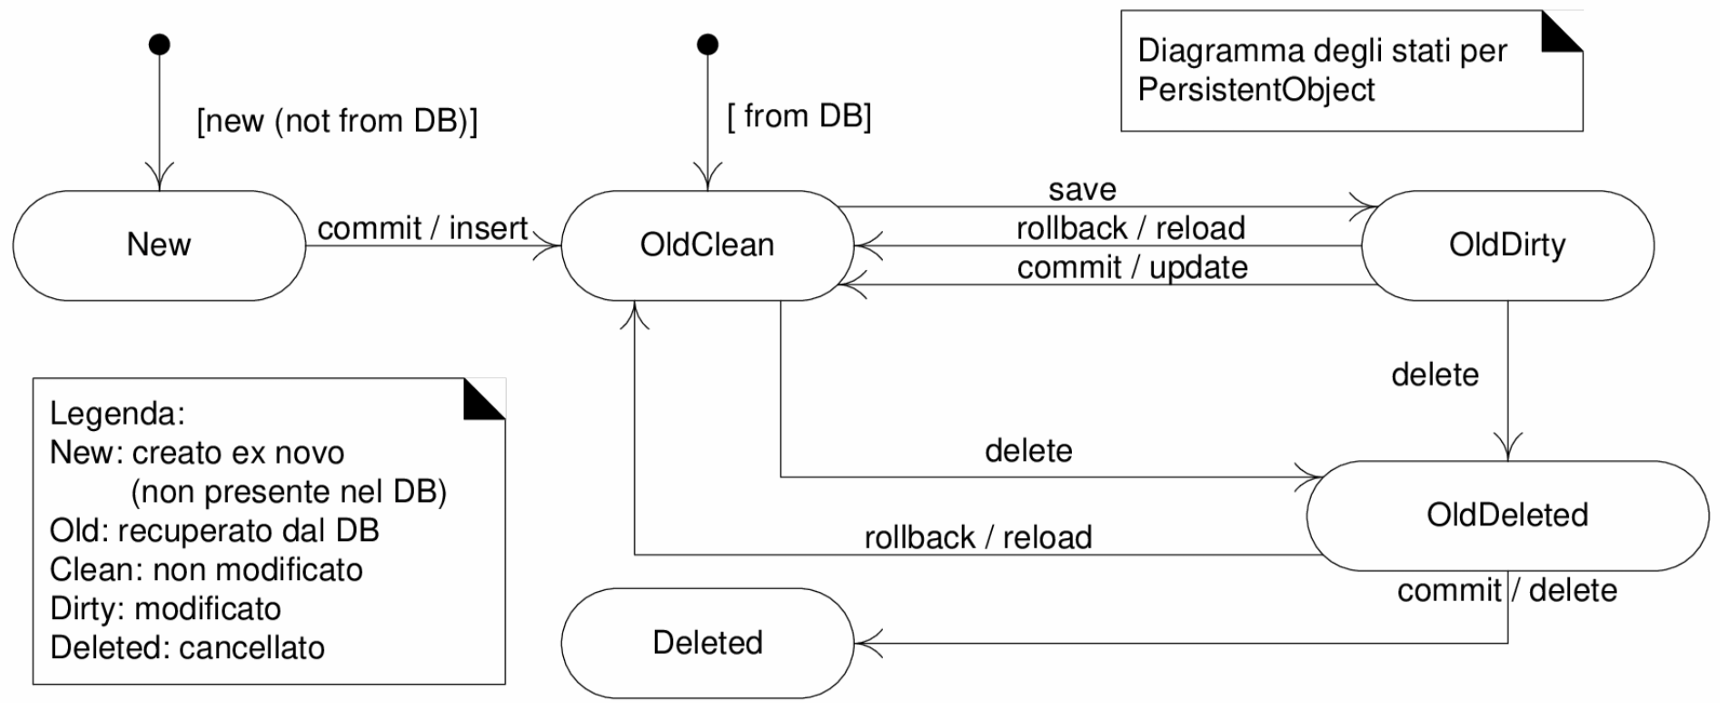
\includegraphics[scale=0.27]{Esercitazione - Design Patterns/Diagramma degli Stati.png}
    \end{figure}
    \textbf{Nota:} quando salviamo o cancelliamo un oggetto persistente, questo non viene immediatamente
    salvato/cancellato dal DB, ma vanno in uno stato appropriato (OldDirty o OldDeleted) in attesa di un eventuale rollback
    (annullo l'operazione) o commit (procedo con l'operazione).
    \newpage
    Il comportamento di \textbf{commit} e \textbf{rollback} sono molto simili tra loro (in termini di codice)

    \begin{center}
        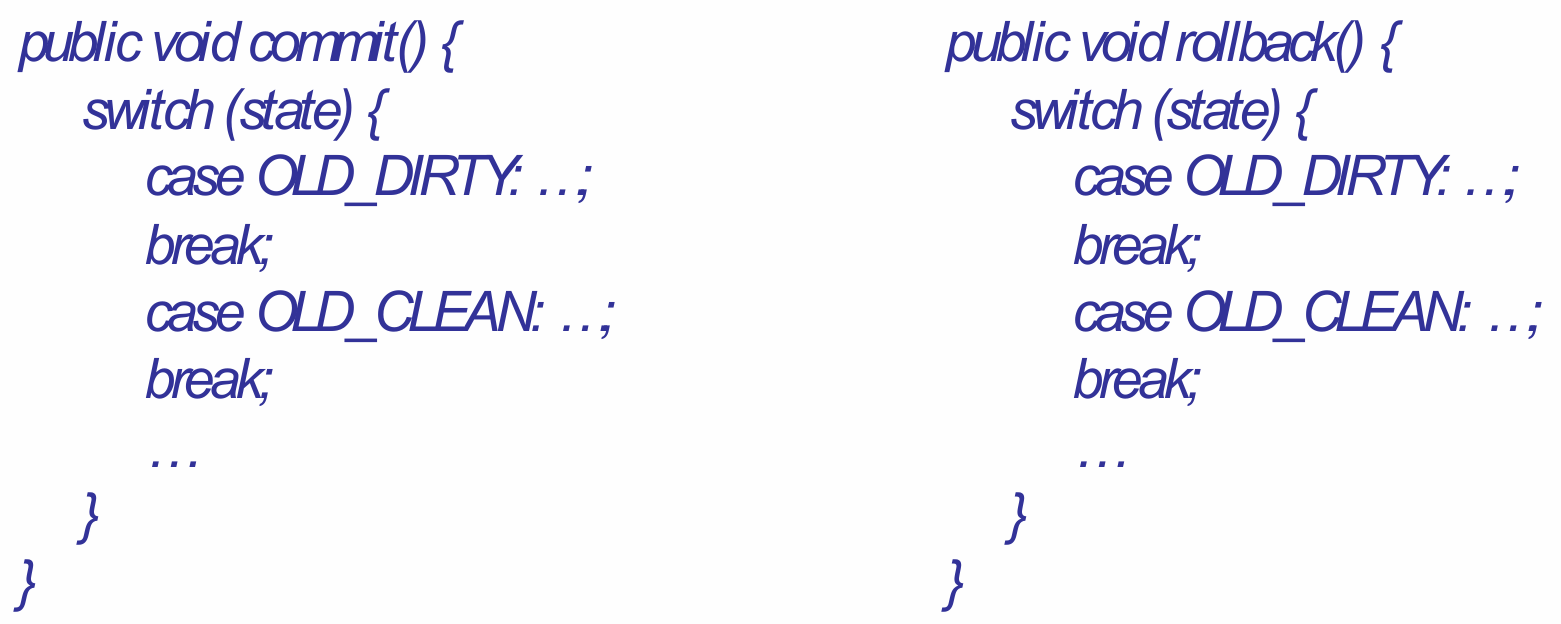
\includegraphics[scale=0.25]{Esercitazione - Design Patterns/Commit e Rollback.png}
    \end{center}
    Per evitare una ripetizione di codice, usiamo il pattern \textbf{State}:
    \begin{center}
        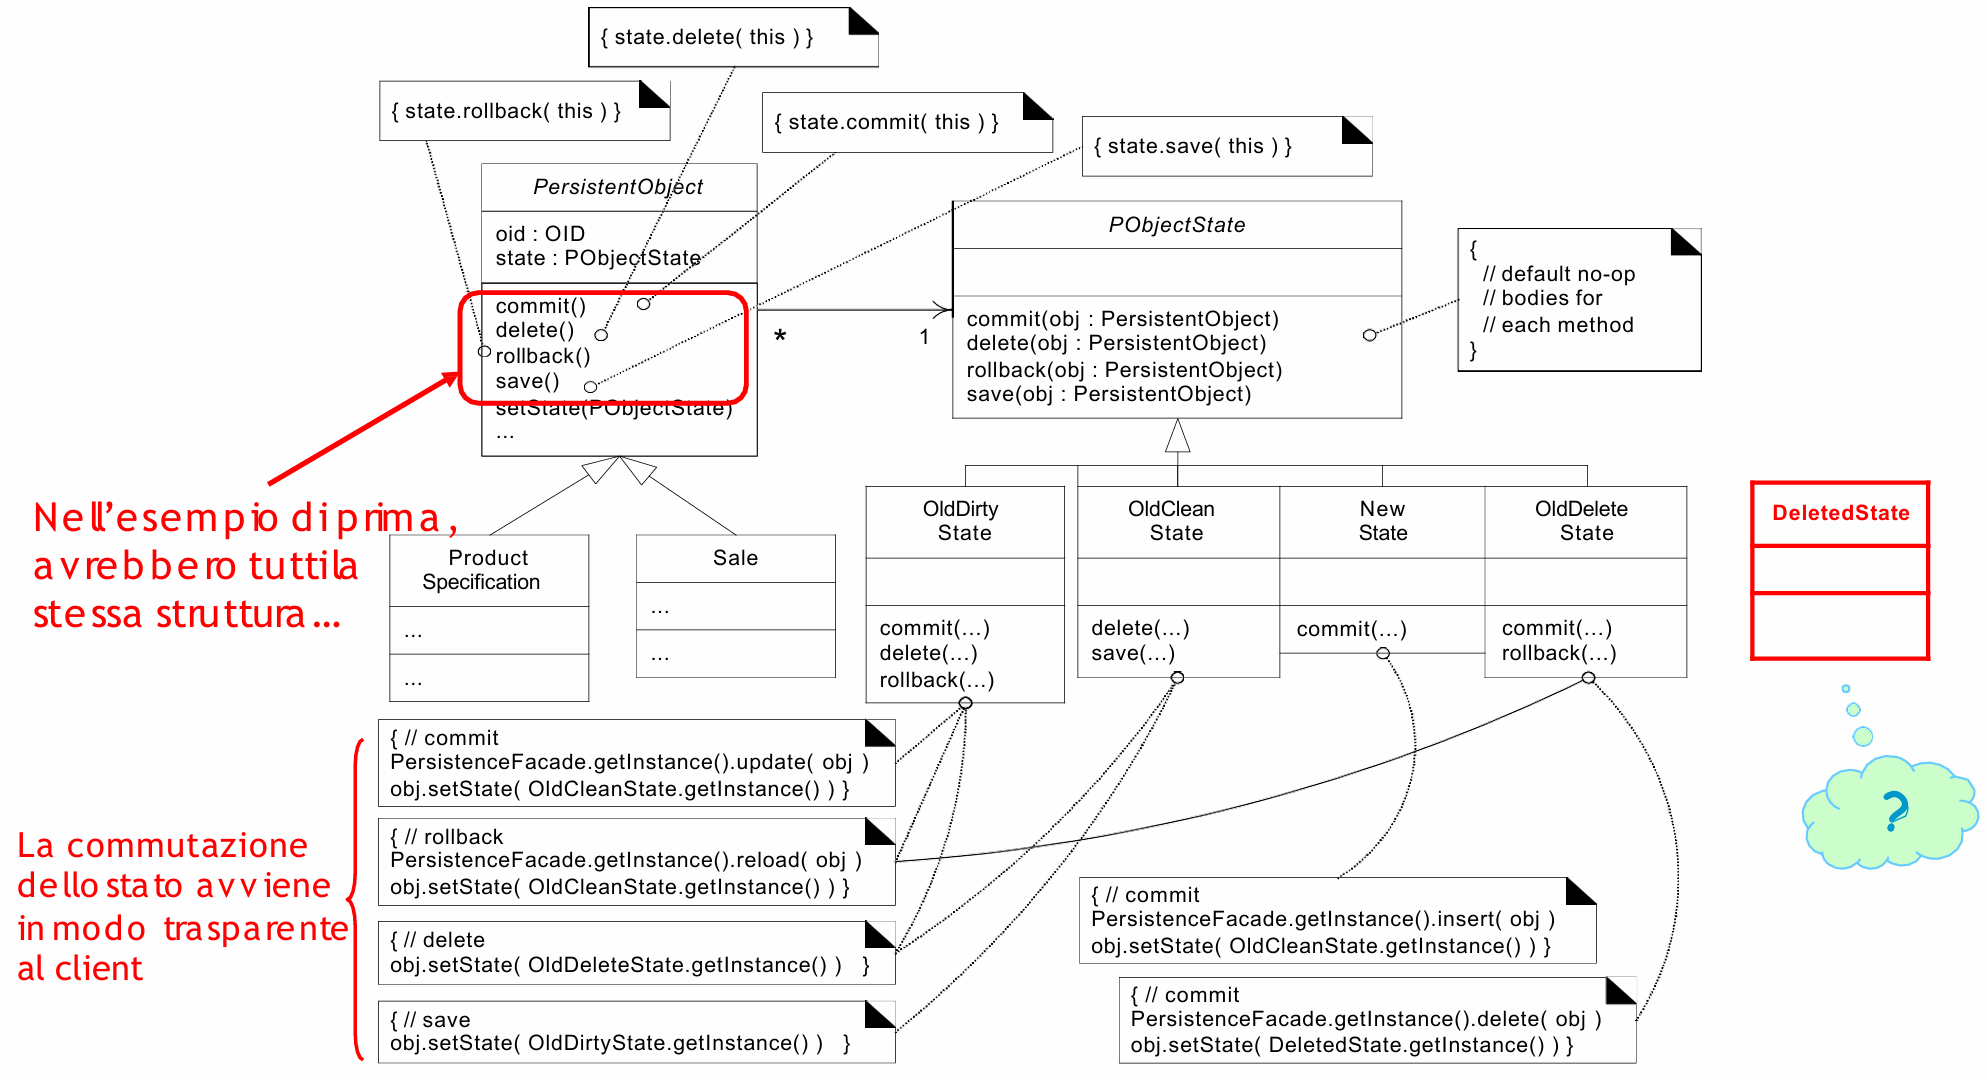
\includegraphics[scale=0.24]{Esercitazione - Design Patterns/State con Commit e Rollback.png}
    \end{center}
    Ricordando cosa fa lo State, crea delle classi che indicano gli stati, le classi implementano un'interfaccia
    comune. Questa interfaccia delega le operazioni all'oggetto \textbf{contesto} in base al suo stato corrente.

    Nell'esempio sopra il \textit{PersistentObject} rappresenta l'oggetto \textbf{Context}, mentre \textit{PObjectState}
    l'interfaccia \textbf{\textit{State}}. Per ogni stato concreto, definiamo le operazioni appropriate.
    \newpage
    \mysubsubsectionformatted{Modellazione delle operazioni di una transazione}
    Le transazioni, ovviamente, possono essere molteplici. In base all'ordine in cui vengono eseguite le operazioni all'interno
    di una transazione, si può influenzare la performance della transazione. Bisogna quindi trovare una soluzione, ovvero un modo
    per poter riordinare tutte le operazioni uguali prima di essere eseguiti. In questo ambito, interviene il pattern \textbf{Command}.
    
    Ricordando cosa fa Command, definisce per ciascun compito una classe che implementa un'interfaccia comune, a differenza di State che
    rappresentava uno stato, \textbf{nel Command ciascuna classe rappresenta un comando} e le azioni diventano oggetti.
    \begin{center}
        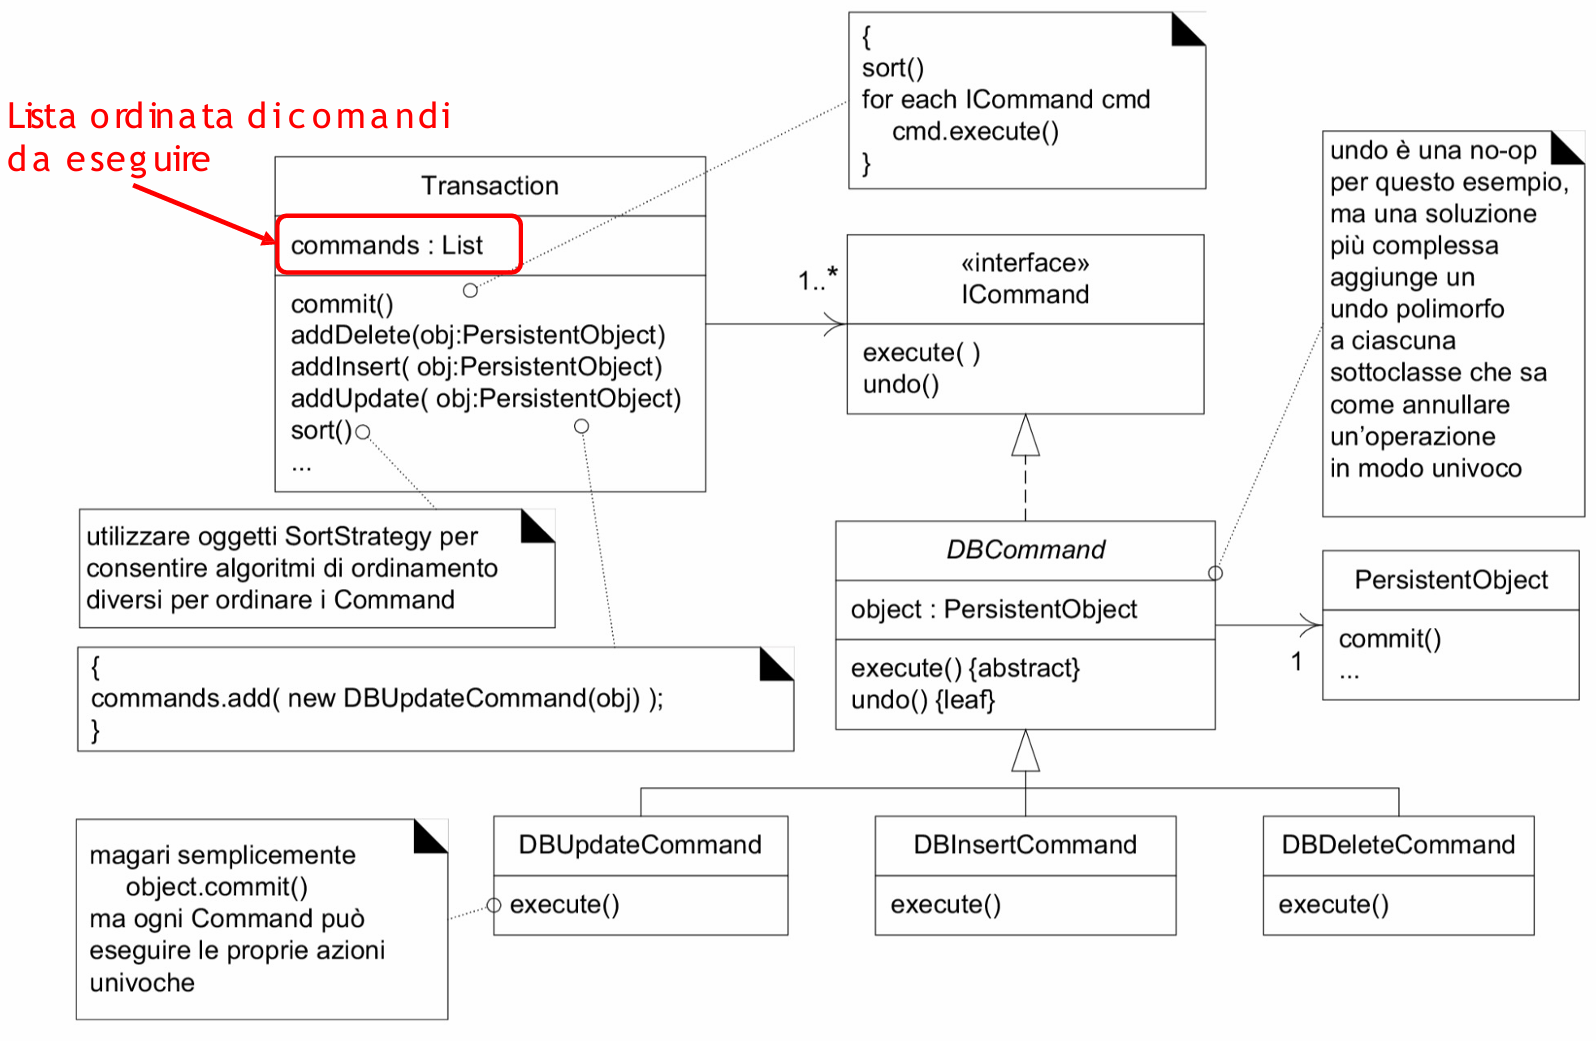
\includegraphics[scale=0.24]{Esercitazione - Design Patterns/Command con Commit e Rollback.png}
    \end{center}
    Nell'esempio, la classe Transaction è l'\textbf{invoker}, ovvero la classe che richiede all'interfaccia \textit{\textbf{ICommand}} le
    operazioni da eseguire. L'interfaccia riceve le operazioni e la classe DBCommand (la \textbf{ConcreteCommand}) incapsula le operazioni, per
    poi farle eseguire dal \textbf{Receiver}, ovvero la PersistentObject.
    \newpage
    \mysubsubsectionformatted{Lazy materialization con l'uso di Proxy}
    Ricordando la definizione di materializzazione, si tratta della traduzione di un record di un DB a un oggetto.

    A volte si vuole evitare il processo di materializzazione, per questioni di performance e a meno che non sia strettamente necessario. Si può
    risolvere questo problema tramite un processo di materializzazione "ritardata", ovvero la \textit{Lazy Materialization}.

    Il pattern utile allo scopo è il \coloredtext[blue]{\textbf{Virtual Proxy}}.
    \mysubsubsectionformatted{Design Pattern Virtual Proxy}
    \myparagraph{
    \begin{tcolorbox}[colback=blue!5!white, colframe=blue!75!black]
        Il Virtual Proxy è un Proxy per l'oggetto "reale", questo proxy virtuale
        materializza l'oggetto solo la prima volta a cui gli si fa riferimento,
        rappresentandoli come oggetti leggeri che fungono da sostituto all'oggetto
        reale (che possono essere più pesanti).
    \end{tcolorbox}

    In sostanza, il Virtual Proxy funge da sostituto dell'oggetto reale, ma in un formato
    più leggero. Sarà questo sostituto a gestire l'accesso all'oggetto reale e a caricarlo
    in memoria solo quando è strettamente necessario, in modo da evitare materializzazioni
    inutili.

    \begin{wrapfigure}{r}{0.55\textwidth}
        \begin{center}
          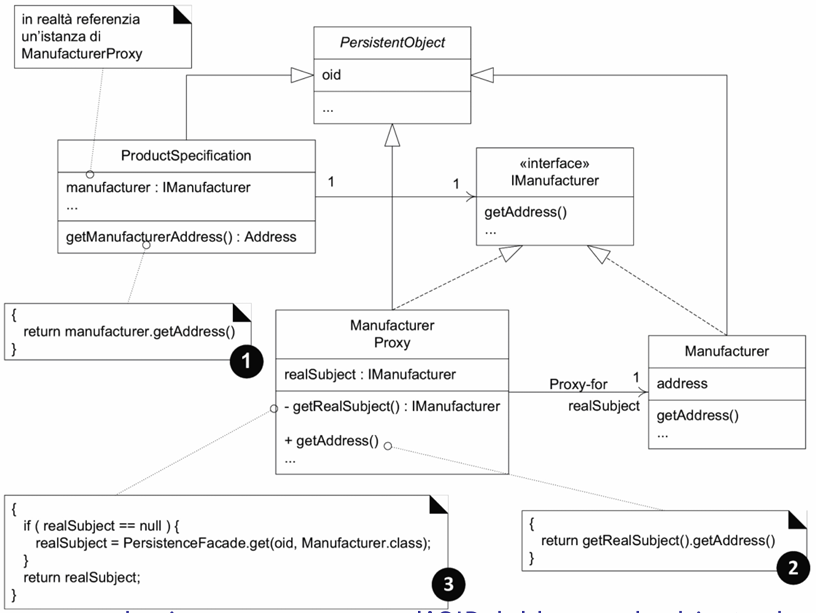
\includegraphics[width=0.55\textwidth]{Esercitazione - Design Patterns/Virtual Proxy.png}
        \end{center}
      \end{wrapfigure}
    
    \hbadness=2000
    Nell'esempio, Manufacturer è il nostro oggetto reale, \textbf{Manufacturer Proxy} è il suo \textbf{Virtual Proxy}, quindi
    un suo sostituto che ne gestisce l'accesso e stabilisce se caricarlo in memoria o meno. L'interfaccia comune \textit{IManufacturer}
    permette al client di interagire con il Virtual Proxy senza sapere che si tratta di un suo sostituto.

    Bisogna fare una considerazione, dato che parliamo di materializzazione ovviamente è coinvolto anche il pattern \textbf{DatabaseMapper},
    che in questo esempio è rappresentato dalla classe \textbf{ProductSpecification}, infatti questa crea un'istanza di \textit{IManufacturer},
    con lo scopo di decidere quali oggetti materializzare subito e a quali invece può ritardare questo processo. Si parla quindi di
    \textbf{Eager} e \textbf{Lazy Materialization}.

    \newpage
}
    \newpage
    \mysubsubsectionformatted{Eager vs Lazy Materialization}
\begin{center}
    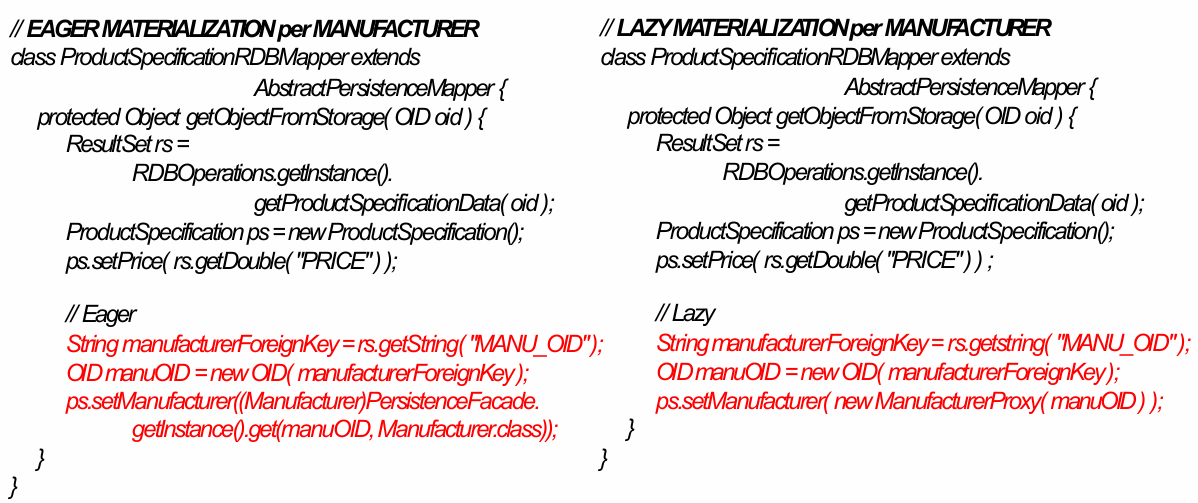
\includegraphics[scale=0.4]{Esercitazione - Design Patterns/Eager vs Lazy Materialization.png}
\end{center}

La differenza tra i due approcci sta nel caricamento in memoria del record in oggetto. Nel primo caso, avviene immediatamente
non appena i dati richiesti sono necessari, nel secondo caso il caricamento viene ritardato fino a quando l'oggetto non è
strettamente necessario.

Guardando il codice, entrambi gli approcci iniziano col prelevare la chiave\\ esterna del manifacturer, per poi creare un'ID da
associare all'oggetto (che verrà caricato in memoria) di quella chiave esterna (materializzazione: da record a oggetto).

\begin{enumerate}
    \item L'approccio \textbf{Eager} preleva direttamente l'oggetto Manufacturer \\dal database (\dots get(manuOID, Manufacturer.class))
    per poi settarlo al\\ Manufacturer oggetto.
    \item L'approccio \textbf{Lazy} agisce diversamente, crea prima un Virtual Proxy (ManufacturerProxy) dotato di identificativo
    unico (manuOID), settandolo nell'istanza di Manufacturer (ps). ManufacturerProxy rappresenta il sostituto di Manufacturer
    ma in formato più leggero e senza caricarlo in memoria direttamente.
\end{enumerate}
    
    }

\end{document}
